\documentclass[12pt]{extarticle}
\usepackage[paperwidth=18in,paperheight=7.5in]{geometry}
\usepackage{amsmath}
\usepackage{hyperref}
\usepackage{multirow}
\usepackage{pdfpages}
\usepackage[utf8]{inputenc}
\title{Kaon mixing: chiral and continuum extrapolations}
\author{R Mukherjee}
\date{\today}
\begin{document}
\maketitle
\tableofcontents
\clearpage
\begin{figure}
\centering
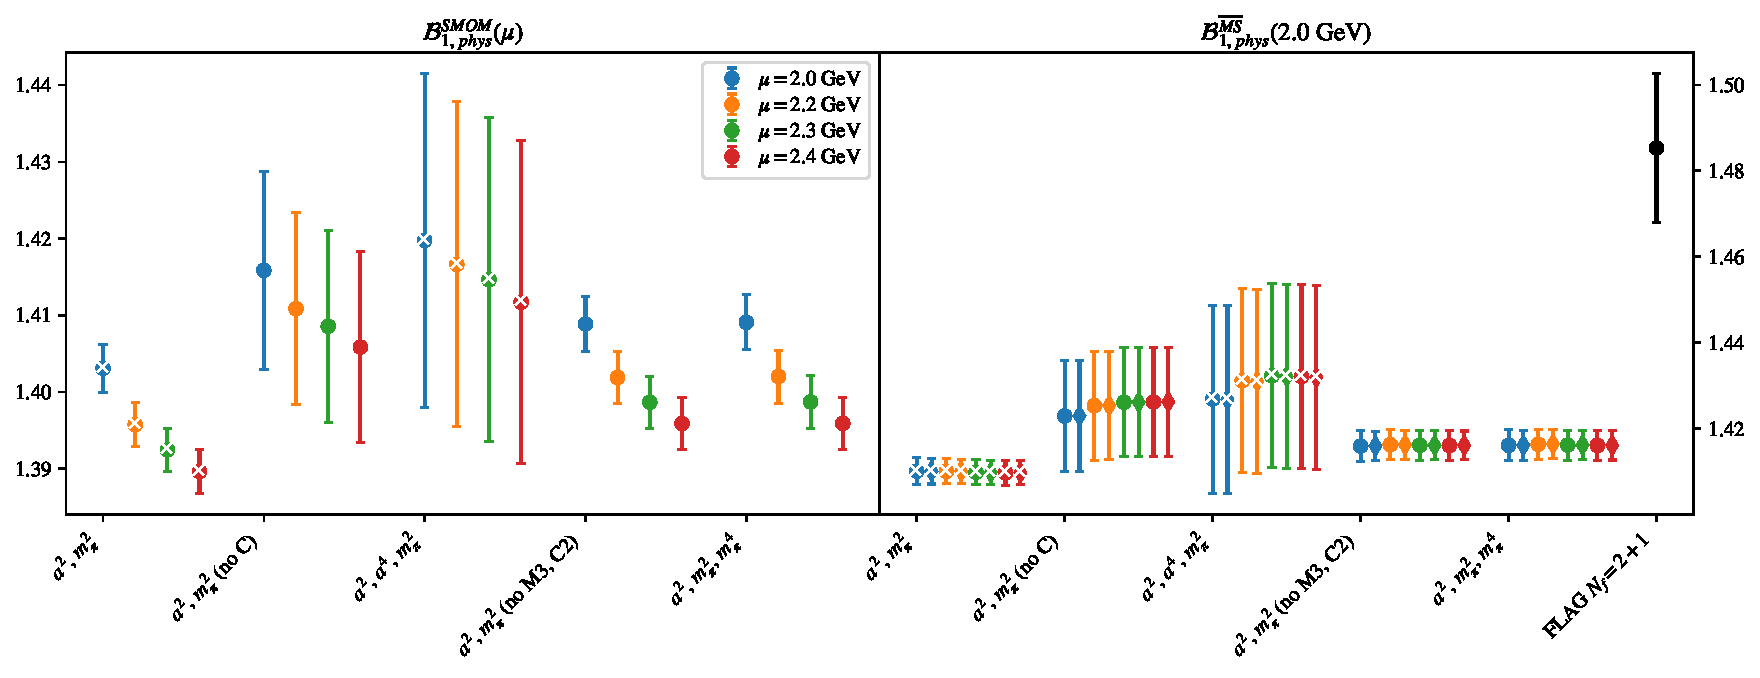
\includegraphics[page=1, width=1.1\textwidth]{VVpAA/SUSY/fit_summary_bag.pdf}
\caption{$\mathcal{B}_{1}$\\(left) $\mathcal{B}_{phys}$ in RI/SMOM scheme from fit variations (fits with $p$-value $<0.05$ marked with ``$\times$"). \\(right) $\mathcal{B}_{phys}$ in $\overline{MS}$ computed using $\mathcal{B}^{\overline{MS}} = R^{\overline{MS}\leftarrow SMOM}(2.0)\sigma_{npt}(2.0,\mu) \mathcal{B}^{SMOM}(\mu)$.}
\end{figure}
\clearpage
\begin{figure}
\centering
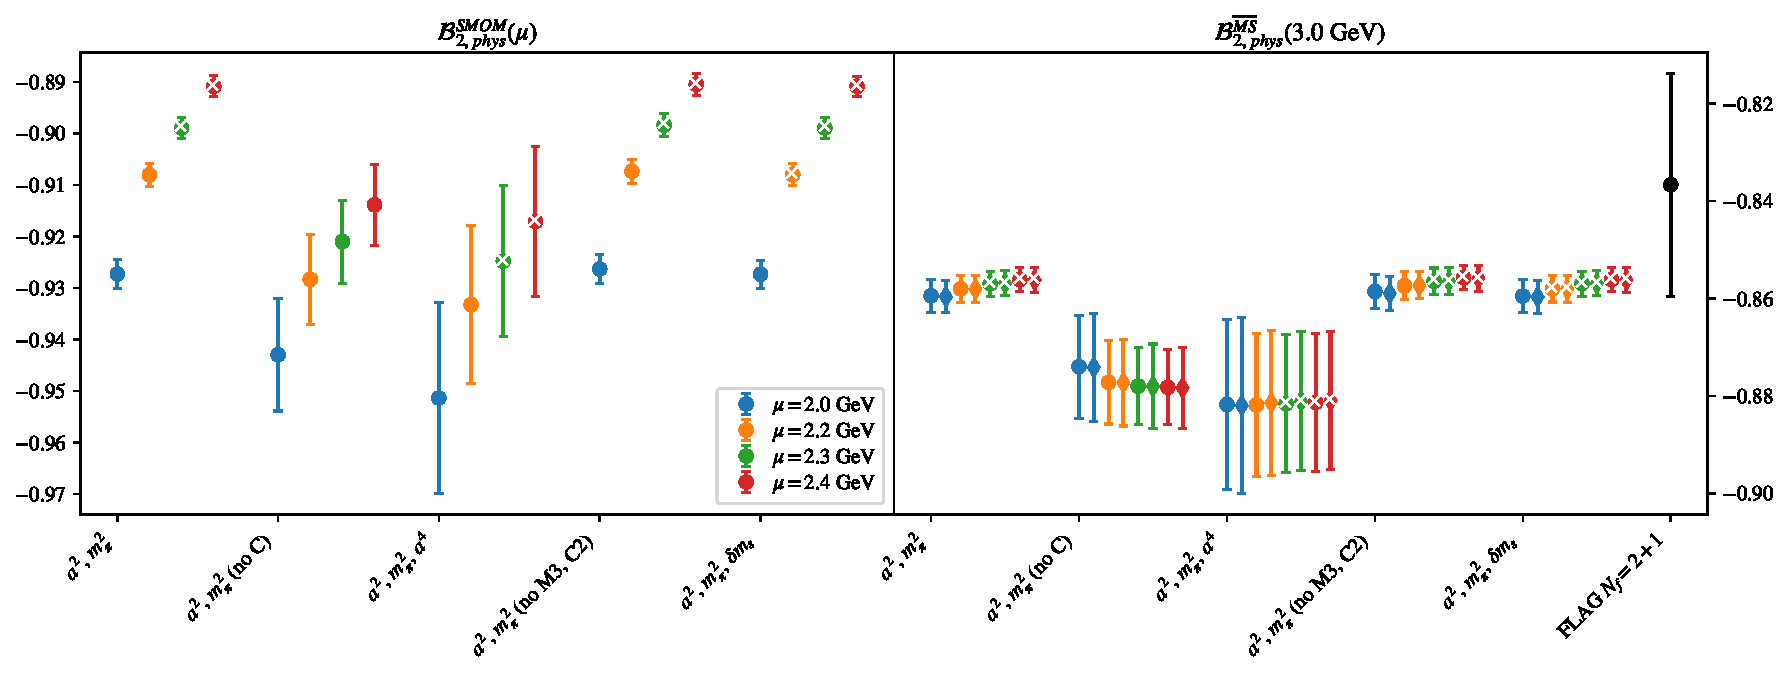
\includegraphics[page=1, width=1.1\textwidth]{VVmAA/SUSY/fit_summary_bag.pdf}
\caption{$\mathcal{B}_{2}$\\(left) $\mathcal{B}_{phys}$ in RI/SMOM scheme from fit variations (fits with $p$-value $<0.05$ marked with ``$\times$"). \\(right) $\mathcal{B}_{phys}$ in $\overline{MS}$ computed using $\mathcal{B}^{\overline{MS}} = R^{\overline{MS}\leftarrow SMOM}(3.0)\sigma_{npt}(3.0,\mu) \mathcal{B}^{SMOM}(\mu)$.}
\end{figure}
\clearpage
\begin{figure}
\centering
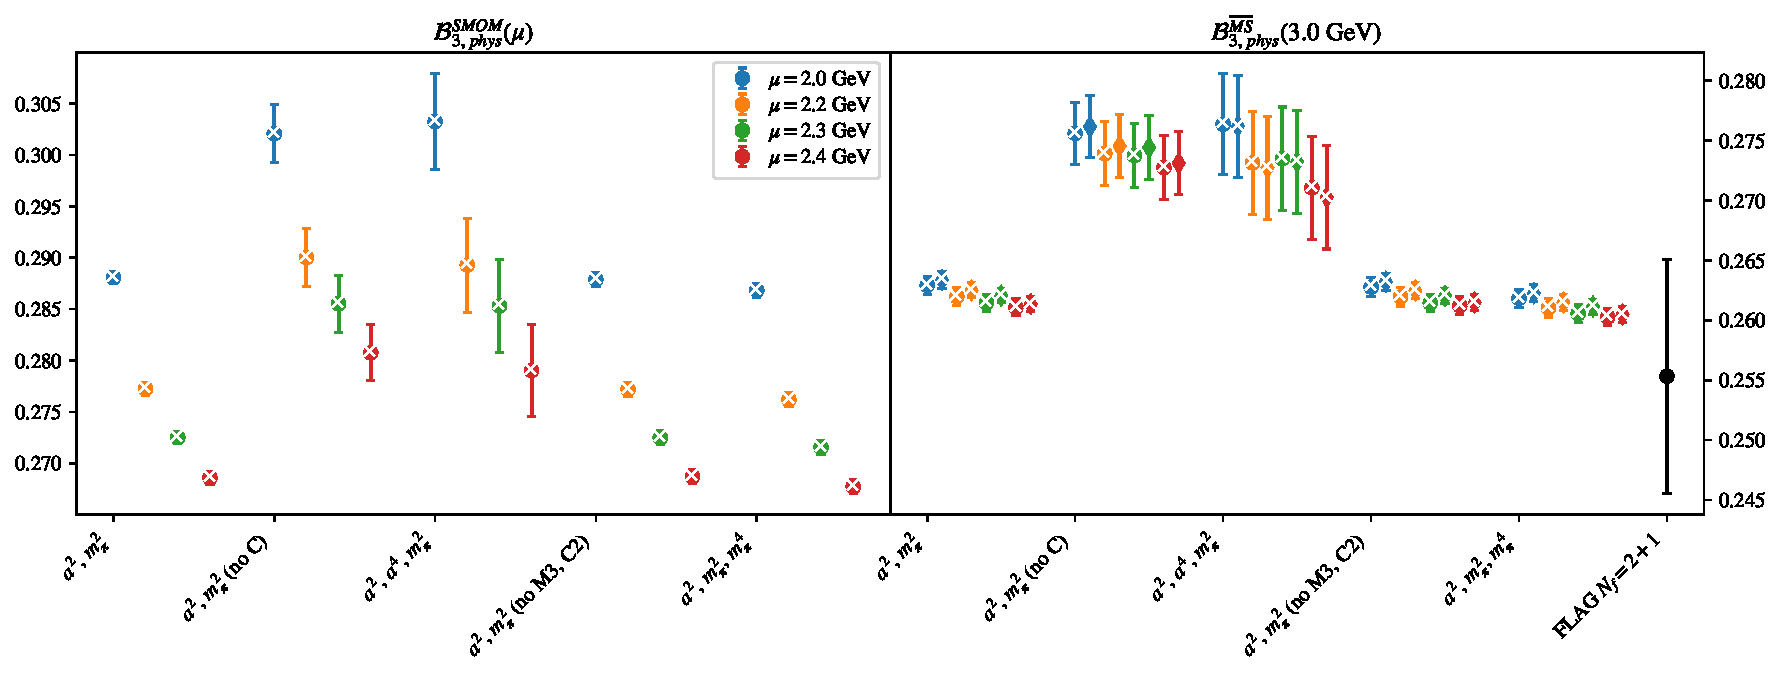
\includegraphics[page=1, width=1.1\textwidth]{SSmPP/SUSY/fit_summary_bag.pdf}
\caption{$\mathcal{B}_{3}$\\(left) $\mathcal{B}_{phys}$ in RI/SMOM scheme from fit variations (fits with $p$-value $<0.05$ marked with ``$\times$"). \\(right) $\mathcal{B}_{phys}$ in $\overline{MS}$ computed using $\mathcal{B}^{\overline{MS}} = R^{\overline{MS}\leftarrow SMOM}(3.0)\sigma_{npt}(3.0,\mu) \mathcal{B}^{SMOM}(\mu)$.}
\end{figure}
\clearpage
\begin{figure}
\centering
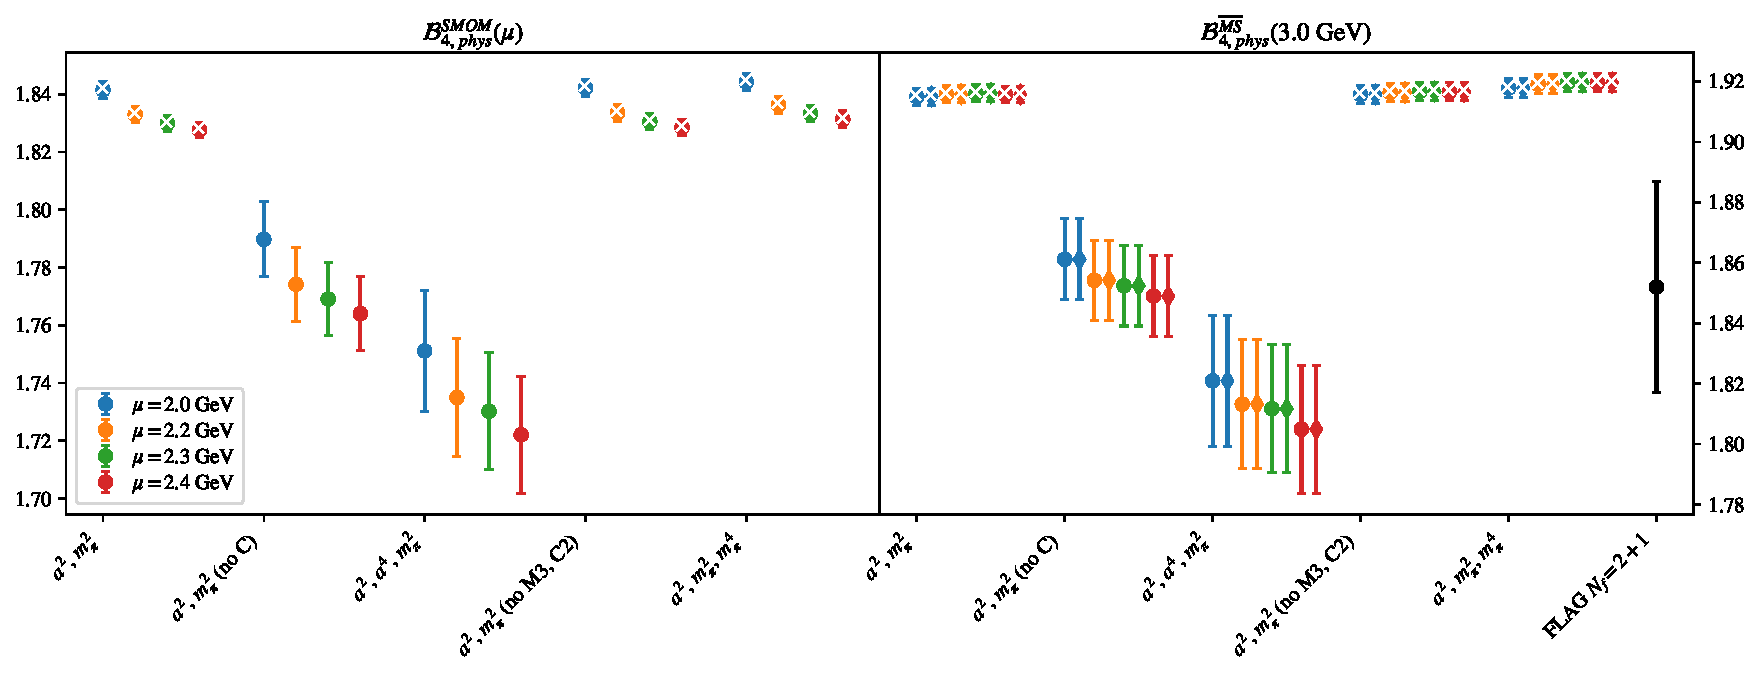
\includegraphics[page=1, width=1.1\textwidth]{SSpPP/SUSY/fit_summary_bag.pdf}
\caption{$\mathcal{B}_{4}$\\(left) $\mathcal{B}_{phys}$ in RI/SMOM scheme from fit variations (fits with $p$-value $<0.05$ marked with ``$\times$"). \\(right) $\mathcal{B}_{phys}$ in $\overline{MS}$ computed using $\mathcal{B}^{\overline{MS}} = R^{\overline{MS}\leftarrow SMOM}(3.0)\sigma_{npt}(3.0,\mu) \mathcal{B}^{SMOM}(\mu)$.}
\end{figure}
\clearpage
\begin{figure}
\centering
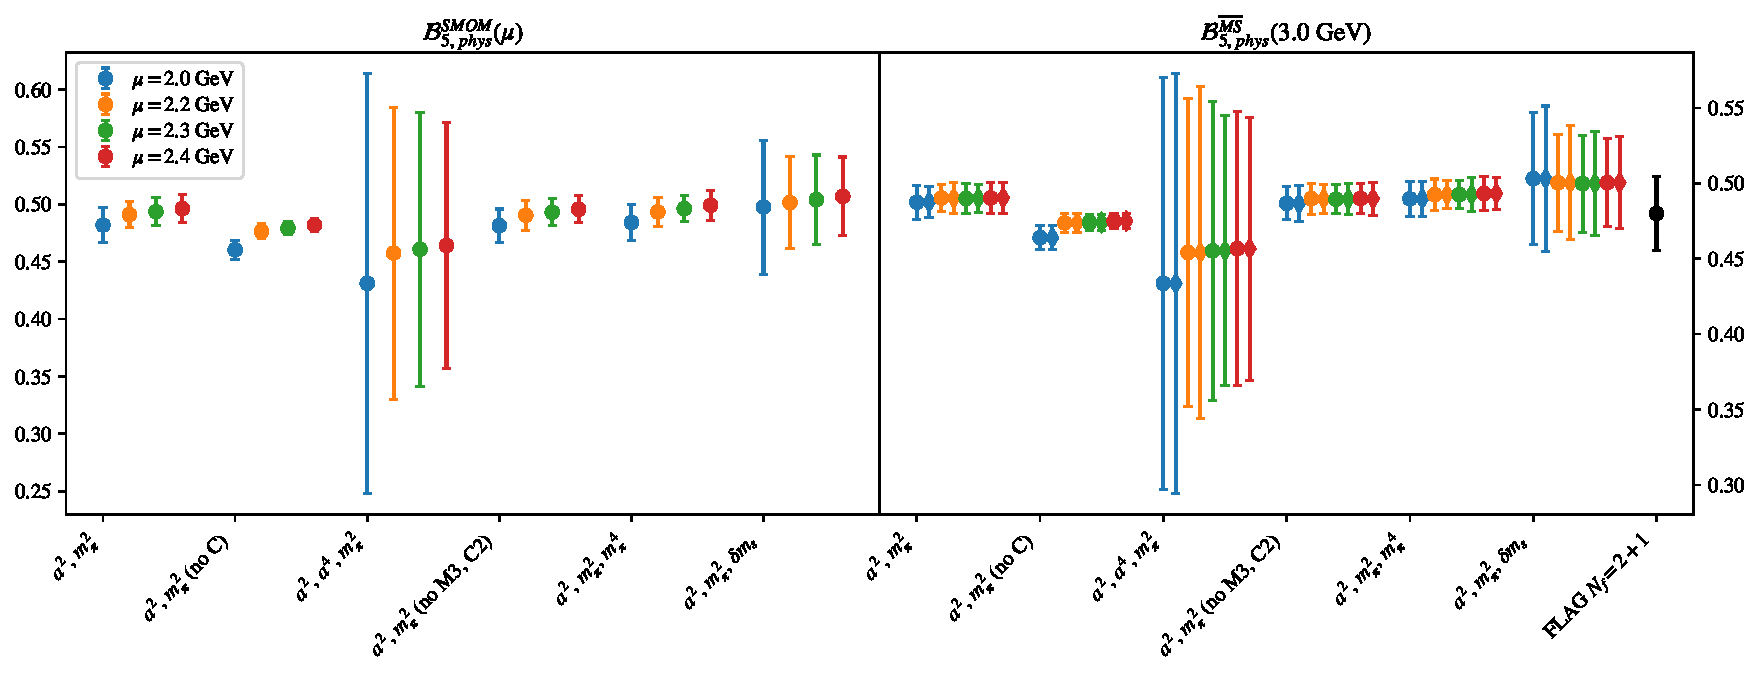
\includegraphics[page=1, width=1.1\textwidth]{TT/SUSY/fit_summary_bag.pdf}
\caption{$\mathcal{B}_{5}$\\(left) $\mathcal{B}_{phys}$ in RI/SMOM scheme from fit variations (fits with $p$-value $<0.05$ marked with ``$\times$"). \\(right) $\mathcal{B}_{phys}$ in $\overline{MS}$ computed using $\mathcal{B}^{\overline{MS}} = R^{\overline{MS}\leftarrow SMOM}(3.0)\sigma_{npt}(3.0,\mu) \mathcal{B}^{SMOM}(\mu)$.}
\end{figure}
\clearpage
\section{$\mathcal{B}_1$}
\begin{table}[h!]
\begin{center}
\begin{tabular}{|c|c|c|c|c|c|c|}
\hline
$\mu$ (GeV) & $a^2$, $m_\pi^2$& $a^2$, $m_\pi^2$ (no C)& $a^2$, $a^4$, $m_\pi^2$& $a^2$, $m_\pi^2$ (no M3, C2)& $a^2$, $m_\pi^2$, $m_\pi^4$& $a^2$, $m_\pi^2$, $\delta m_s$\\
\hline
2.0& \hyperlink{VVpAA/SUSY/a2m2_20.pdf.1}{\textbf{1.4028(61)}: 0.979 (0.429)} & \hyperlink{VVpAA/SUSY/a2m2noC_20.pdf.1}{\textbf{1.413(13)}: 0.977 (0.377)} & \hyperlink{VVpAA/SUSY/a2a4m2_20.pdf.1}{\textbf{1.424(26)}: 0.88 (0.475)} & \hyperlink{VVpAA/SUSY/a2m2mcut_20.pdf.1}{\textbf{1.4071(62)}: 0.269 (0.847)} & \hyperlink{VVpAA/SUSY/a2m2m4_20.pdf.1}{\textbf{1.4074(70)}: 0.608 (0.657)} & \hyperlink{VVpAA/SUSY/a2m2delm_20.pdf.1}{\textbf{1.3992(85)}: 0.834 (0.503)}\\
2.2& \hyperlink{VVpAA/SUSY/a2m2_22.pdf.1}{\textbf{1.3951(57)}: 1.196 (0.308)} & \hyperlink{VVpAA/SUSY/a2m2noC_22.pdf.1}{\textbf{1.410(13)}: 1.024 (0.359)} & \hyperlink{VVpAA/SUSY/a2a4m2_22.pdf.1}{\textbf{1.423(24)}: 1.068 (0.37)} & \hyperlink{VVpAA/SUSY/a2m2mcut_22.pdf.1}{\textbf{1.3998(55)}: 0.524 (0.666)} & \hyperlink{VVpAA/SUSY/a2m2m4_22.pdf.1}{\textbf{1.3997(64)}: 0.935 (0.443)} & \hyperlink{VVpAA/SUSY/a2m2delm_22.pdf.1}{\textbf{1.3909(79)}: 0.925 (0.448)}\\
2.3& \hyperlink{VVpAA/SUSY/a2m2_23.pdf.1}{\textbf{1.3922(59)}: 1.254 (0.281)} & \hyperlink{VVpAA/SUSY/a2m2noC_23.pdf.1}{\textbf{1.409(13)}: 1.046 (0.351)} & \hyperlink{VVpAA/SUSY/a2a4m2_23.pdf.1}{\textbf{1.425(23)}: 1.148 (0.332)} & \hyperlink{VVpAA/SUSY/a2m2mcut_23.pdf.1}{\textbf{1.3966(59)}: 0.666 (0.573)} & \hyperlink{VVpAA/SUSY/a2m2m4_23.pdf.1}{\textbf{1.3961(63)}: 1.117 (0.346)} & \hyperlink{VVpAA/SUSY/a2m2delm_23.pdf.1}{\textbf{1.3870(77)}: 0.941 (0.439)}\\
2.4& \hyperlink{VVpAA/SUSY/a2m2_24.pdf.1}{\textbf{1.3893(57)}: 1.32 (0.252)} & \hyperlink{VVpAA/SUSY/a2m2noC_24.pdf.1}{\textbf{1.407(13)}: 1.072 (0.342)} & \hyperlink{VVpAA/SUSY/a2a4m2_24.pdf.1}{\textbf{1.422(22)}: 1.056 (0.377)} & \hyperlink{VVpAA/SUSY/a2m2mcut_24.pdf.1}{\textbf{1.3937(53)}: 0.71 (0.546)} & \hyperlink{VVpAA/SUSY/a2m2m4_24.pdf.1}{\textbf{1.3934(72)}: 1.128 (0.341)} & \hyperlink{VVpAA/SUSY/a2m2delm_24.pdf.1}{\textbf{1.3836(73)}: 0.968 (0.424)}\\
\hline
\end{tabular}
\caption{Physical point value from chiral and continuum extrapolation at renormalisation scale $\mu$. Entries are \textbf{value(error)}: $\chi^2/\text{DOF}$ ($p$-value).}
\end{center}
\end{table}
\begin{table}[h!]
\begin{center}
\begin{tabular}{|c c|c|c|c|c|c|c|}
\hline
$\mu$ (GeV) &  & $a^2$, $m_\pi^2$& $a^2$, $m_\pi^2$ (no C)& $a^2$, $a^4$, $m_\pi^2$& $a^2$, $m_\pi^2$ (no M3, C2)& $a^2$, $m_\pi^2$, $m_\pi^4$& $a^2$, $m_\pi^2$, $\delta m_s$\\
\hline
\multirow{2}{0.5in}{2.0} & $\alpha$ & 0.105(24)& 0.060(58)& -0.04& 0.092(25)& 0.092(28)& 0.116(31)\\
 & $\beta$ & 0.00235(21)& 0.00226(27)& 0.00234(22)& 0.00186(32)& 0.001& 0.00245(24)\\
\hline
\multirow{2}{0.5in}{2.2} & $\alpha$ & 0.108(22)& 0.044(56)& -0.08& 0.094(21)& 0.095(25)& 0.120(28)\\
 & $\beta$ & 0.00236(21)& 0.00224(27)& 0.00236(21)& 0.00183(31)& 0.00062(98)& 0.00249(23)\\
\hline
\multirow{2}{0.5in}{2.3} & $\alpha$ & 0.108(24)& 0.035(56)& -0.1(15)& 0.094(23)& 0.098(24)& 0.122(27)\\
 & $\beta$ & 0.00234(21)& 0.00224(27)& 0.00239(20)& 0.00183(32)& 0.00066(99)& 0.00251(22)\\
\hline
\multirow{2}{0.5in}{2.4} & $\alpha$ & 0.109(22)& 0.032(55)& -0.1(14)& 0.096(21)& 0.098(27)& 0.124(26)\\
 & $\beta$ & 0.00235(20)& 0.00223(27)& 0.00236(21)& 0.00180(31)& 0.001& 0.00253(21)\\
\hline
\end{tabular}
\caption{Fit values of coefficients in $Q = Q_{phys} + \mathbf{\alpha} a^2 + \mathbf{\beta}\left(\frac{m_\pi^2}{f_\pi^2}-\frac{m_{\pi,PDG}^2}{f_\pi^2}\right) + \ldots$.}
\end{center}
\end{table}
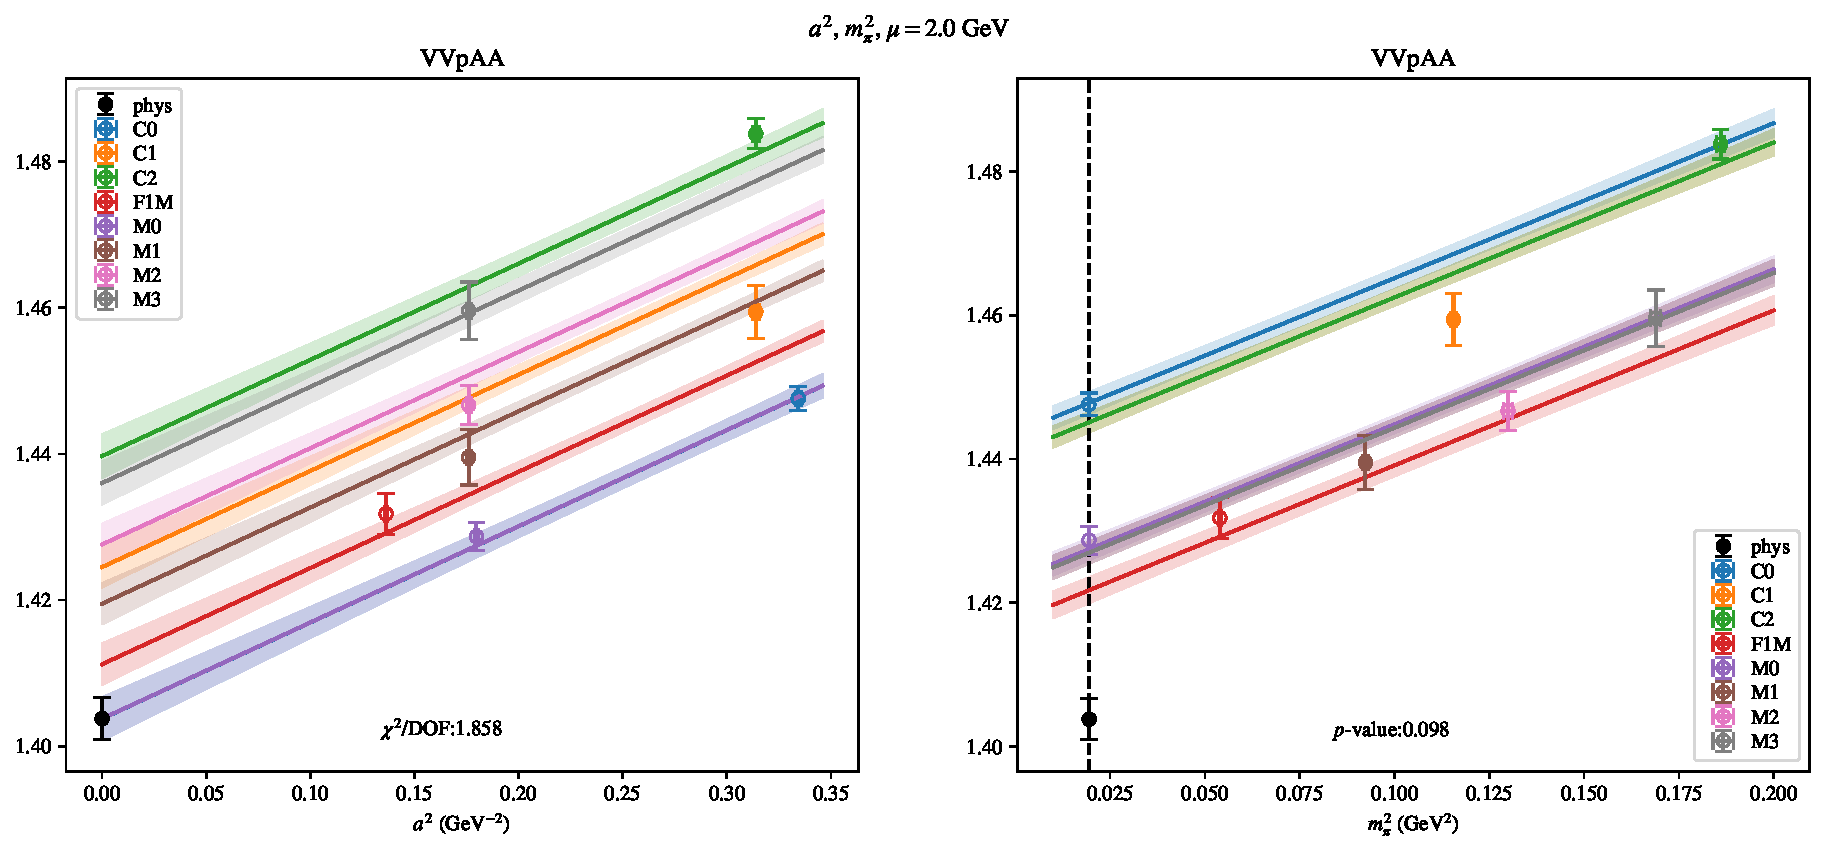
\includepdf[link, pages=-]{VVpAA/SUSY/a2m2_20.pdf}
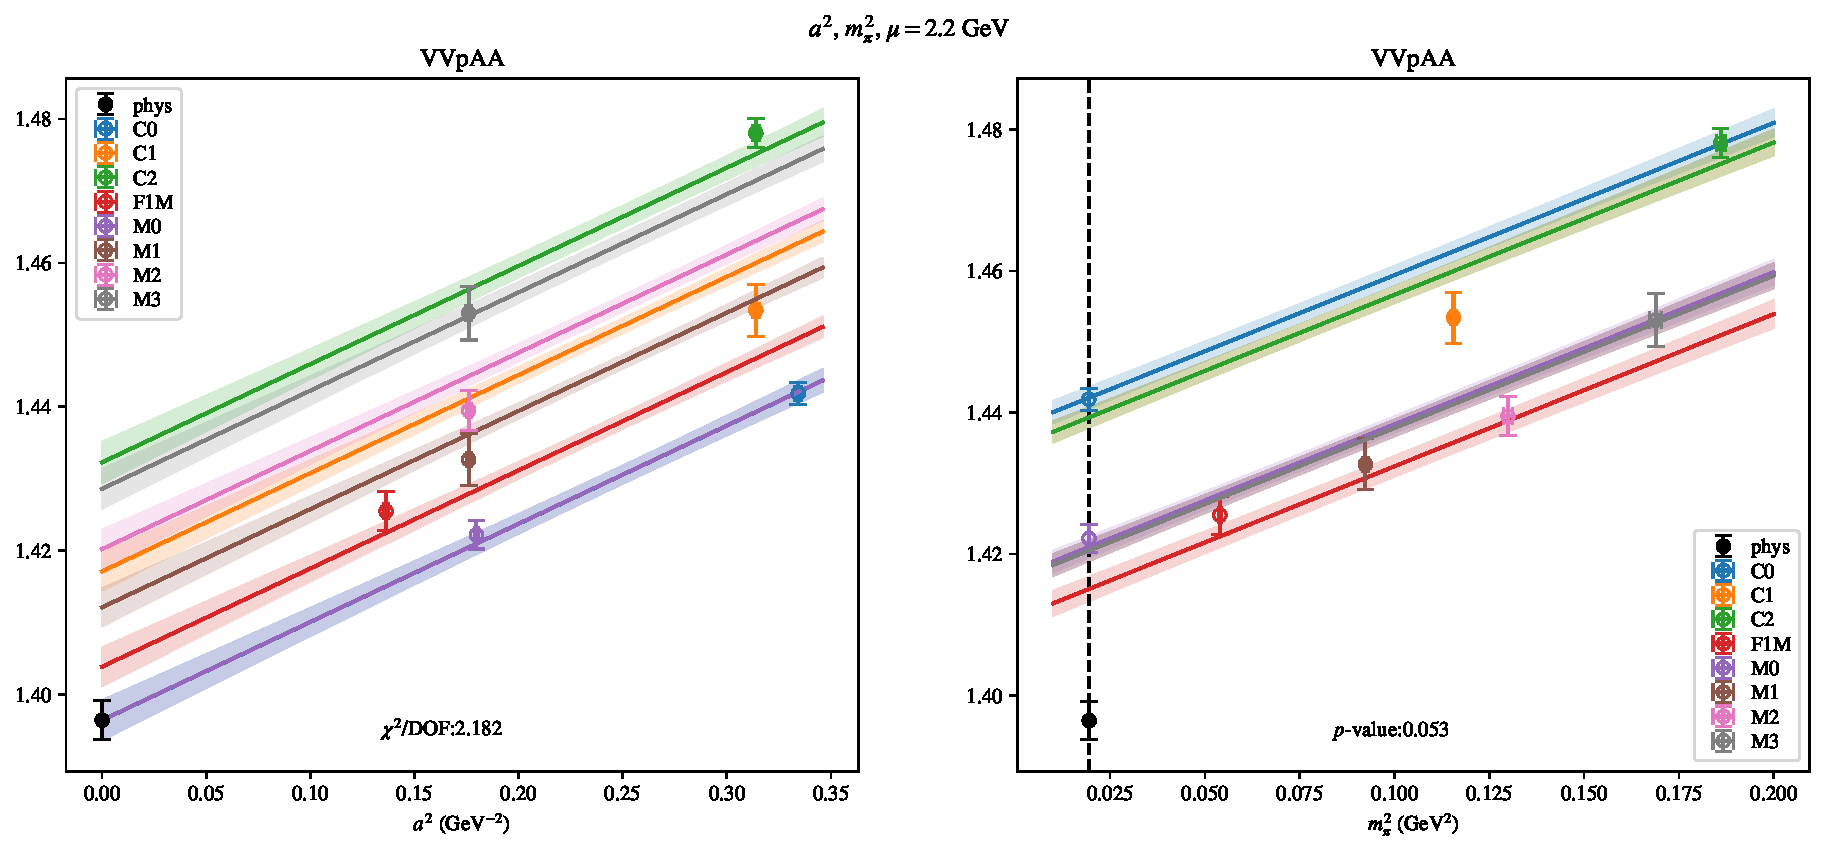
\includepdf[link, pages=-]{VVpAA/SUSY/a2m2_22.pdf}
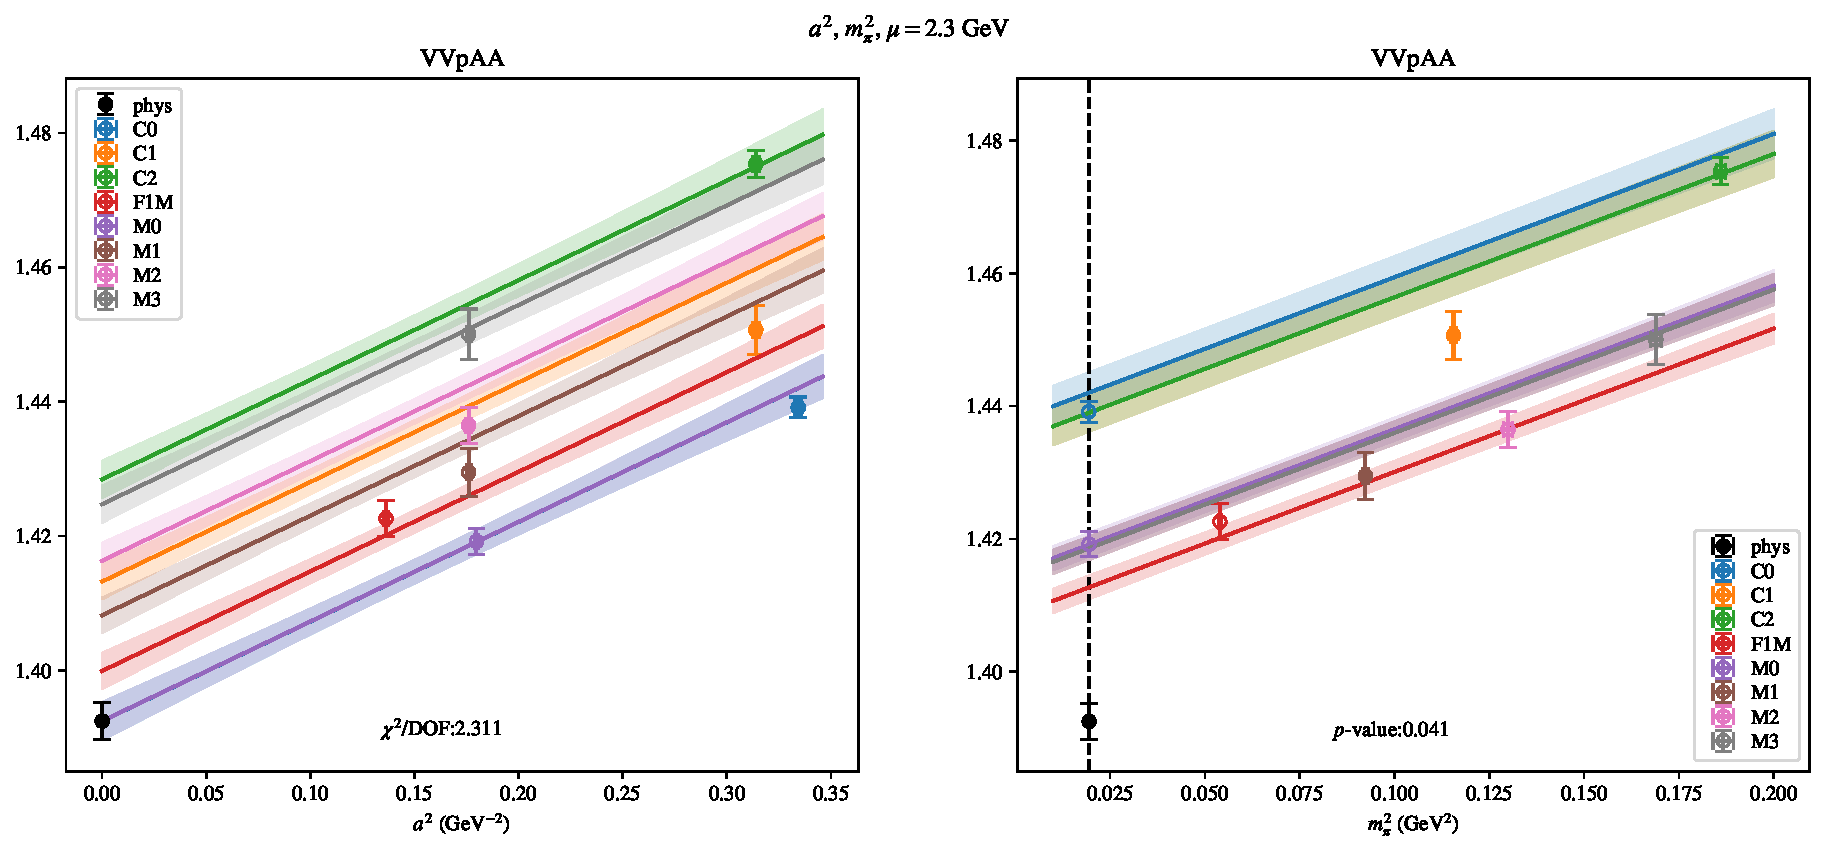
\includepdf[link, pages=-]{VVpAA/SUSY/a2m2_23.pdf}
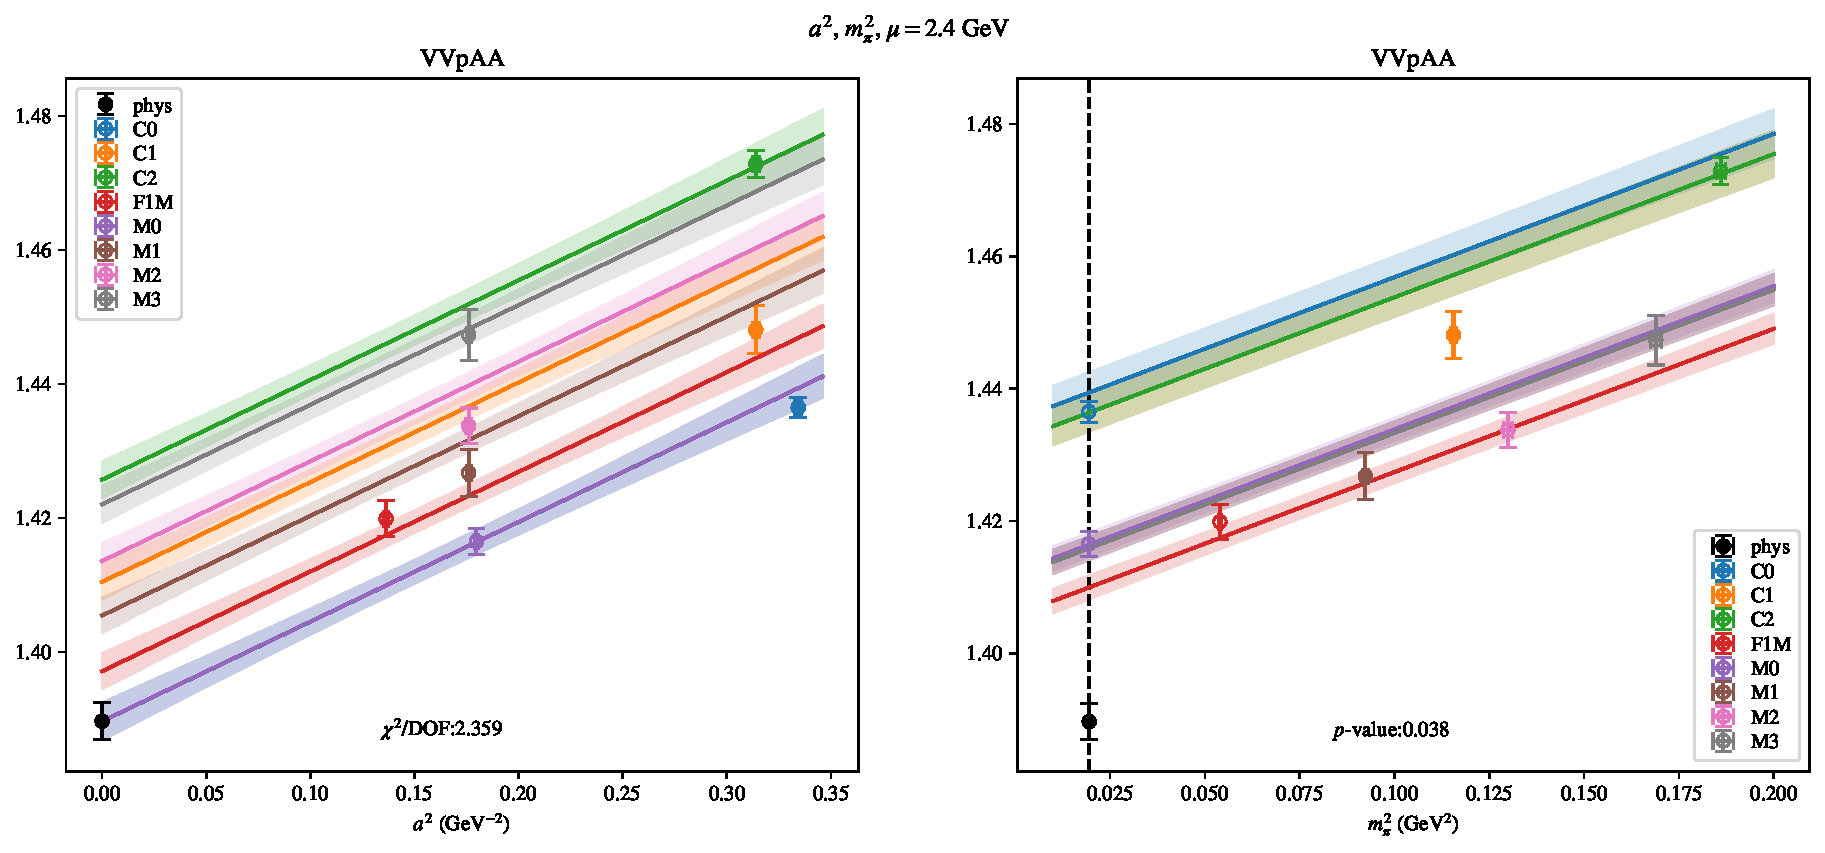
\includepdf[link, pages=-]{VVpAA/SUSY/a2m2_24.pdf}
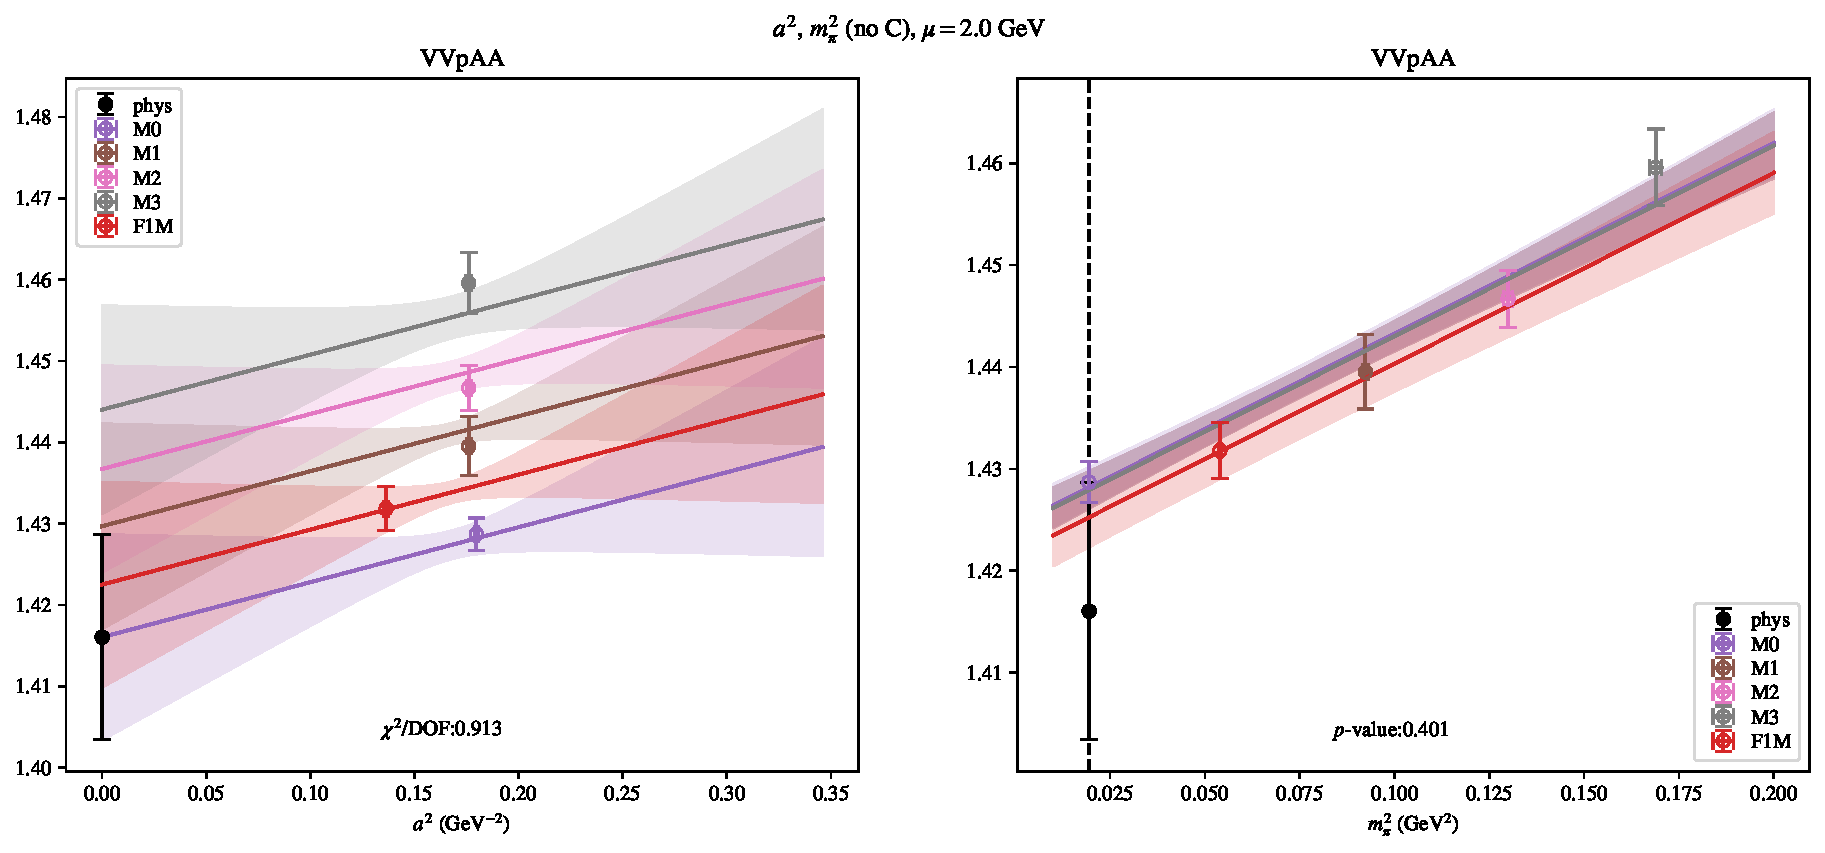
\includepdf[link, pages=-]{VVpAA/SUSY/a2m2noC_20.pdf}
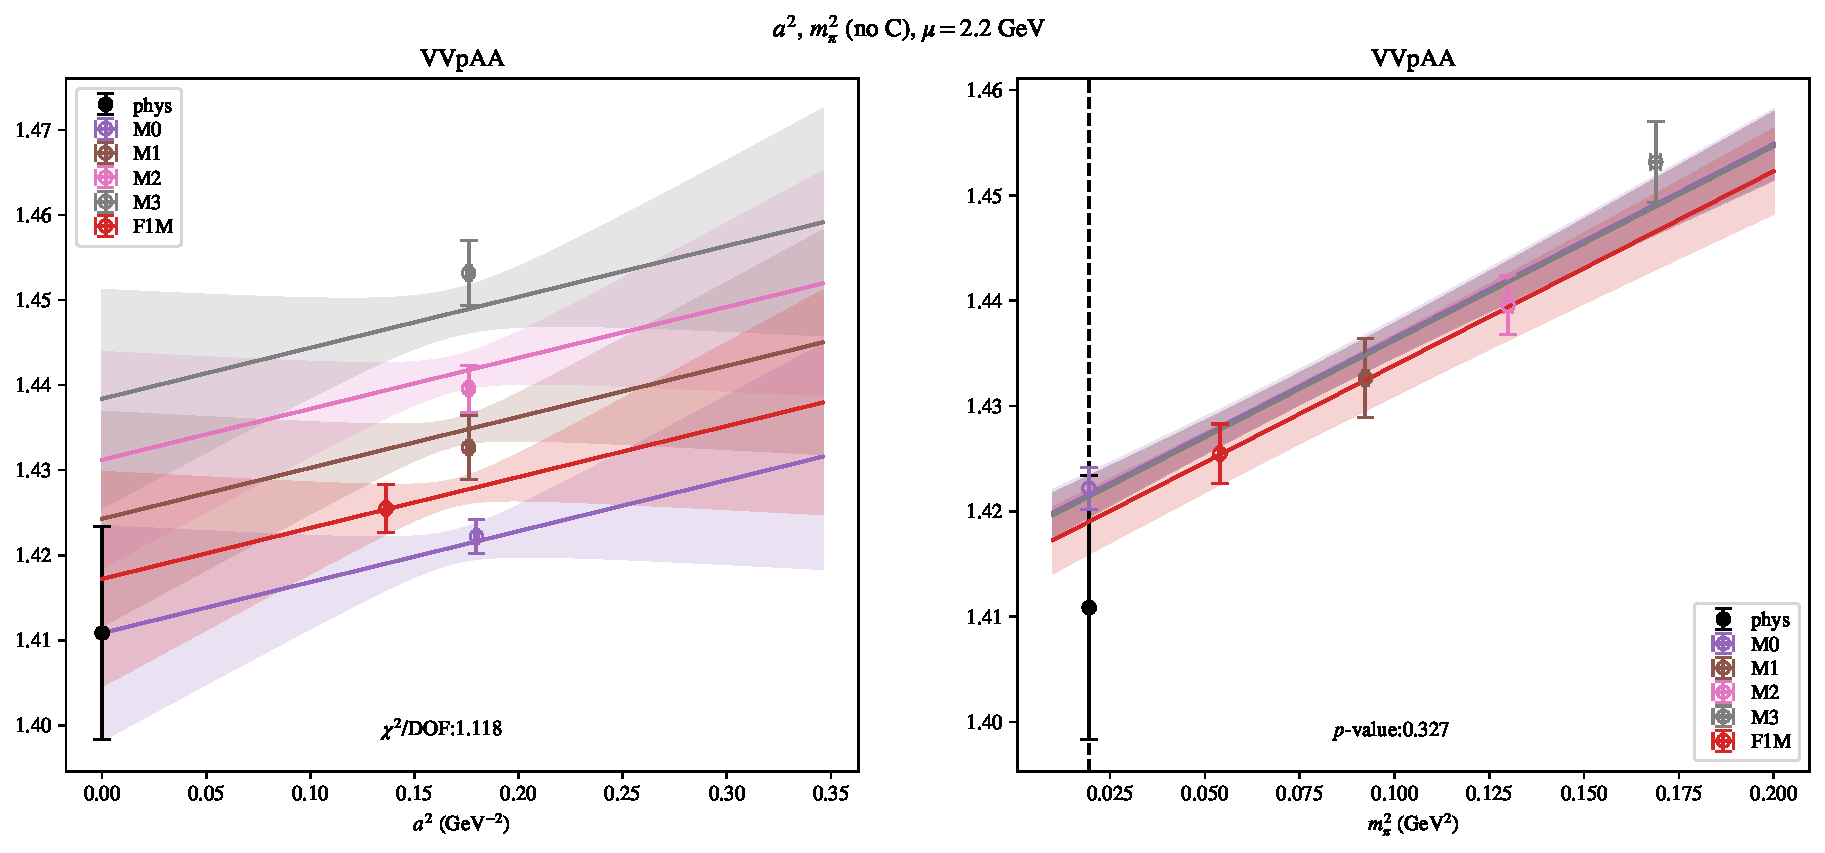
\includepdf[link, pages=-]{VVpAA/SUSY/a2m2noC_22.pdf}
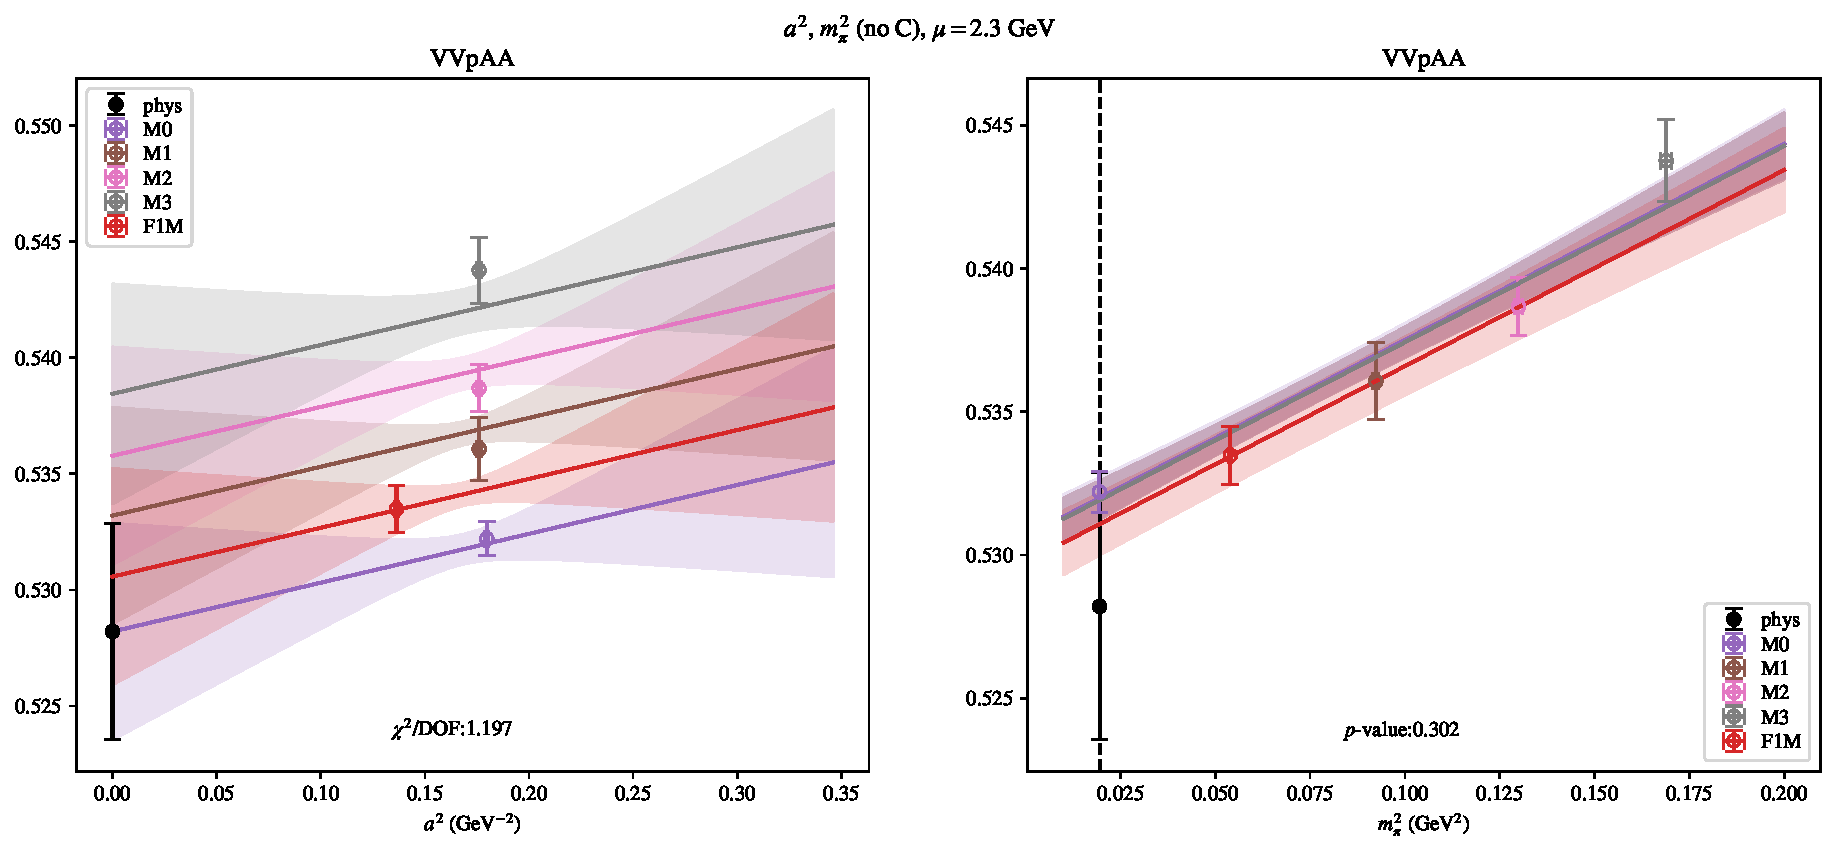
\includepdf[link, pages=-]{VVpAA/SUSY/a2m2noC_23.pdf}
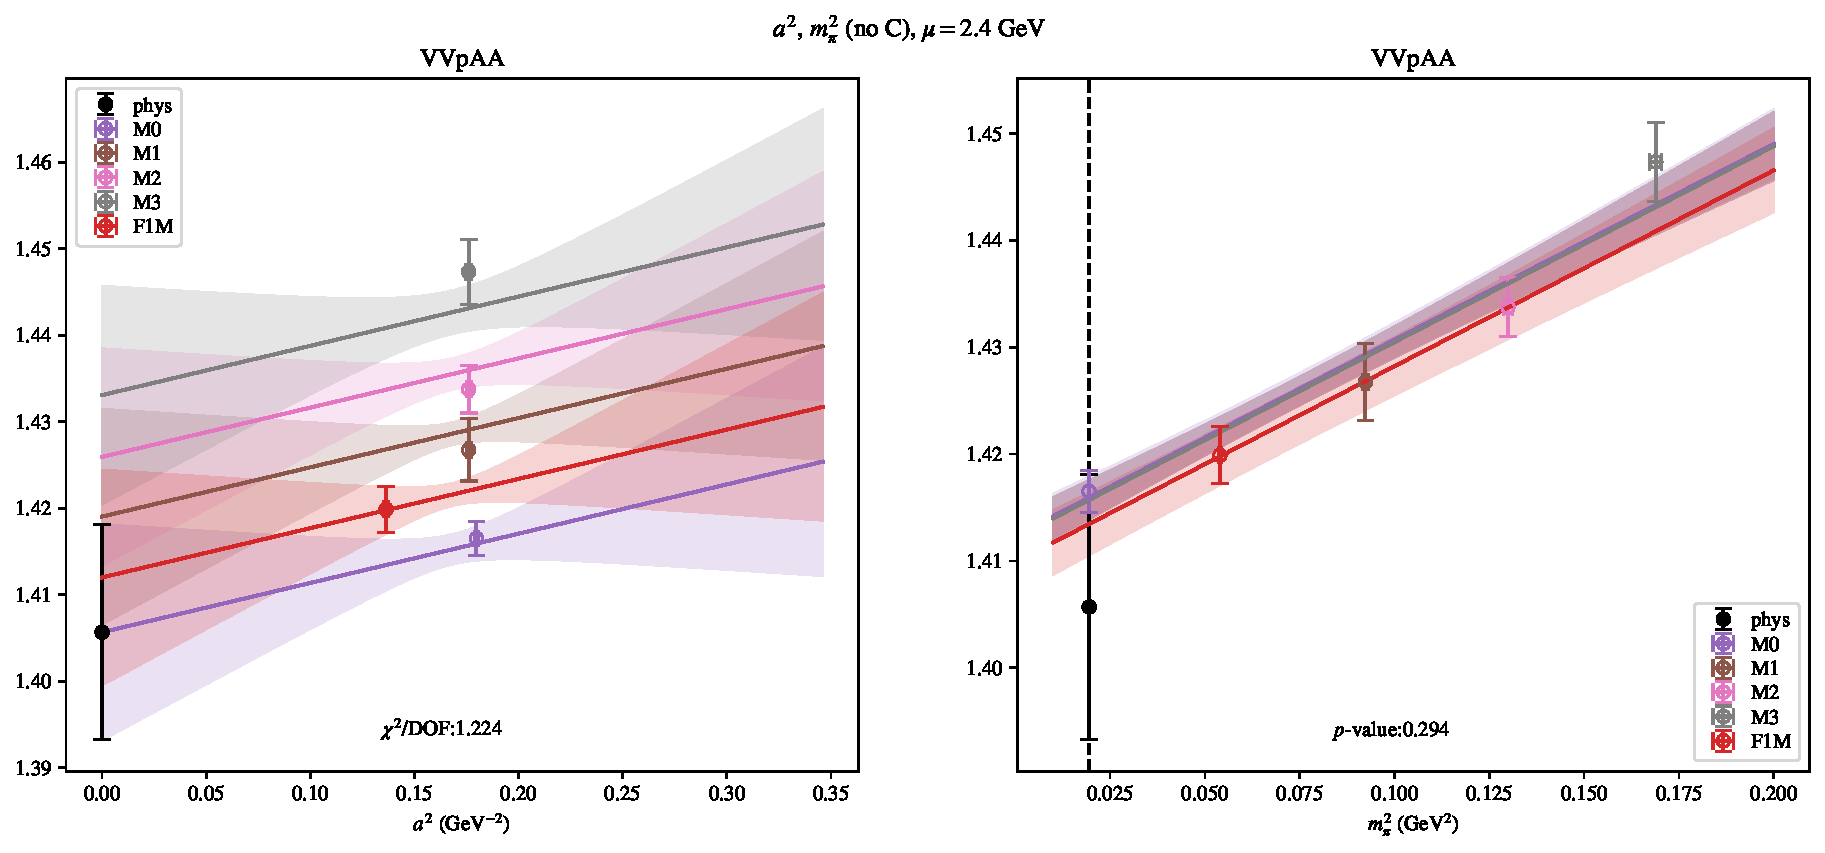
\includepdf[link, pages=-]{VVpAA/SUSY/a2m2noC_24.pdf}
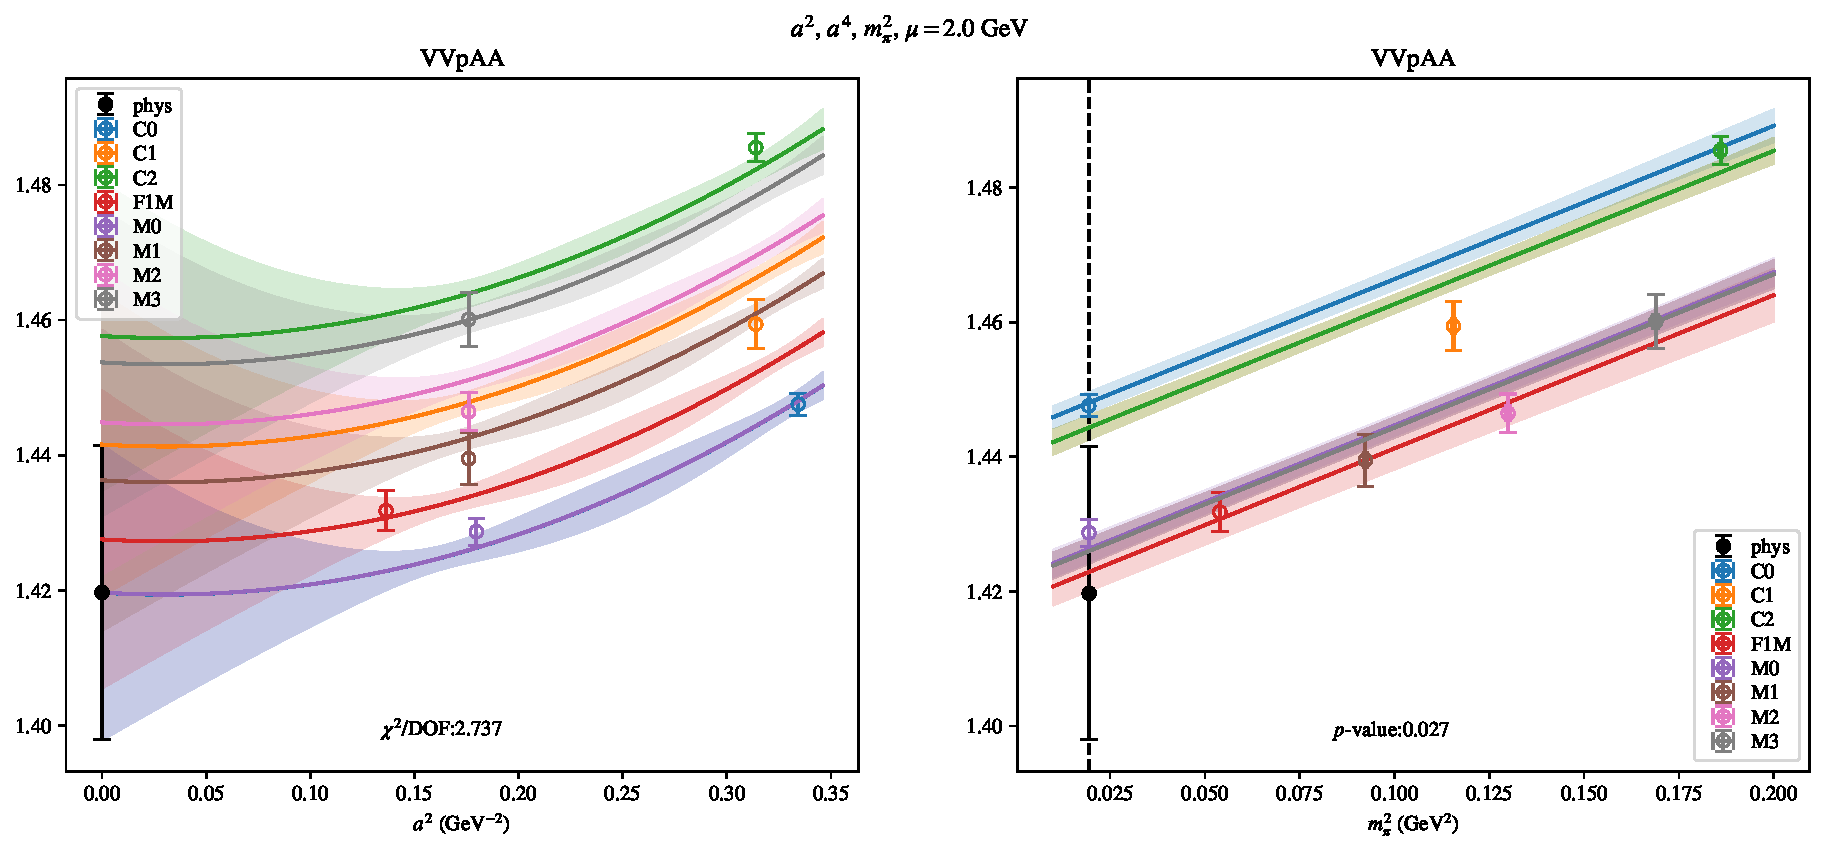
\includepdf[link, pages=-]{VVpAA/SUSY/a2a4m2_20.pdf}
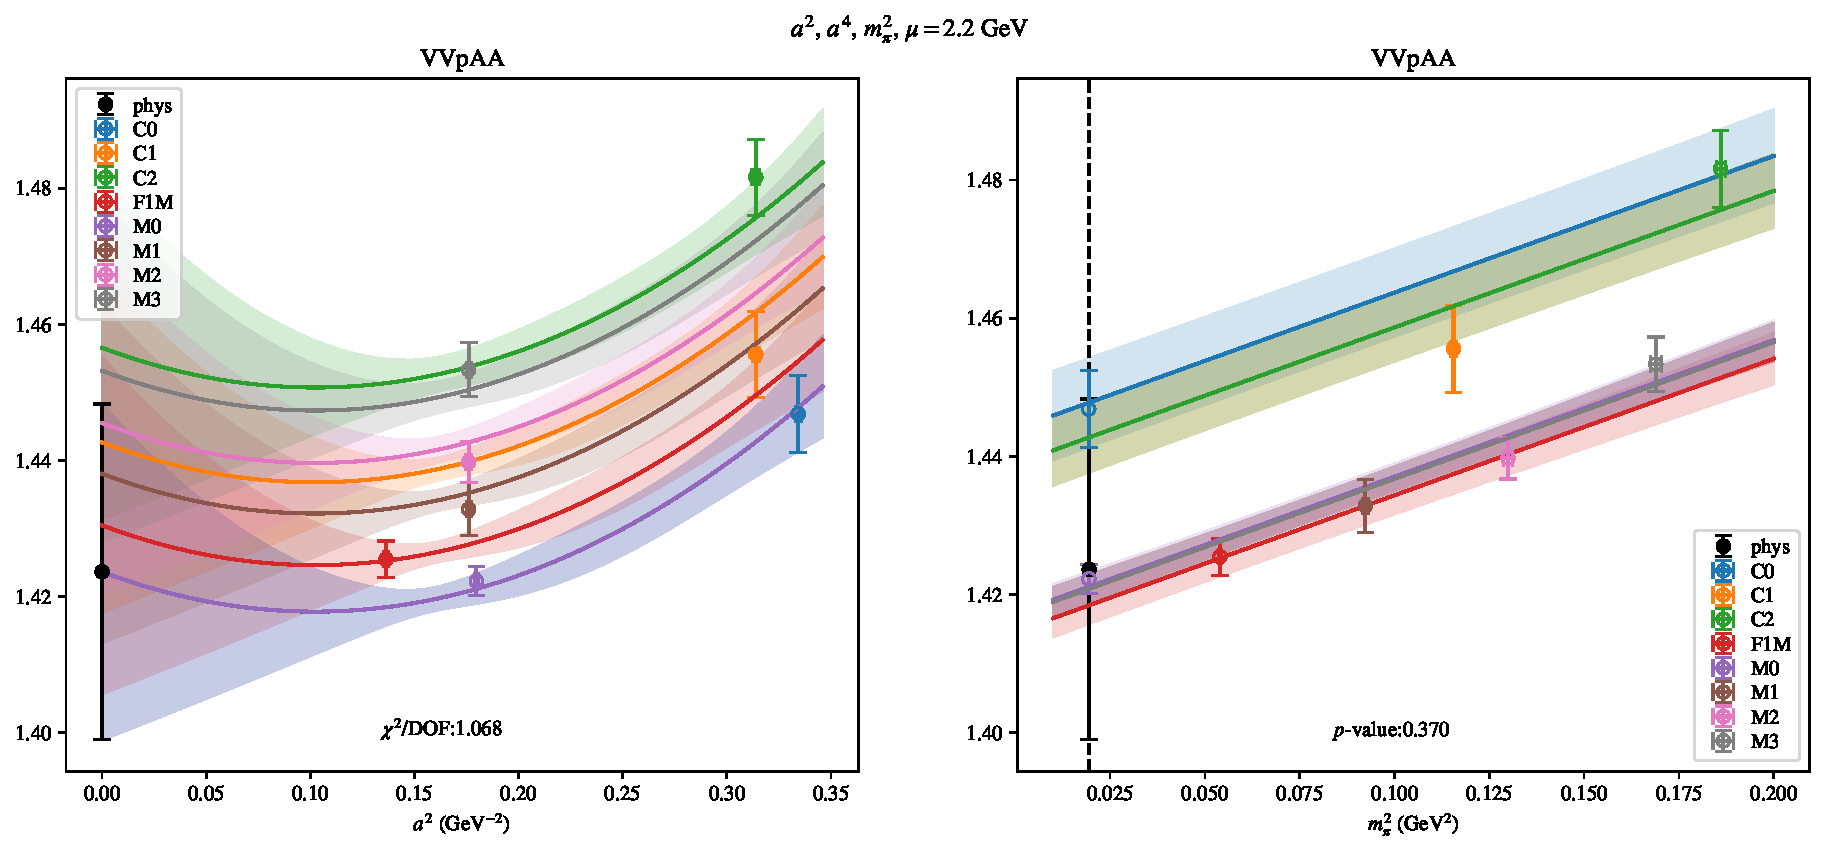
\includepdf[link, pages=-]{VVpAA/SUSY/a2a4m2_22.pdf}
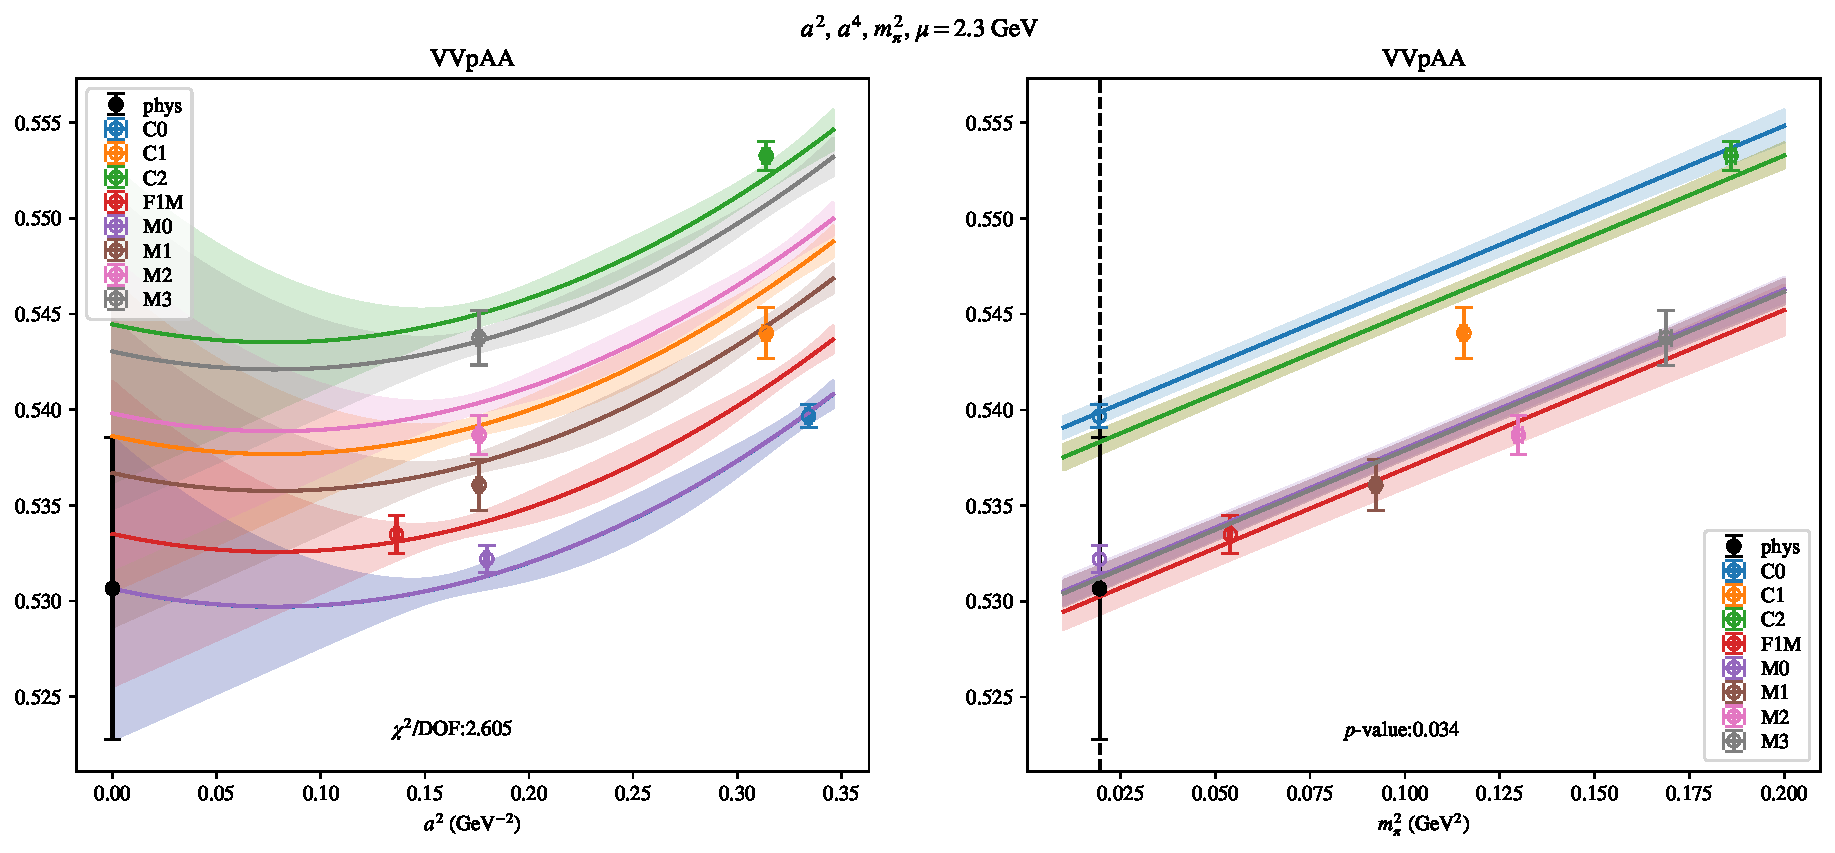
\includepdf[link, pages=-]{VVpAA/SUSY/a2a4m2_23.pdf}
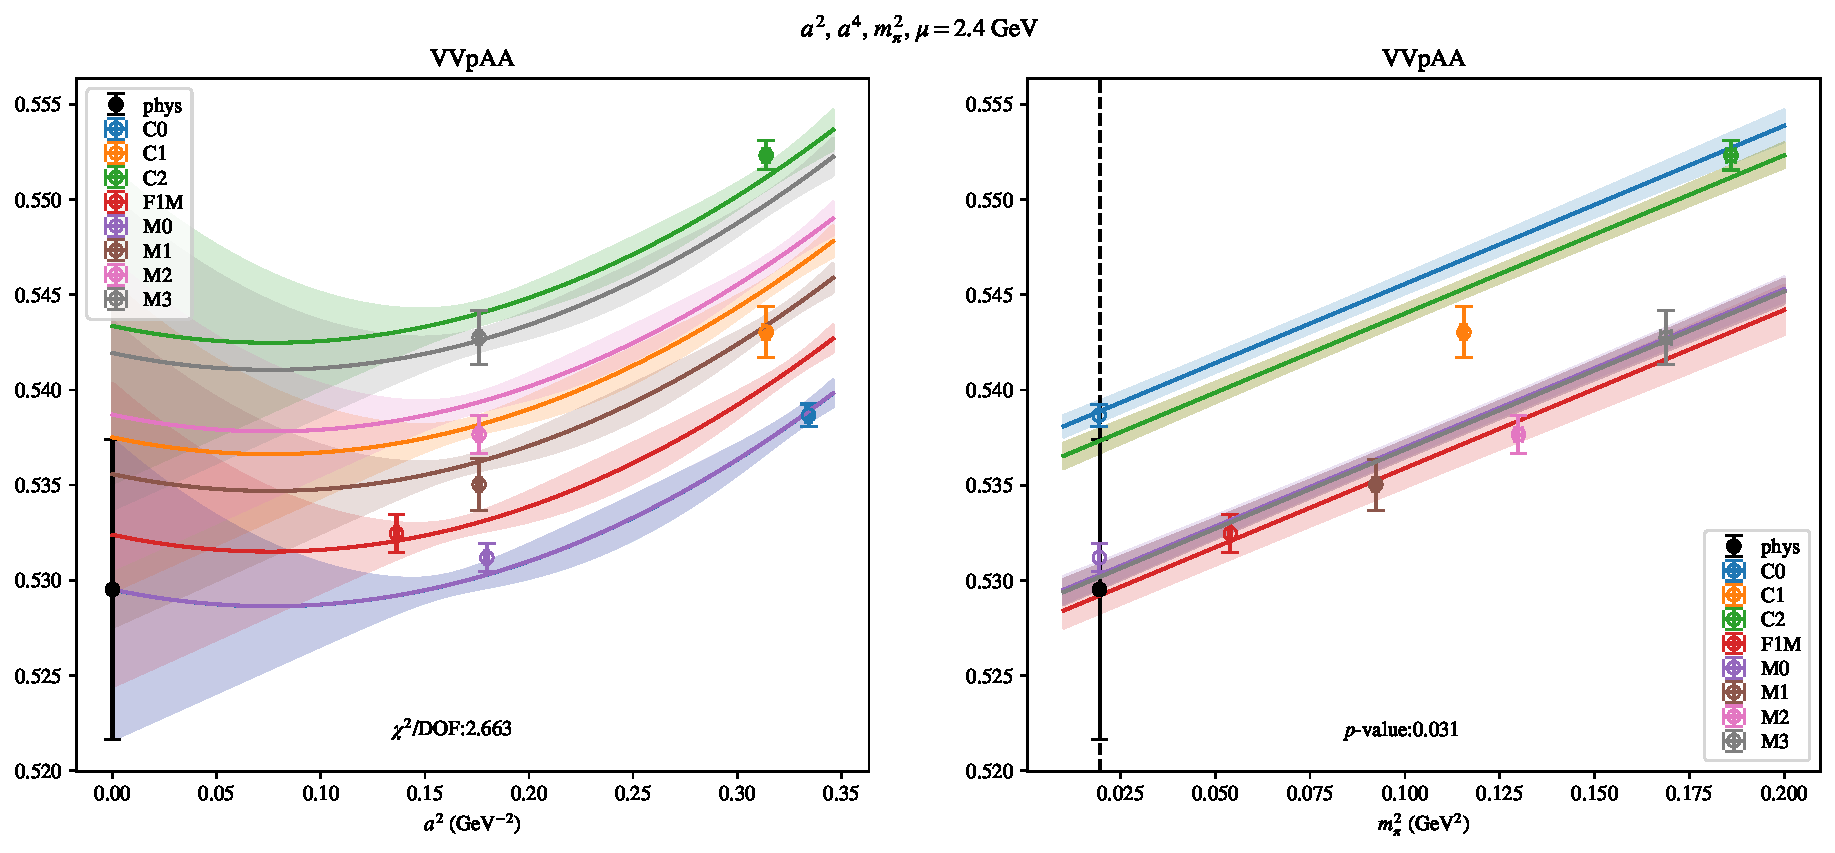
\includepdf[link, pages=-]{VVpAA/SUSY/a2a4m2_24.pdf}
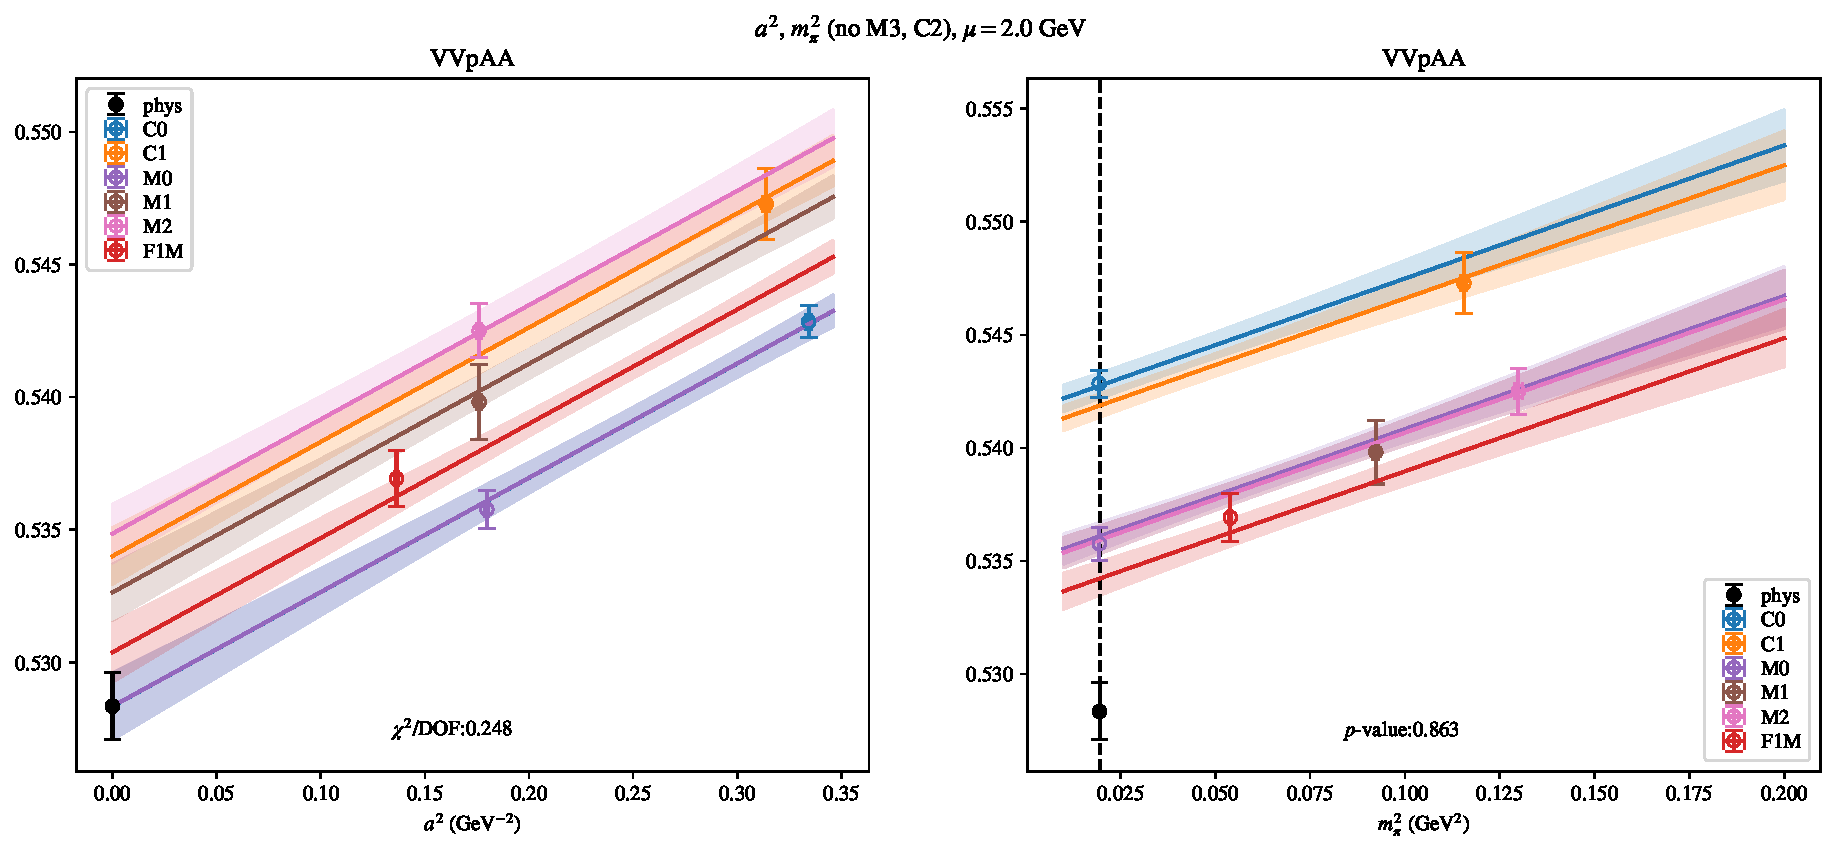
\includepdf[link, pages=-]{VVpAA/SUSY/a2m2mcut_20.pdf}
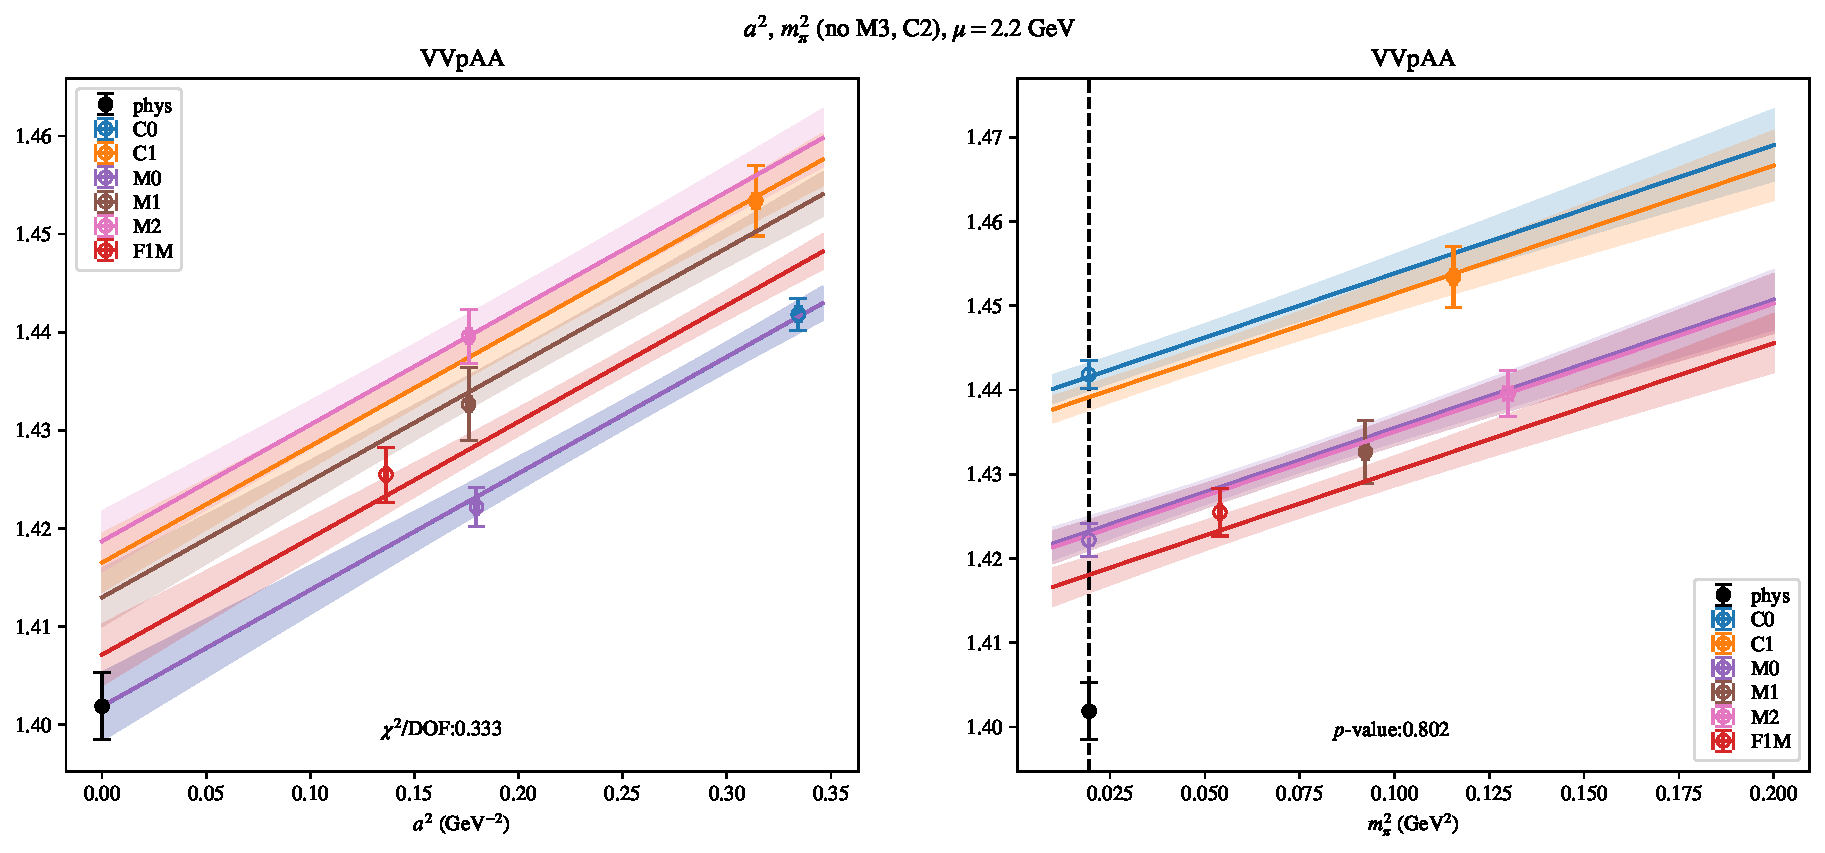
\includepdf[link, pages=-]{VVpAA/SUSY/a2m2mcut_22.pdf}
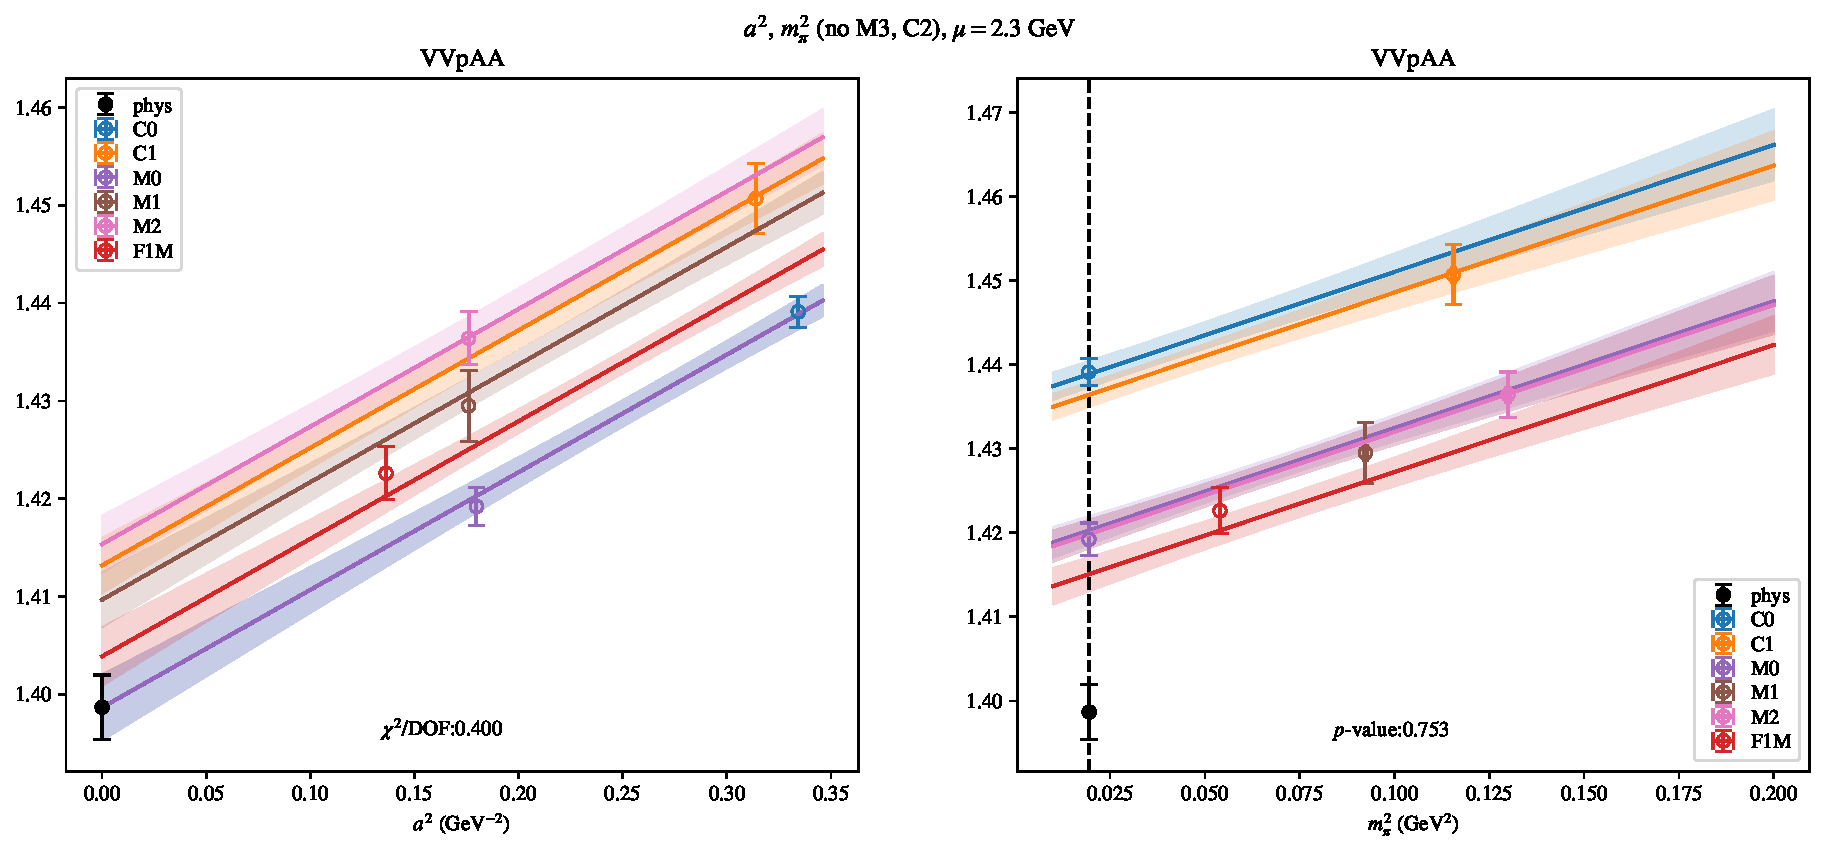
\includepdf[link, pages=-]{VVpAA/SUSY/a2m2mcut_23.pdf}
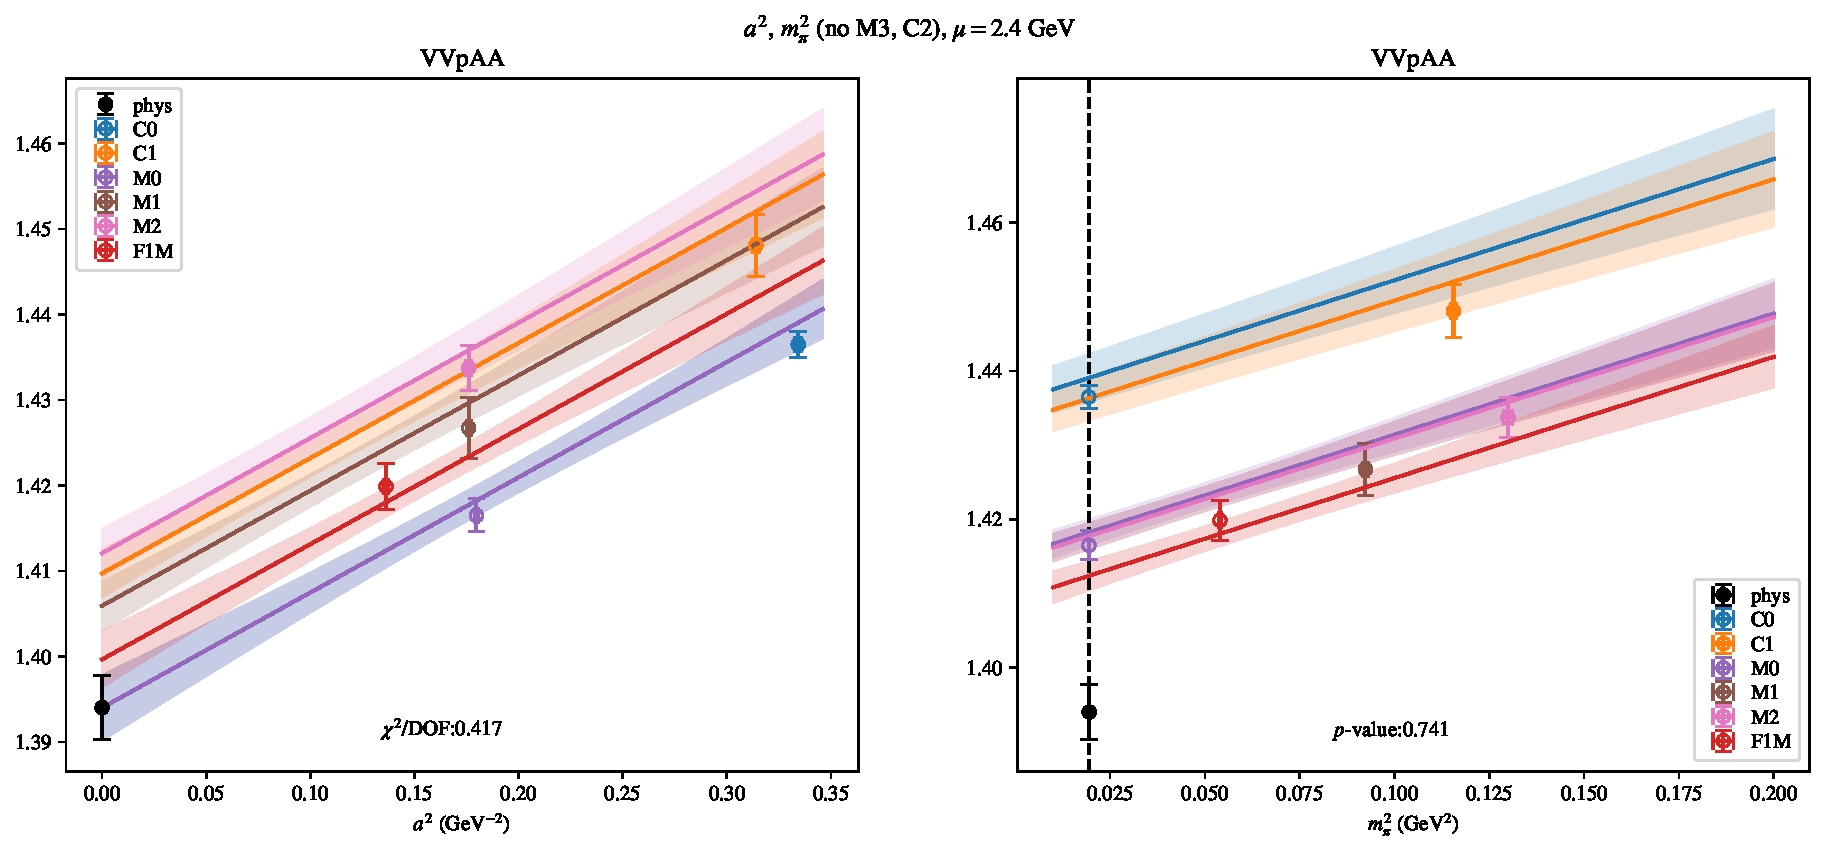
\includepdf[link, pages=-]{VVpAA/SUSY/a2m2mcut_24.pdf}
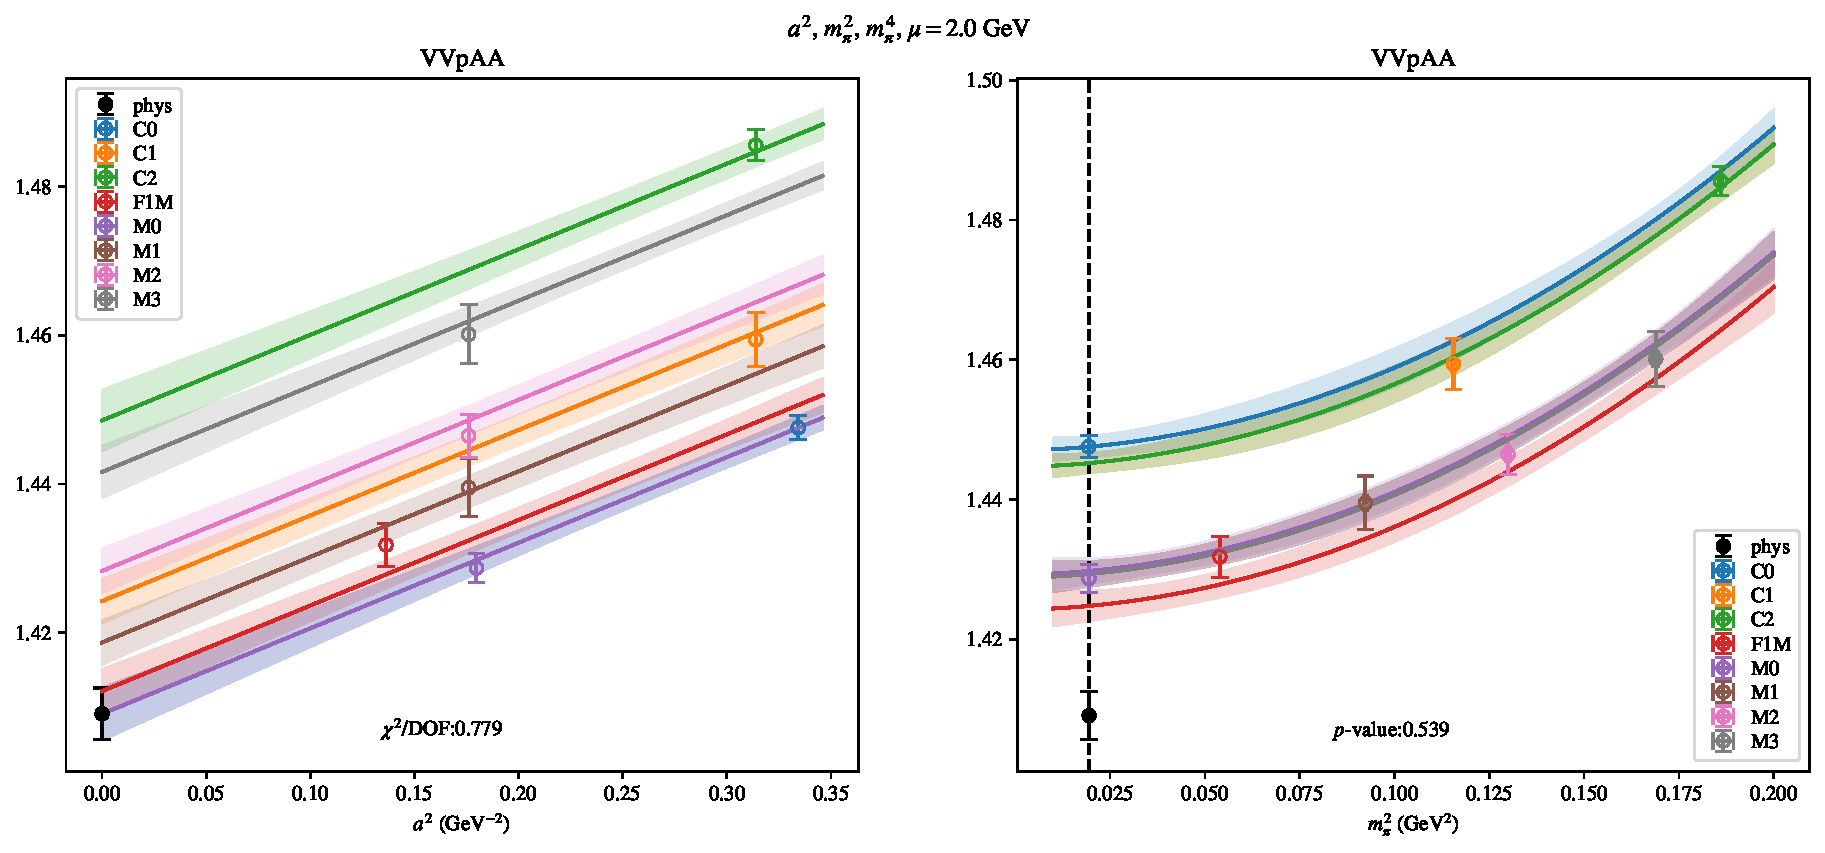
\includepdf[link, pages=-]{VVpAA/SUSY/a2m2m4_20.pdf}
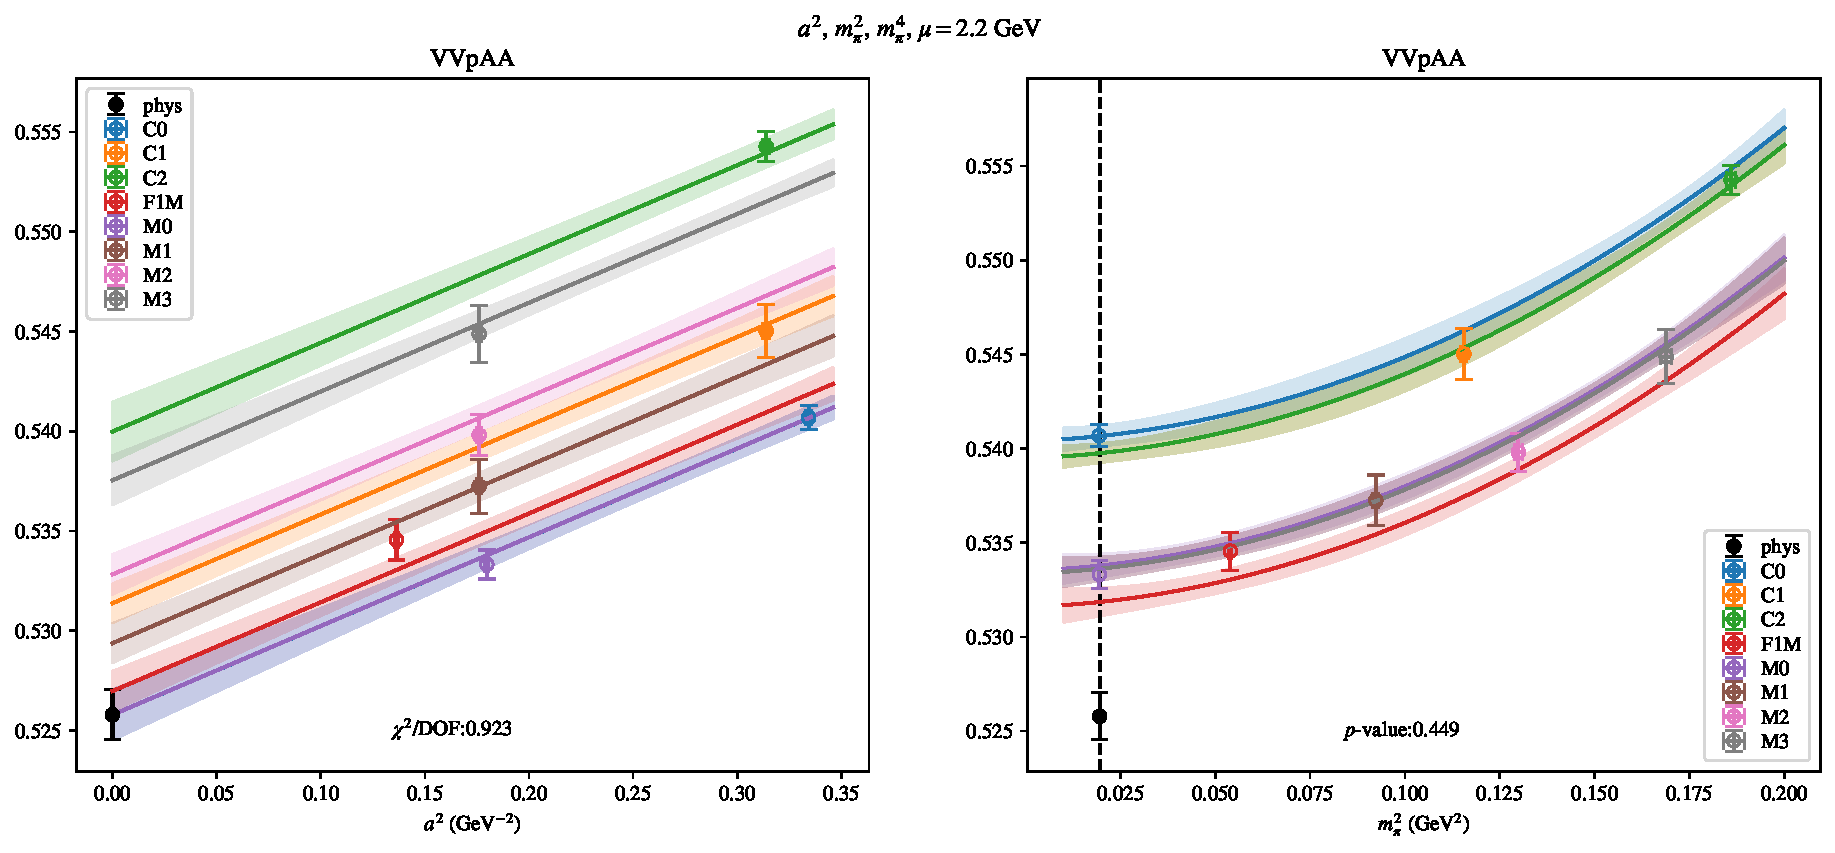
\includepdf[link, pages=-]{VVpAA/SUSY/a2m2m4_22.pdf}
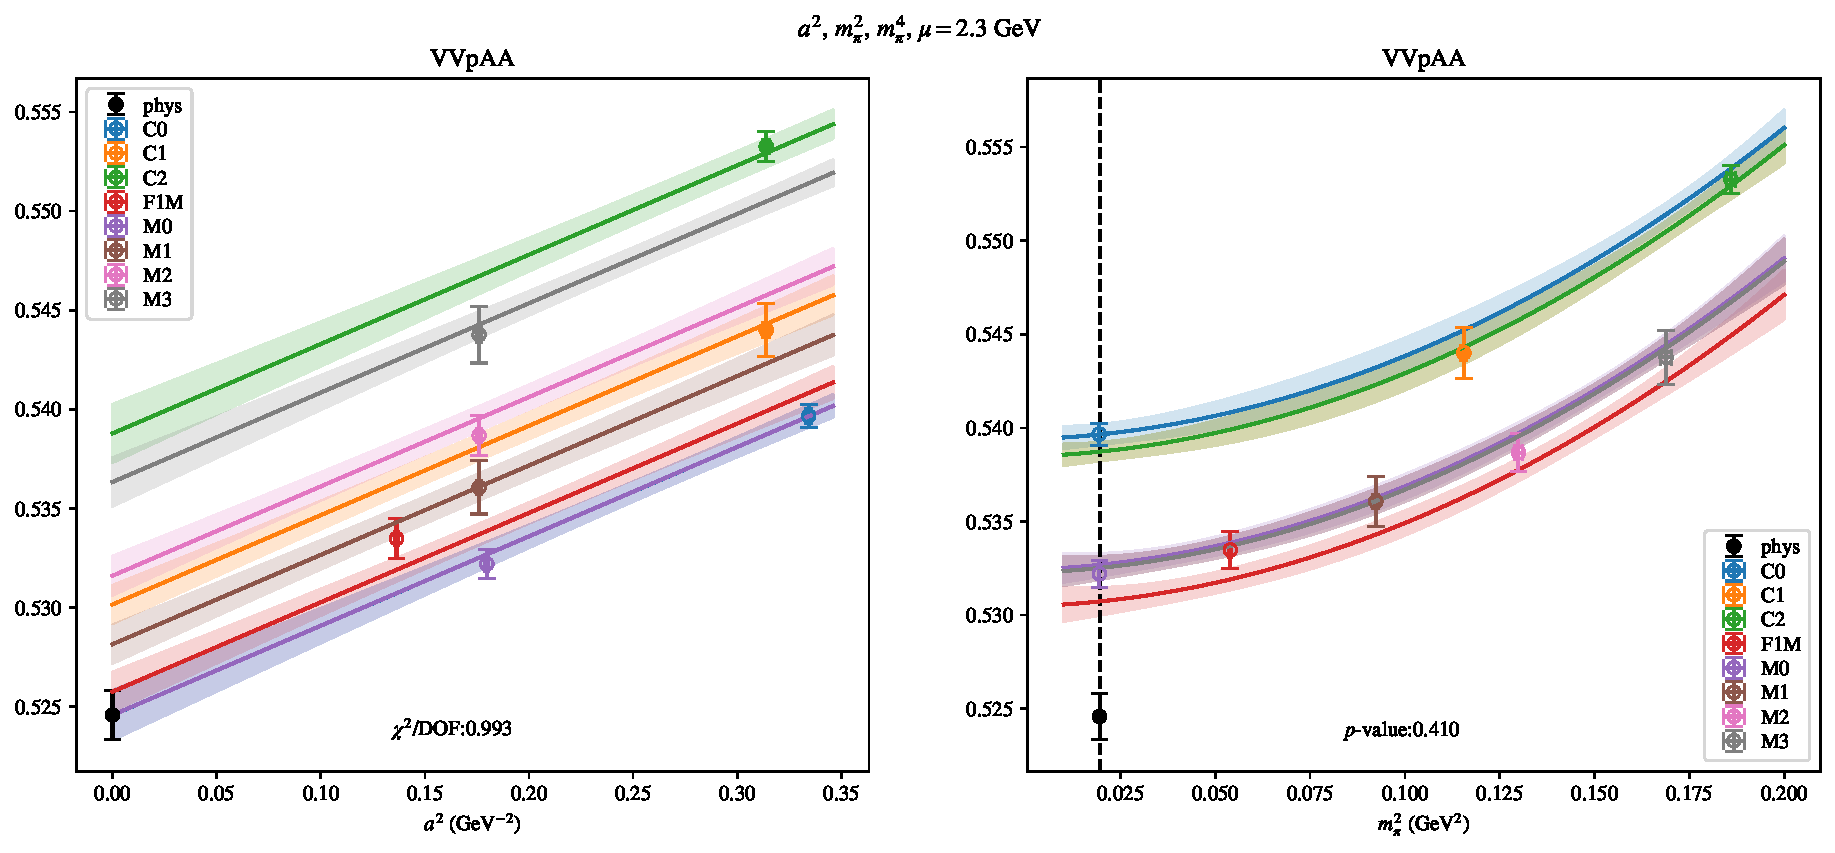
\includepdf[link, pages=-]{VVpAA/SUSY/a2m2m4_23.pdf}
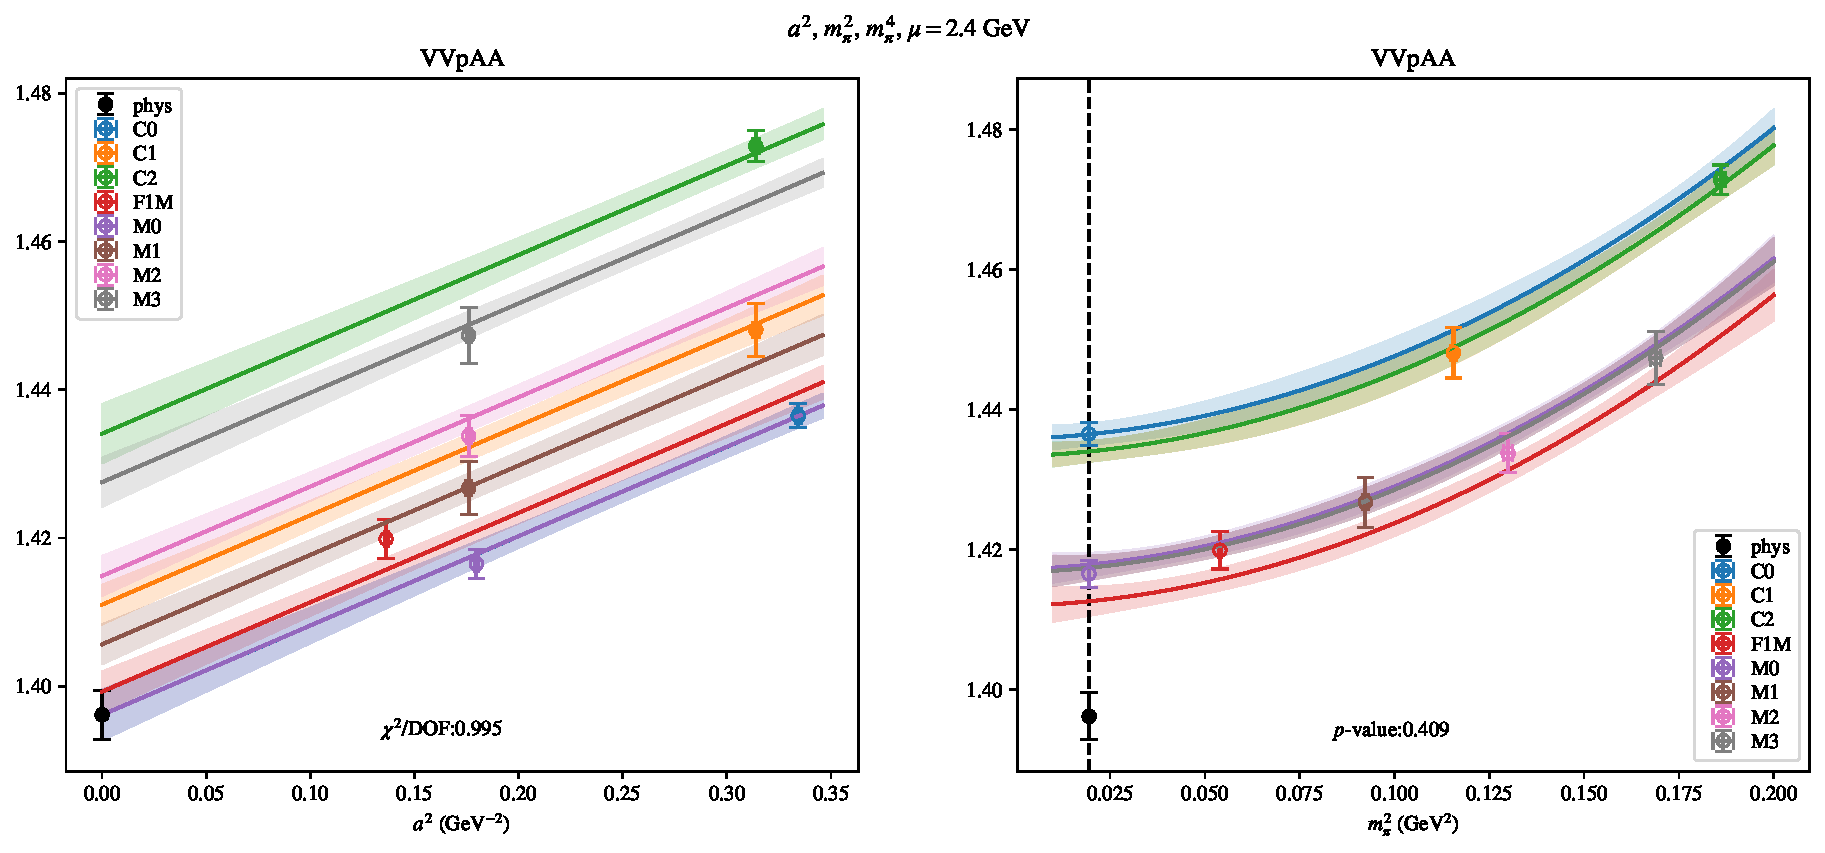
\includepdf[link, pages=-]{VVpAA/SUSY/a2m2m4_24.pdf}
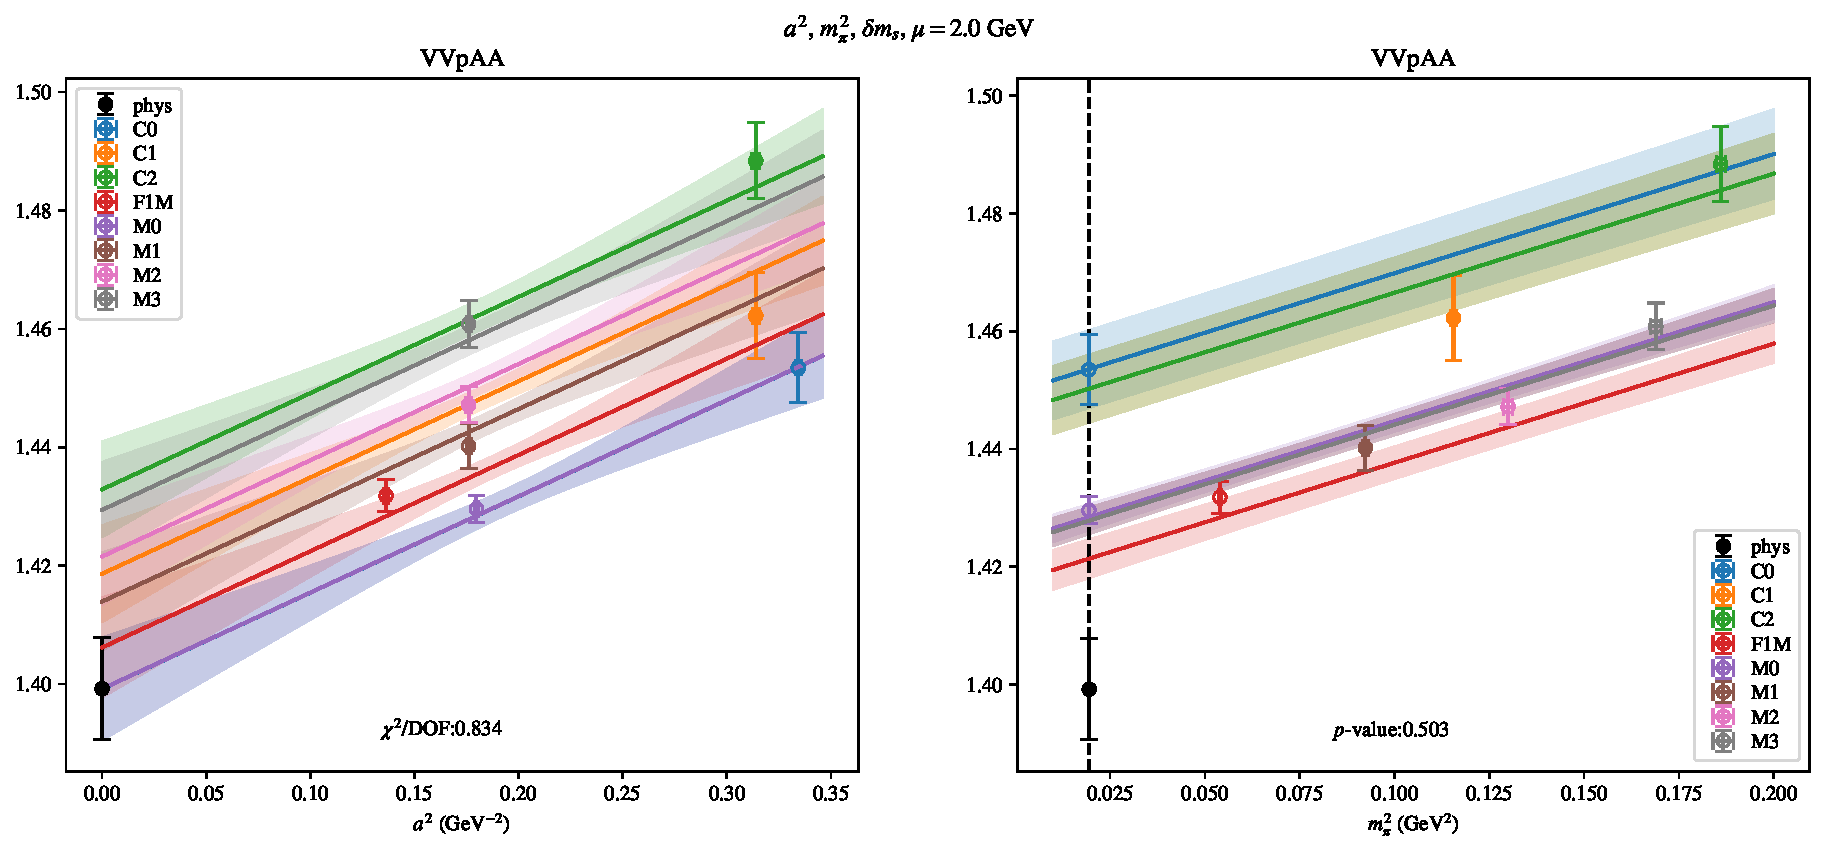
\includepdf[link, pages=-]{VVpAA/SUSY/a2m2delm_20.pdf}
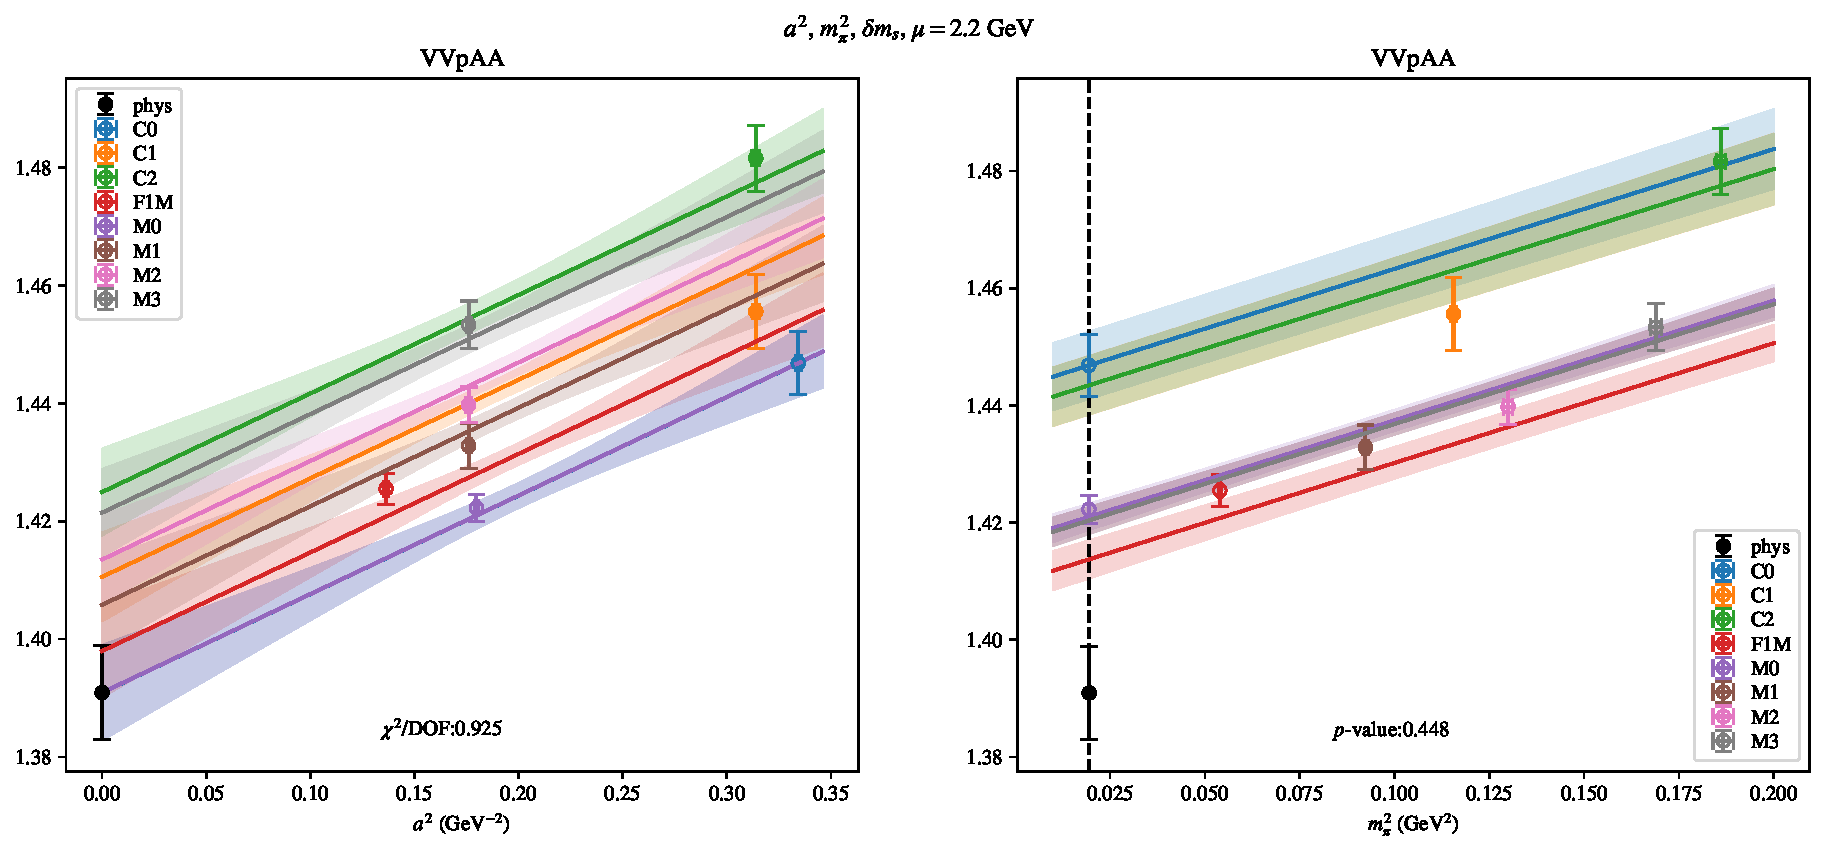
\includepdf[link, pages=-]{VVpAA/SUSY/a2m2delm_22.pdf}
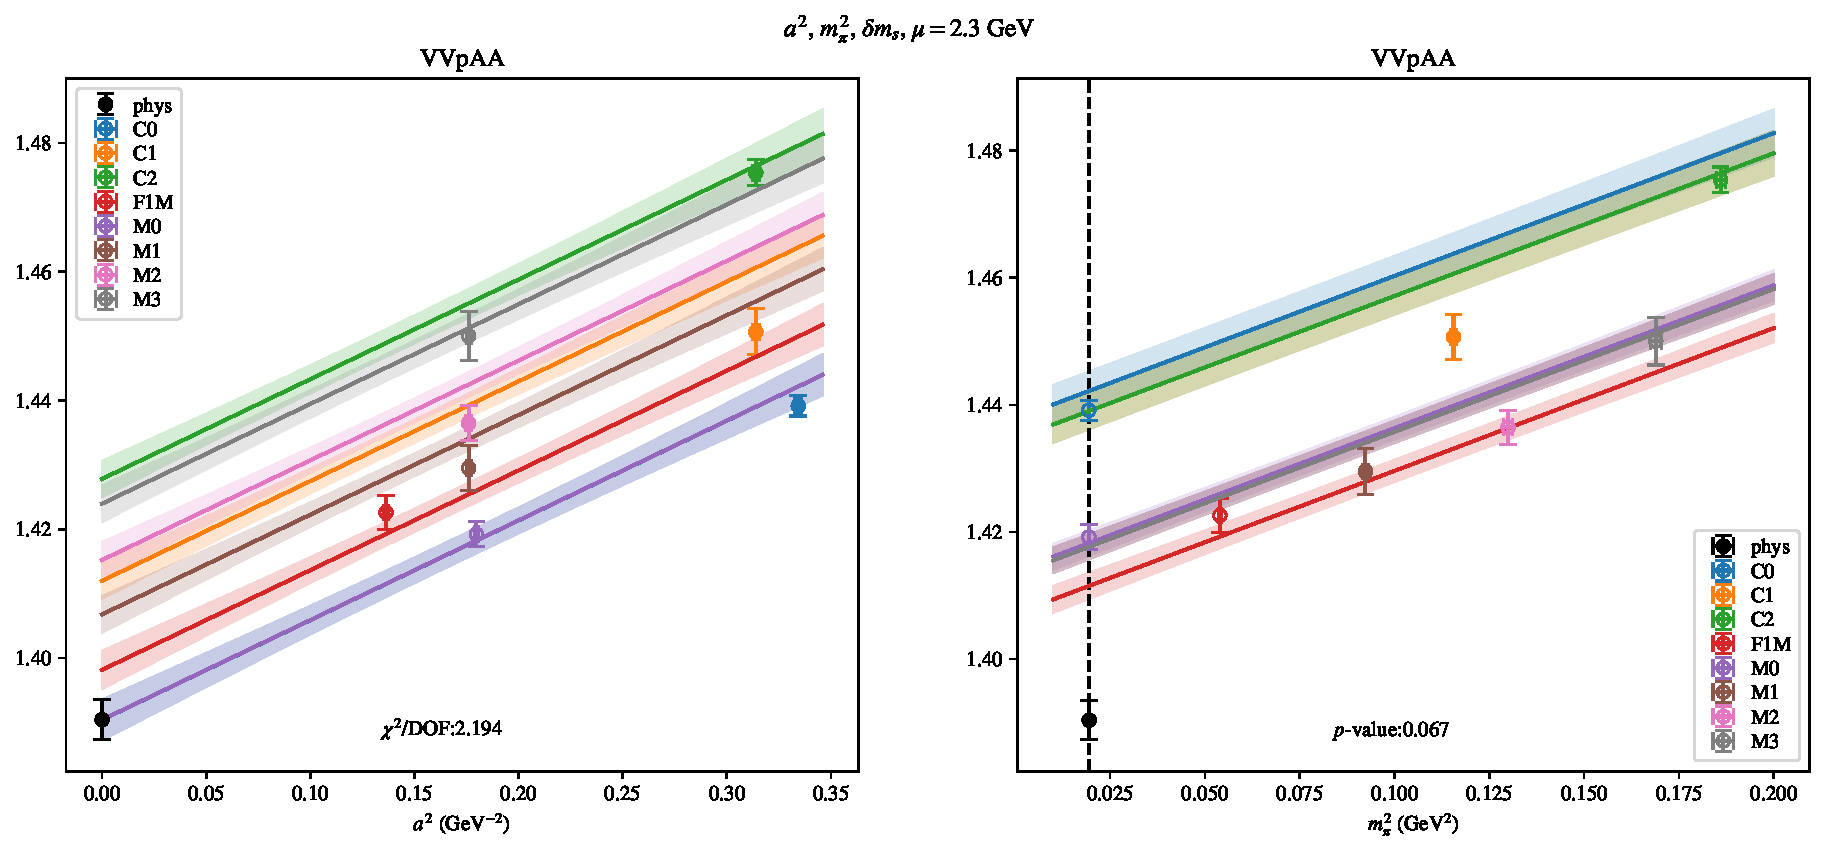
\includepdf[link, pages=-]{VVpAA/SUSY/a2m2delm_23.pdf}
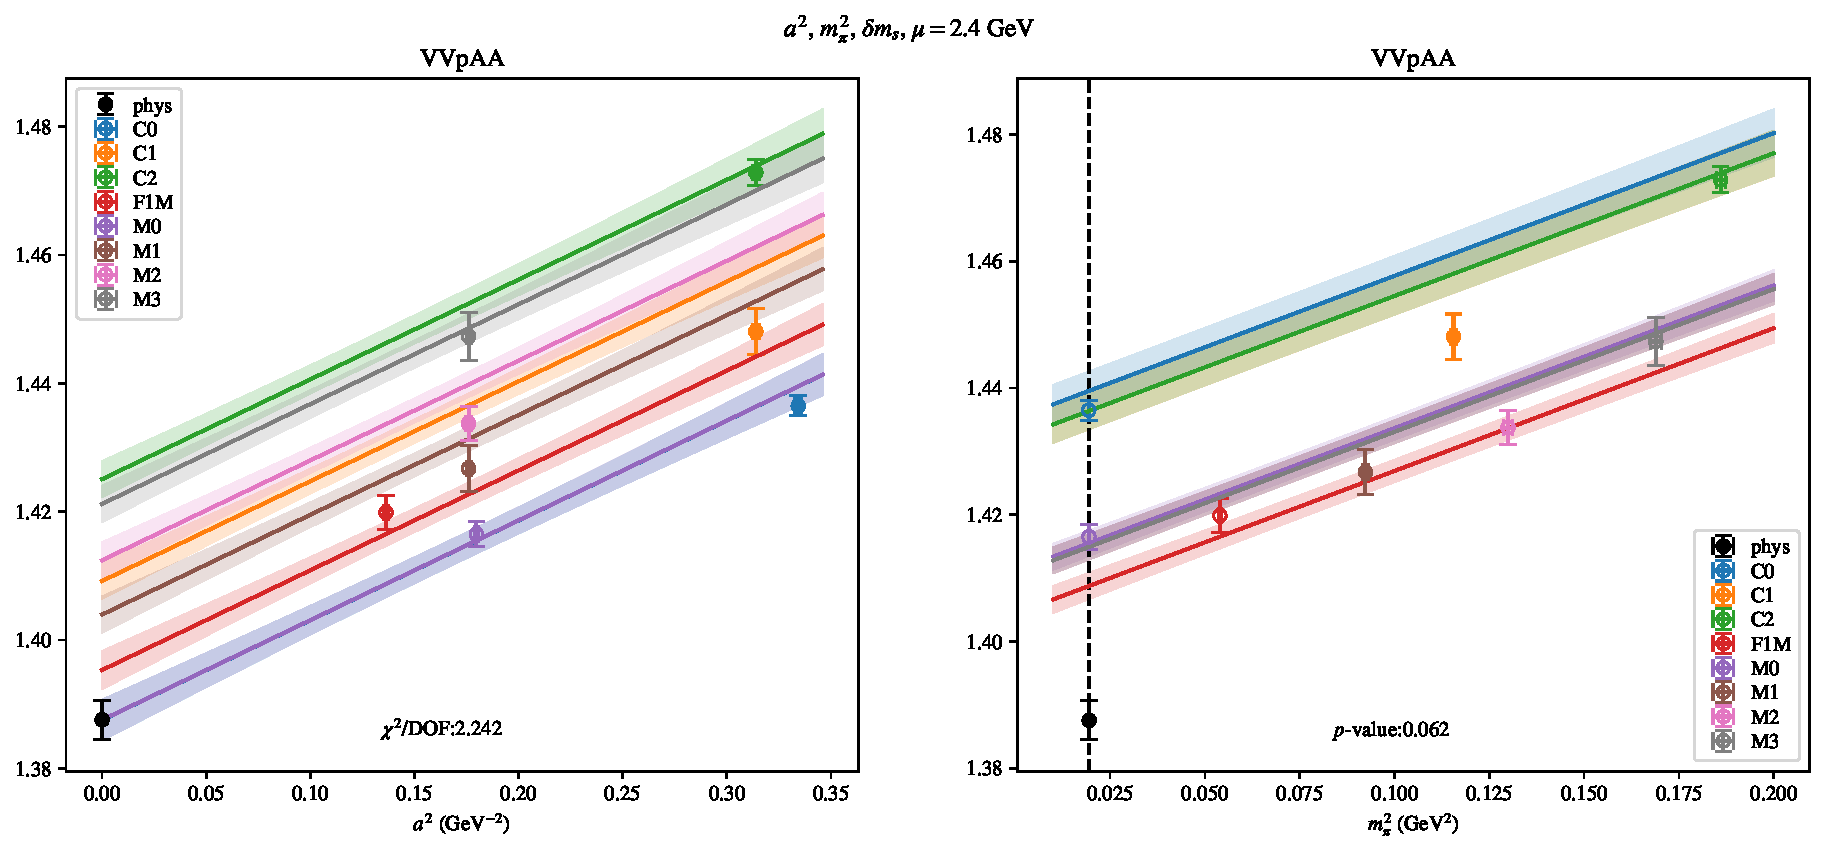
\includepdf[link, pages=-]{VVpAA/SUSY/a2m2delm_24.pdf}
\clearpage
\section{$\mathcal{B}_2$}
\begin{table}[h!]
\begin{center}
\begin{tabular}{|c|c|c|c|c|c|c|}
\hline
$\mu$ (GeV) & $a^2$, $m_\pi^2$& $a^2$, $m_\pi^2$ (no C)& $a^2$, $a^4$, $m_\pi^2$& $a^2$, $m_\pi^2$ (no M3, C2)& $a^2$, $m_\pi^2$, $m_\pi^4$& $a^2$, $m_\pi^2$, $\delta m_s$\\
\hline
2.0& \hyperlink{VVmAA/SUSY/a2m2_20.pdf.1}{\textbf{-0.925(58)}: 0.257 (0.937)} & \hyperlink{VVmAA/SUSY/a2m2noC_20.pdf.1}{\textbf{-0.91(17)}: 0.302 (0.74)} & \hyperlink{VVmAA/SUSY/a2a4m2_20.pdf.1}{\textbf{-0.89(54)}: 0.126 (0.973)} & \hyperlink{VVmAA/SUSY/a2m2mcut_20.pdf.1}{\textbf{-0.923(54)}: 0.35 (0.789)} & \hyperlink{VVmAA/SUSY/a2m2m4_20.pdf.1}{\textbf{-0.922(70)}: 0.269 (0.898)} & \hyperlink{VVmAA/SUSY/a2m2delm_20.pdf.1}{\textbf{-0.93(15)}: 0.157 (0.96)}\\
2.2& \hyperlink{VVmAA/SUSY/a2m2_22.pdf.1}{\textbf{-0.907(45)}: 0.534 (0.751)} & \hyperlink{VVmAA/SUSY/a2m2noC_22.pdf.1}{\textbf{-0.91(13)}: 0.593 (0.553)} & \hyperlink{VVmAA/SUSY/a2a4m2_22.pdf.1}{\textbf{-0.90(26)}: 0.617 (0.65)} & \hyperlink{VVmAA/SUSY/a2m2mcut_22.pdf.1}{\textbf{-0.907(44)}: 0.701 (0.551)} & \hyperlink{VVmAA/SUSY/a2m2m4_22.pdf.1}{\textbf{-0.904(50)}: 0.462 (0.764)} & \hyperlink{VVmAA/SUSY/a2m2delm_22.pdf.1}{\textbf{-0.906(78)}: 0.619 (0.649)}\\
2.3& \hyperlink{VVmAA/SUSY/a2m2_23.pdf.1}{\textbf{-0.898(48)}: 0.612 (0.69)} & \hyperlink{VVmAA/SUSY/a2m2noC_23.pdf.1}{\textbf{-0.90(11)}: 0.755 (0.47)} & \hyperlink{VVmAA/SUSY/a2a4m2_23.pdf.1}{\textbf{-0.90(25)}: 0.632 (0.64)} & \hyperlink{VVmAA/SUSY/a2m2mcut_23.pdf.1}{\textbf{-0.898(46)}: 0.896 (0.442)} & \hyperlink{VVmAA/SUSY/a2m2m4_23.pdf.1}{\textbf{-0.895(55)}: 0.512 (0.727)} & \hyperlink{VVmAA/SUSY/a2m2delm_23.pdf.1}{\textbf{-0.895(72)}: 0.659 (0.62)}\\
2.4& \hyperlink{VVmAA/SUSY/a2m2_24.pdf.1}{\textbf{-0.890(51)}: 0.617 (0.687)} & \hyperlink{VVmAA/SUSY/a2m2noC_24.pdf.1}{\textbf{-0.89(11)}: 0.925 (0.397)} & \hyperlink{VVmAA/SUSY/a2a4m2_24.pdf.1}{\textbf{-0.90(23)}: 0.749 (0.559)} & \hyperlink{VVmAA/SUSY/a2m2mcut_24.pdf.1}{\textbf{-0.891(50)}: 0.804 (0.491)} & \hyperlink{VVmAA/SUSY/a2m2m4_24.pdf.1}{\textbf{-0.887(53)}: 0.541 (0.706)} & \hyperlink{VVmAA/SUSY/a2m2delm_24.pdf.1}{\textbf{-0.888(77)}: 0.629 (0.642)}\\
\hline
\end{tabular}
\caption{Physical point value from chiral and continuum extrapolation at renormalisation scale $\mu$. Entries are \textbf{value(error)}: $\chi^2/\text{DOF}$ ($p$-value).}
\end{center}
\end{table}
\begin{table}[h!]
\begin{center}
\begin{tabular}{|c c|c|c|c|c|c|c|}
\hline
$\mu$ (GeV) &  & $a^2$, $m_\pi^2$& $a^2$, $m_\pi^2$ (no C)& $a^2$, $a^4$, $m_\pi^2$& $a^2$, $m_\pi^2$ (no M3, C2)& $a^2$, $m_\pi^2$, $m_\pi^4$& $a^2$, $m_\pi^2$, $\delta m_s$\\
\hline
\multirow{2}{0.5in}{2.0} & $\alpha$ & 0.395(37)& 0.50(14)& 0.73(71)& 0.400(34)& 0.403(42)& 0.373(67)\\
 & $\beta$ & 0.00707(37)& 0.00674(31)& 0.00695(22)& 0.00748(53)& 0.00834(89)& 0.00676(39)\\
\hline
\multirow{2}{0.5in}{2.2} & $\alpha$ & 0.431(27)& 0.41(10)& 0.40(31)& 0.429(25)& 0.439(27)& 0.435(37)\\
 & $\beta$ & 0.00687(19)& 0.00662(25)& 0.00690(20)& 0.00718(31)& 0.00850(84)& 0.00696(23)\\
\hline
\multirow{2}{0.5in}{2.3} & $\alpha$ & 0.457(30)& 0.418(90)& 0.35(30)& 0.454(29)& 0.467(35)& 0.467(39)\\
 & $\beta$ & 0.00683(21)& 0.00664(25)& 0.00681(22)& 0.00705(31)& 0.00828(95)& 0.00695(23)\\
\hline
\multirow{2}{0.5in}{2.4} & $\alpha$ & 0.476(33)& 0.429(84)& 0.36(26)& 0.471(33)& 0.487(34)& 0.488(43)\\
 & $\beta$ & 0.00686(21)& 0.00667(24)& 0.00687(22)& 0.00706(33)& 0.00861(94)& 0.00699(24)\\
\hline
\end{tabular}
\caption{Fit values of coefficients in $Q = Q_{phys} + \mathbf{\alpha} a^2 + \mathbf{\beta}\left(\frac{m_\pi^2}{f_\pi^2}-\frac{m_{\pi,PDG}^2}{f_\pi^2}\right) + \ldots$.}
\end{center}
\end{table}
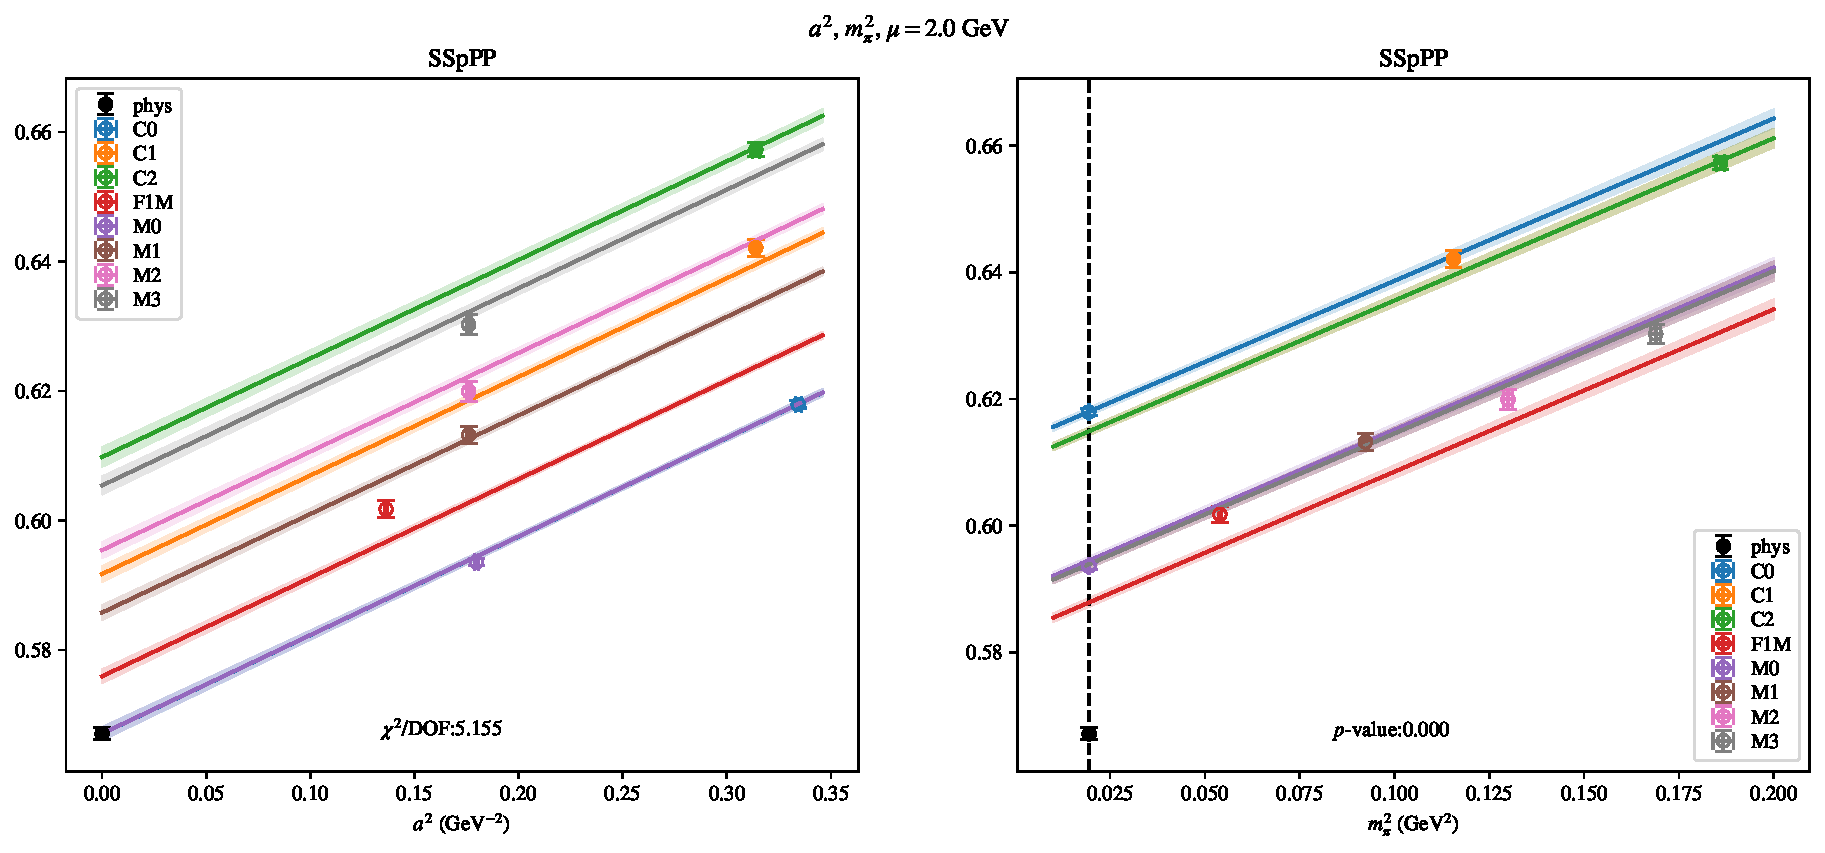
\includepdf[link, pages=-]{VVmAA/SUSY/a2m2_20.pdf}
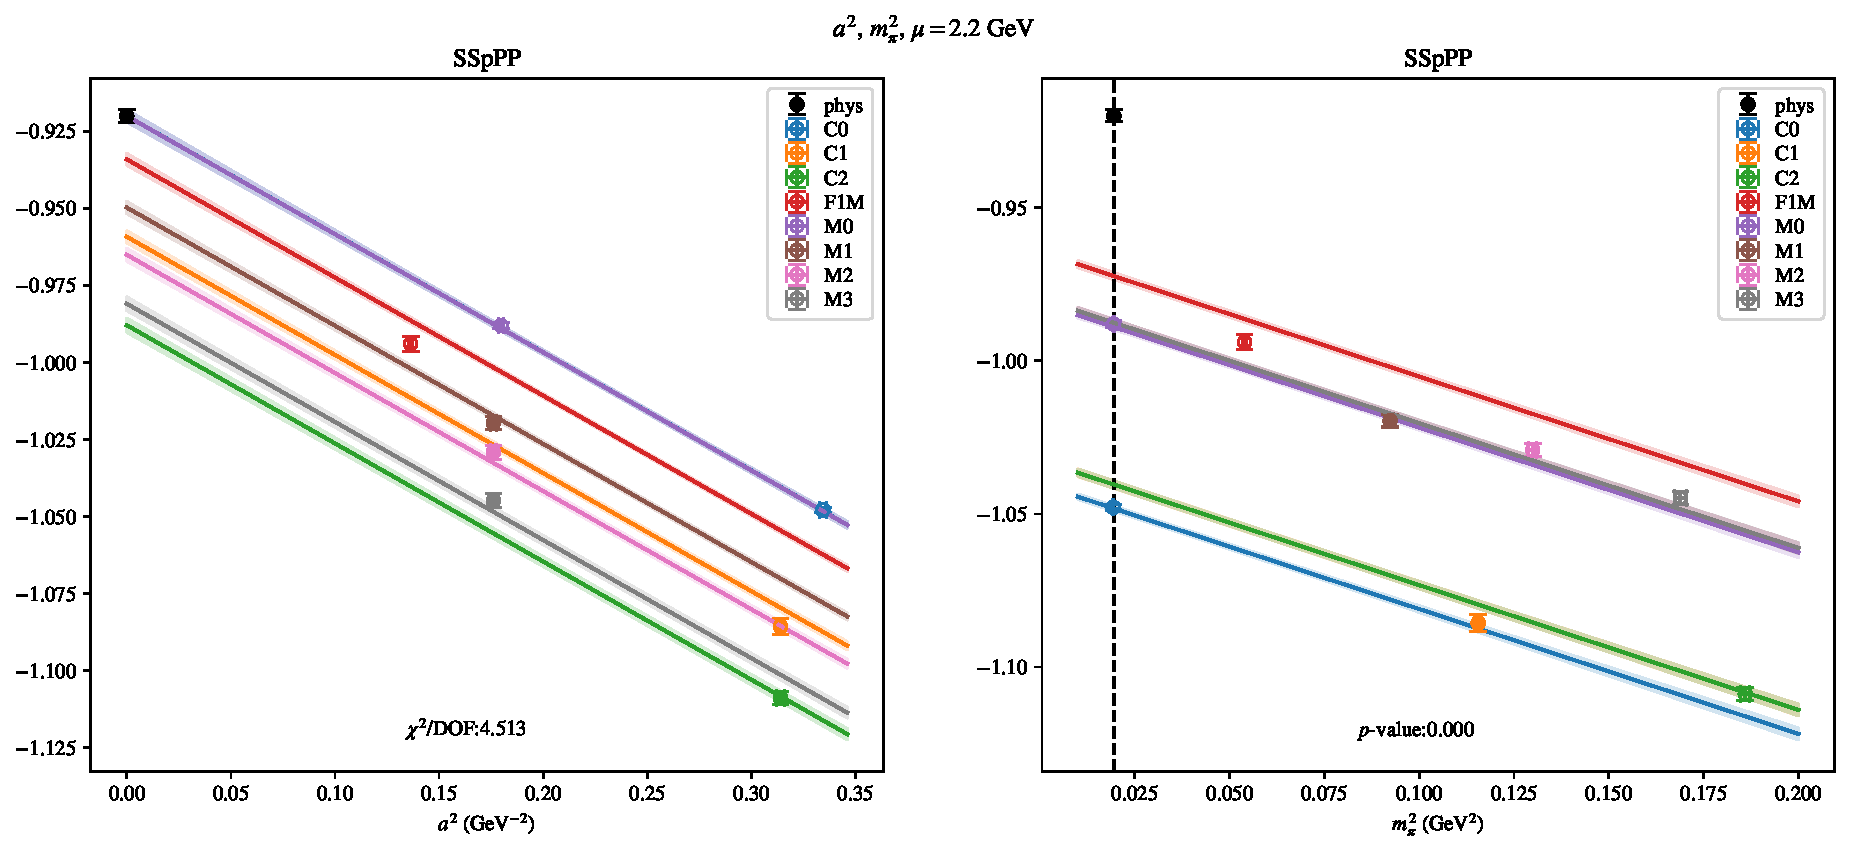
\includepdf[link, pages=-]{VVmAA/SUSY/a2m2_22.pdf}
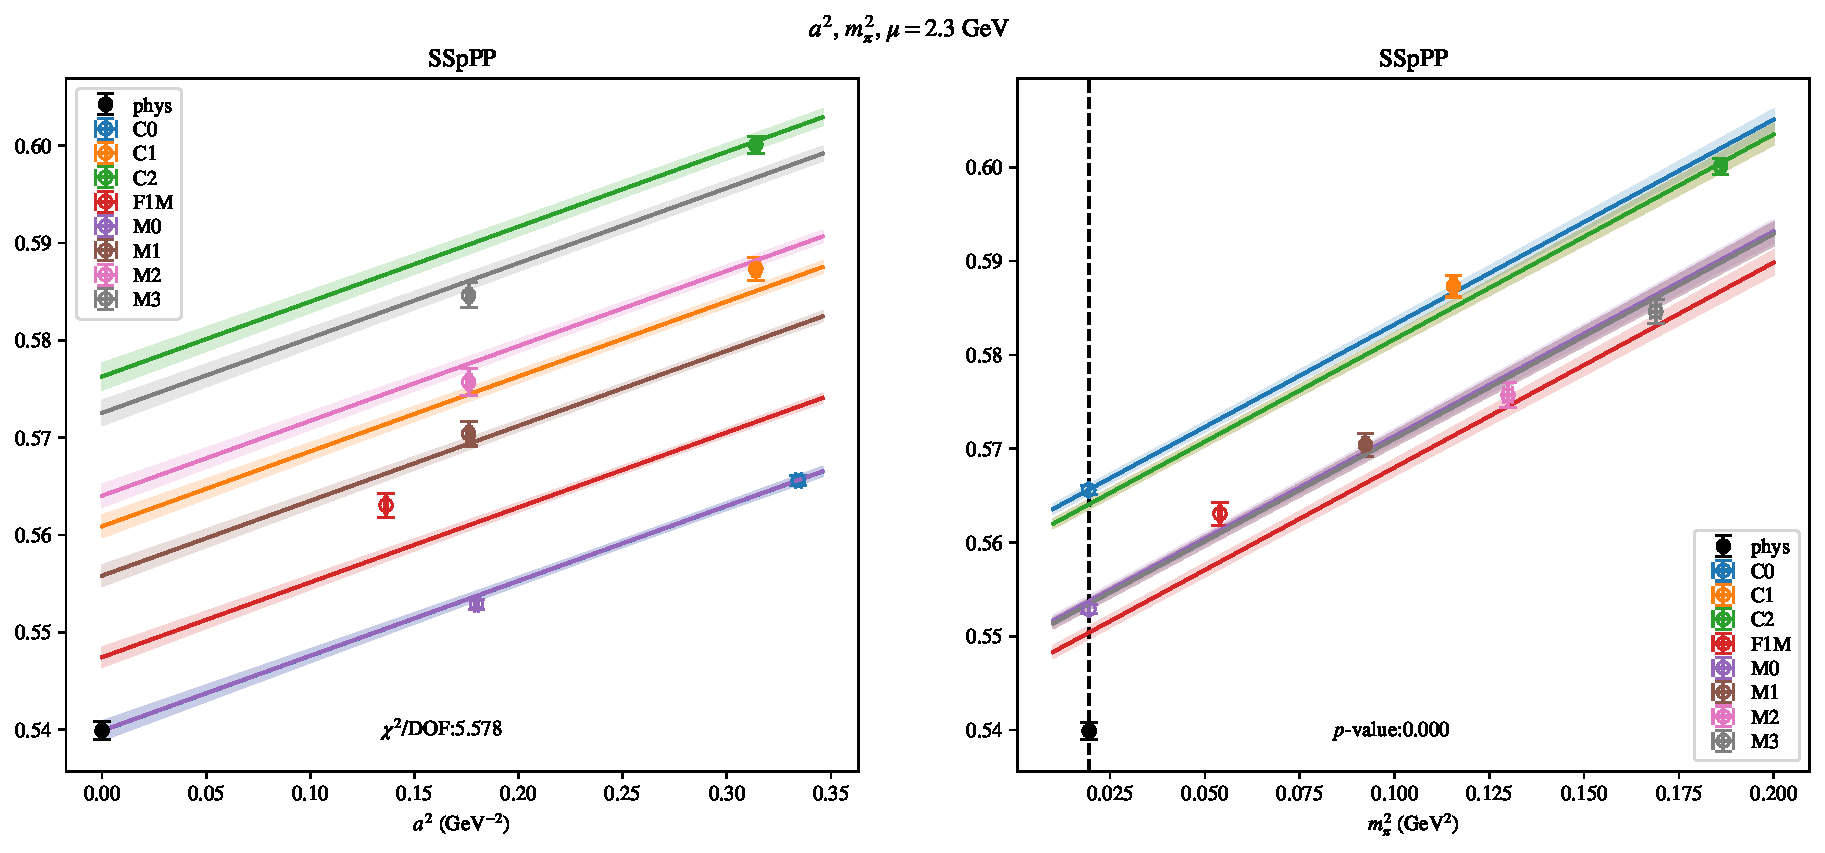
\includepdf[link, pages=-]{VVmAA/SUSY/a2m2_23.pdf}
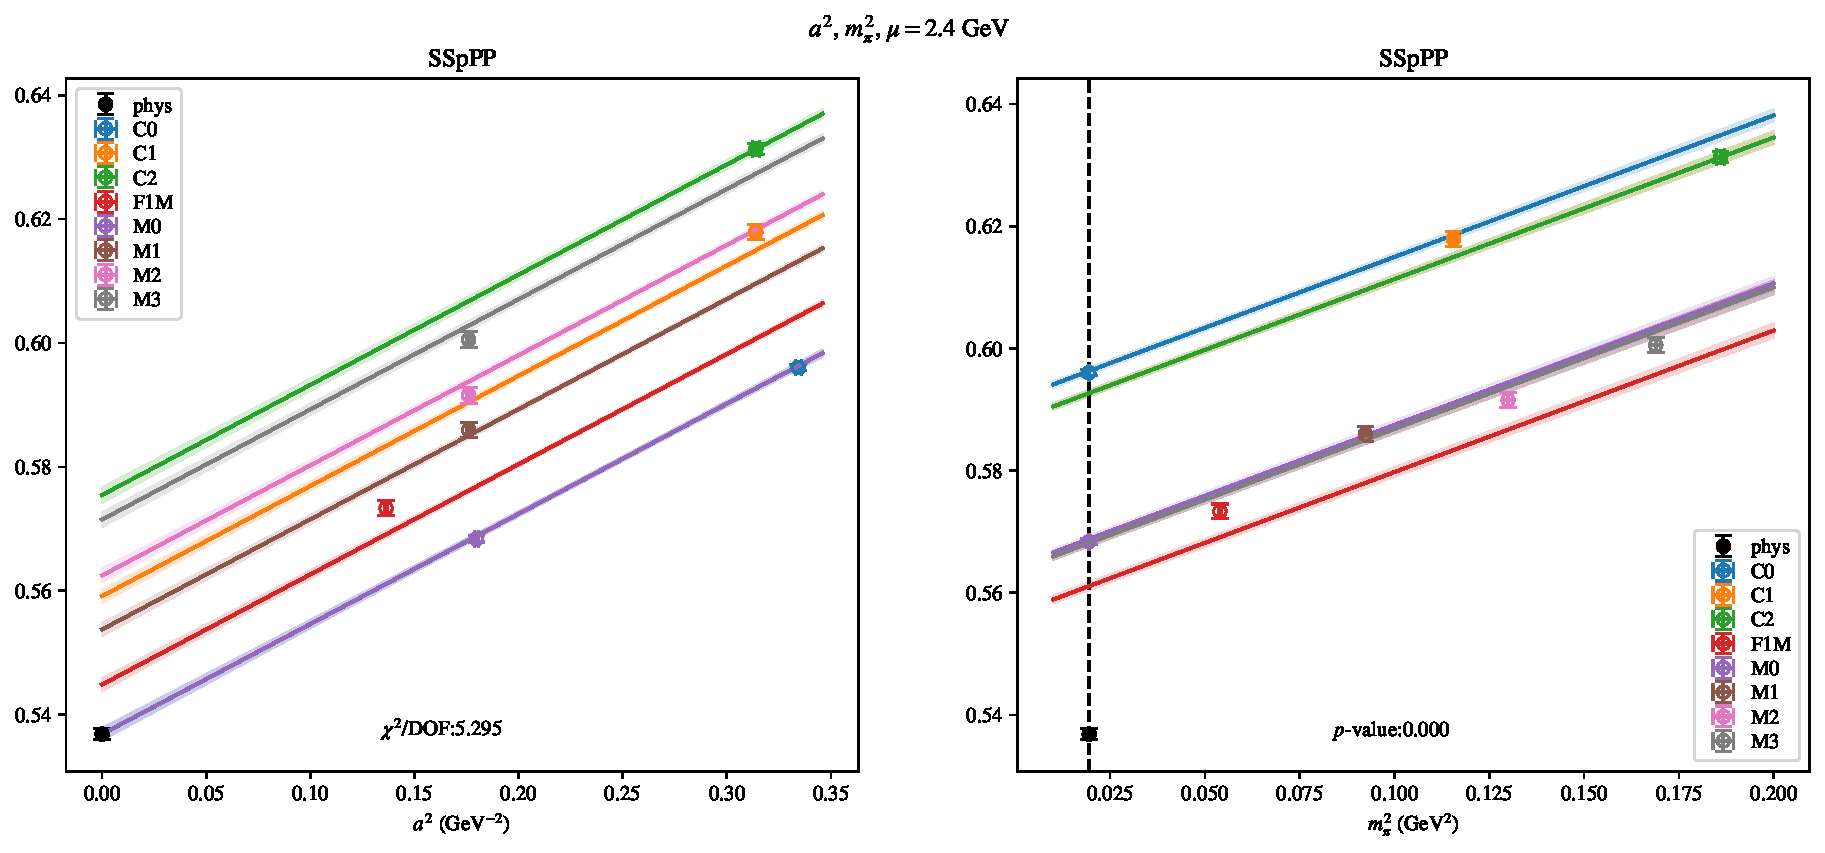
\includepdf[link, pages=-]{VVmAA/SUSY/a2m2_24.pdf}
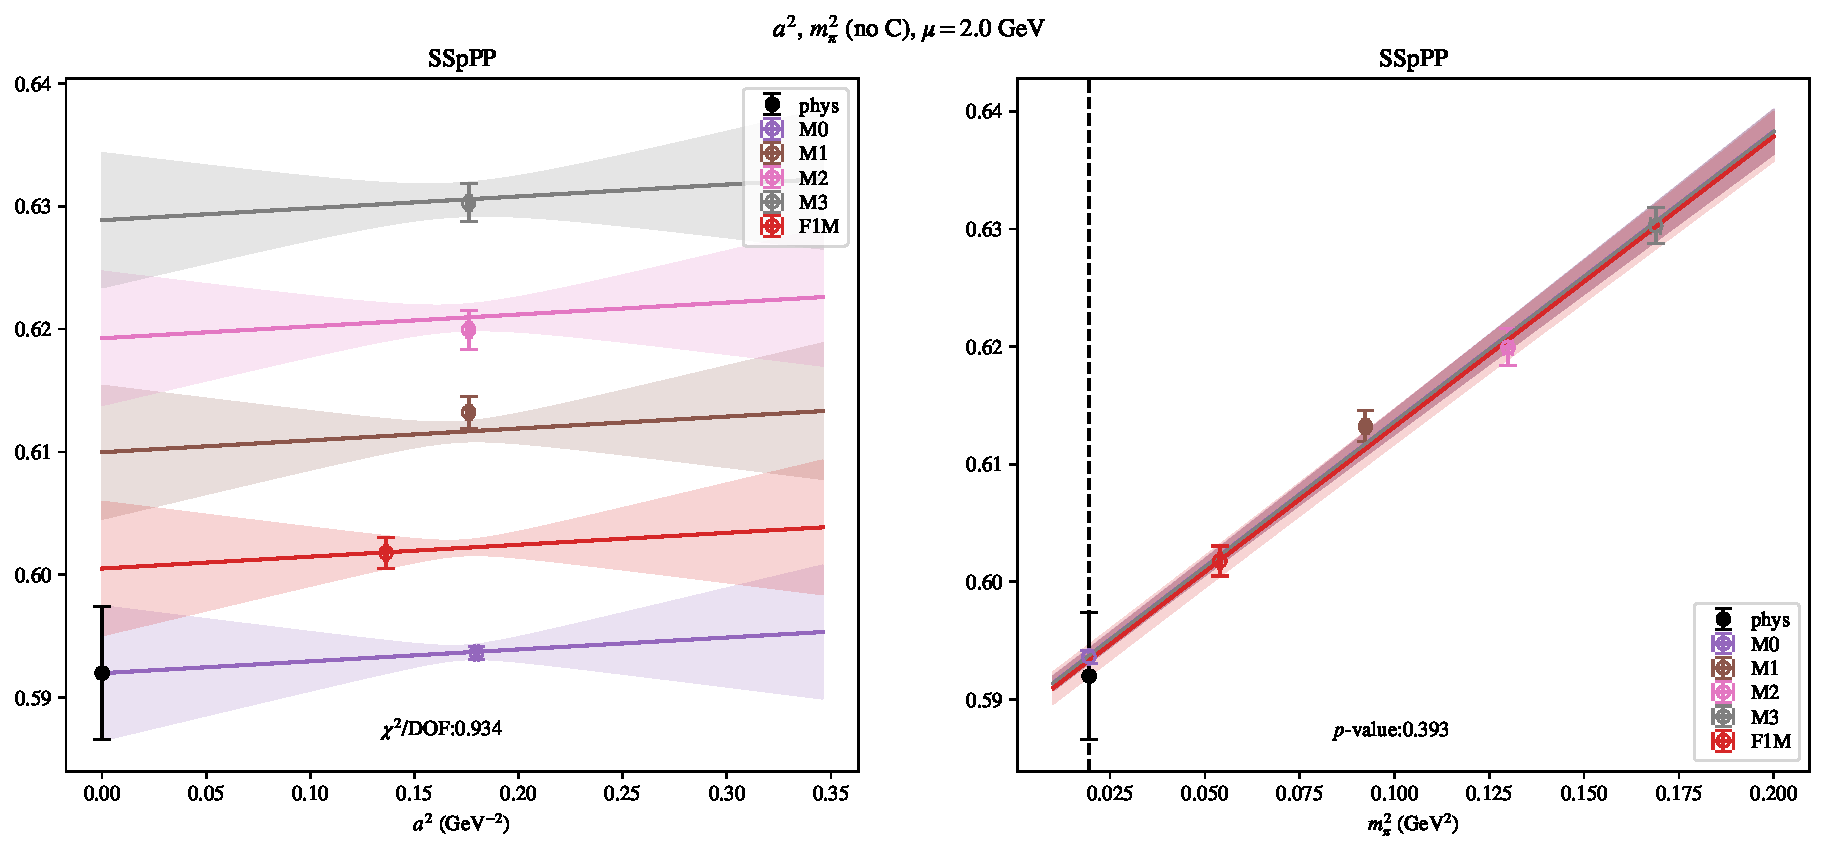
\includepdf[link, pages=-]{VVmAA/SUSY/a2m2noC_20.pdf}
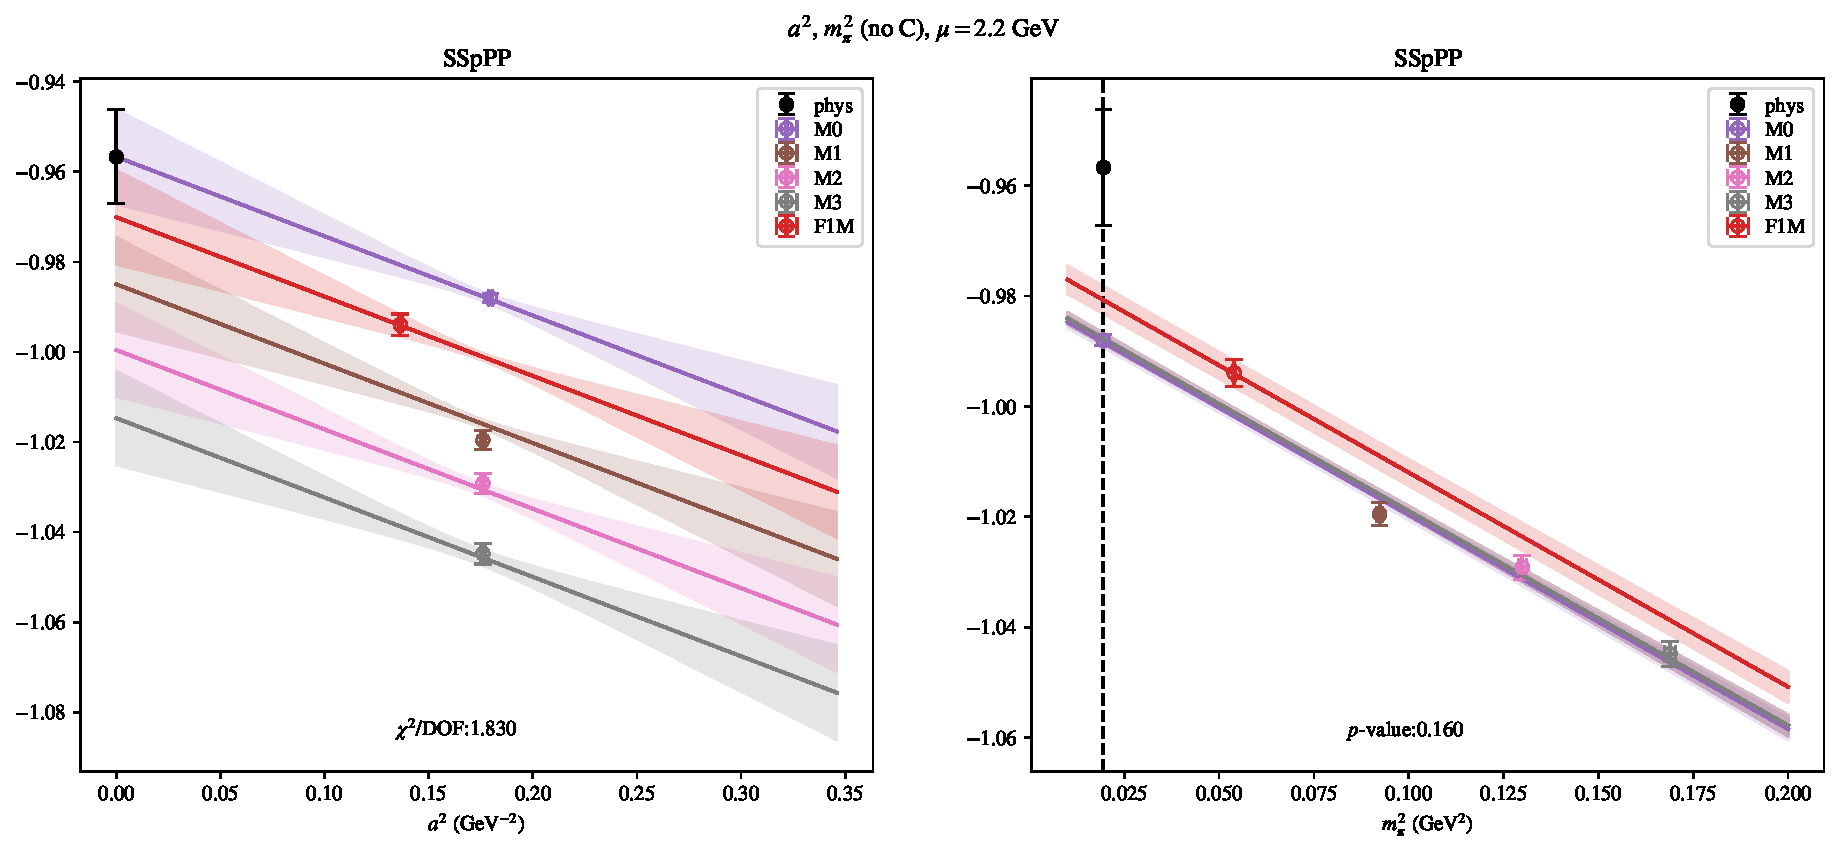
\includepdf[link, pages=-]{VVmAA/SUSY/a2m2noC_22.pdf}
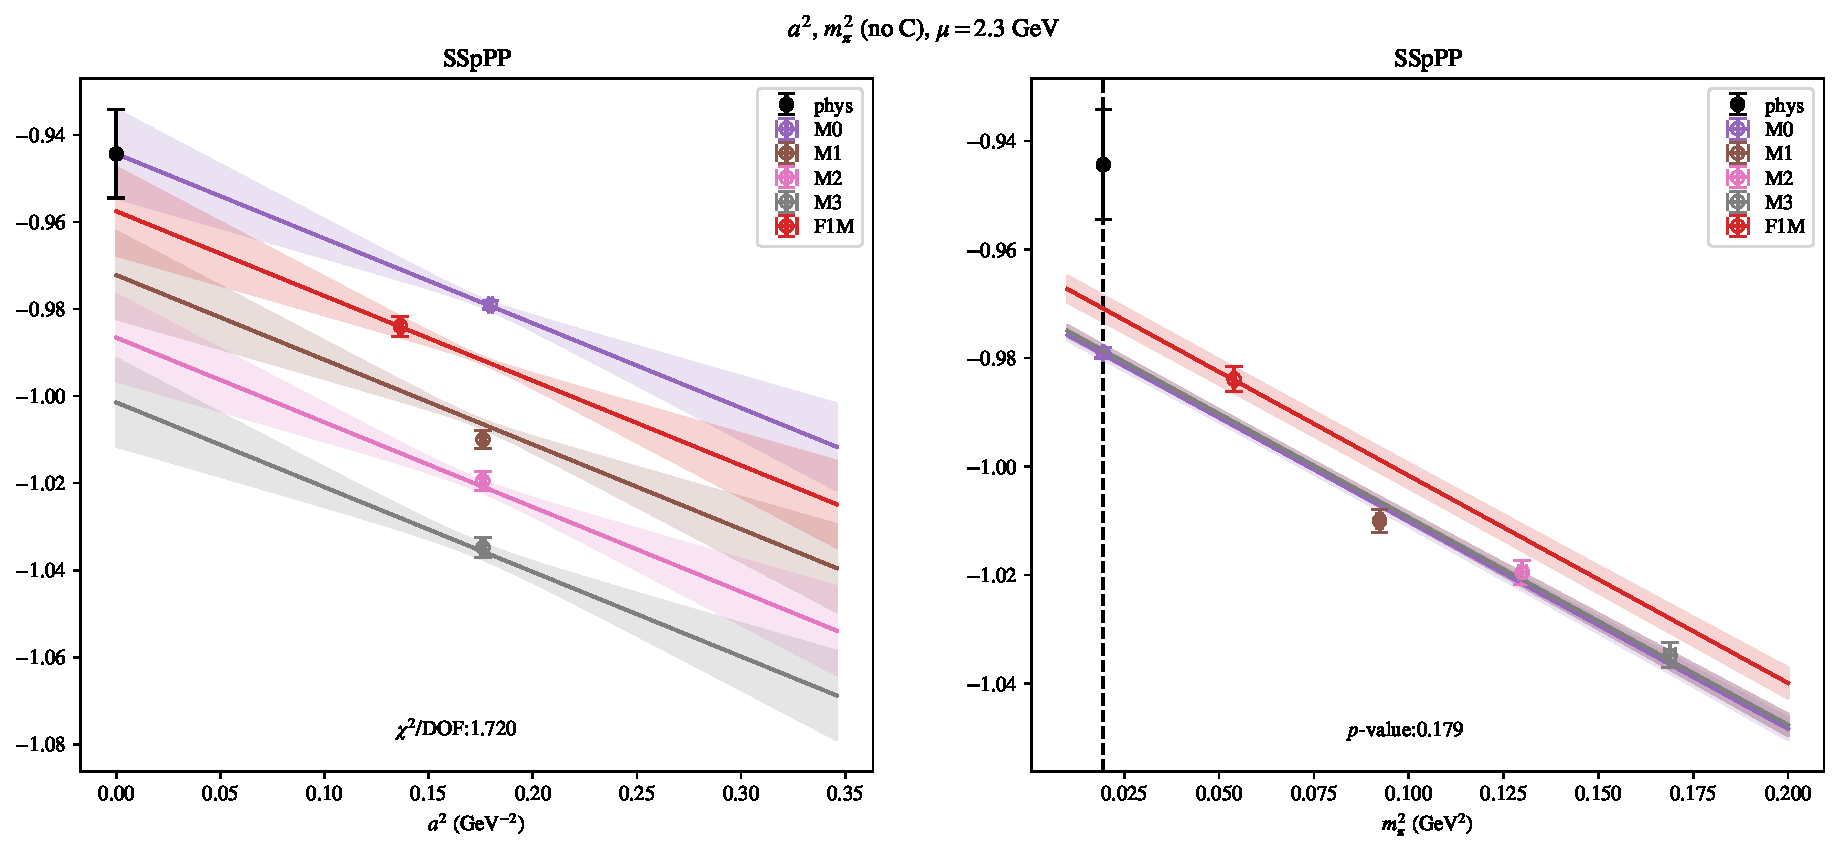
\includepdf[link, pages=-]{VVmAA/SUSY/a2m2noC_23.pdf}
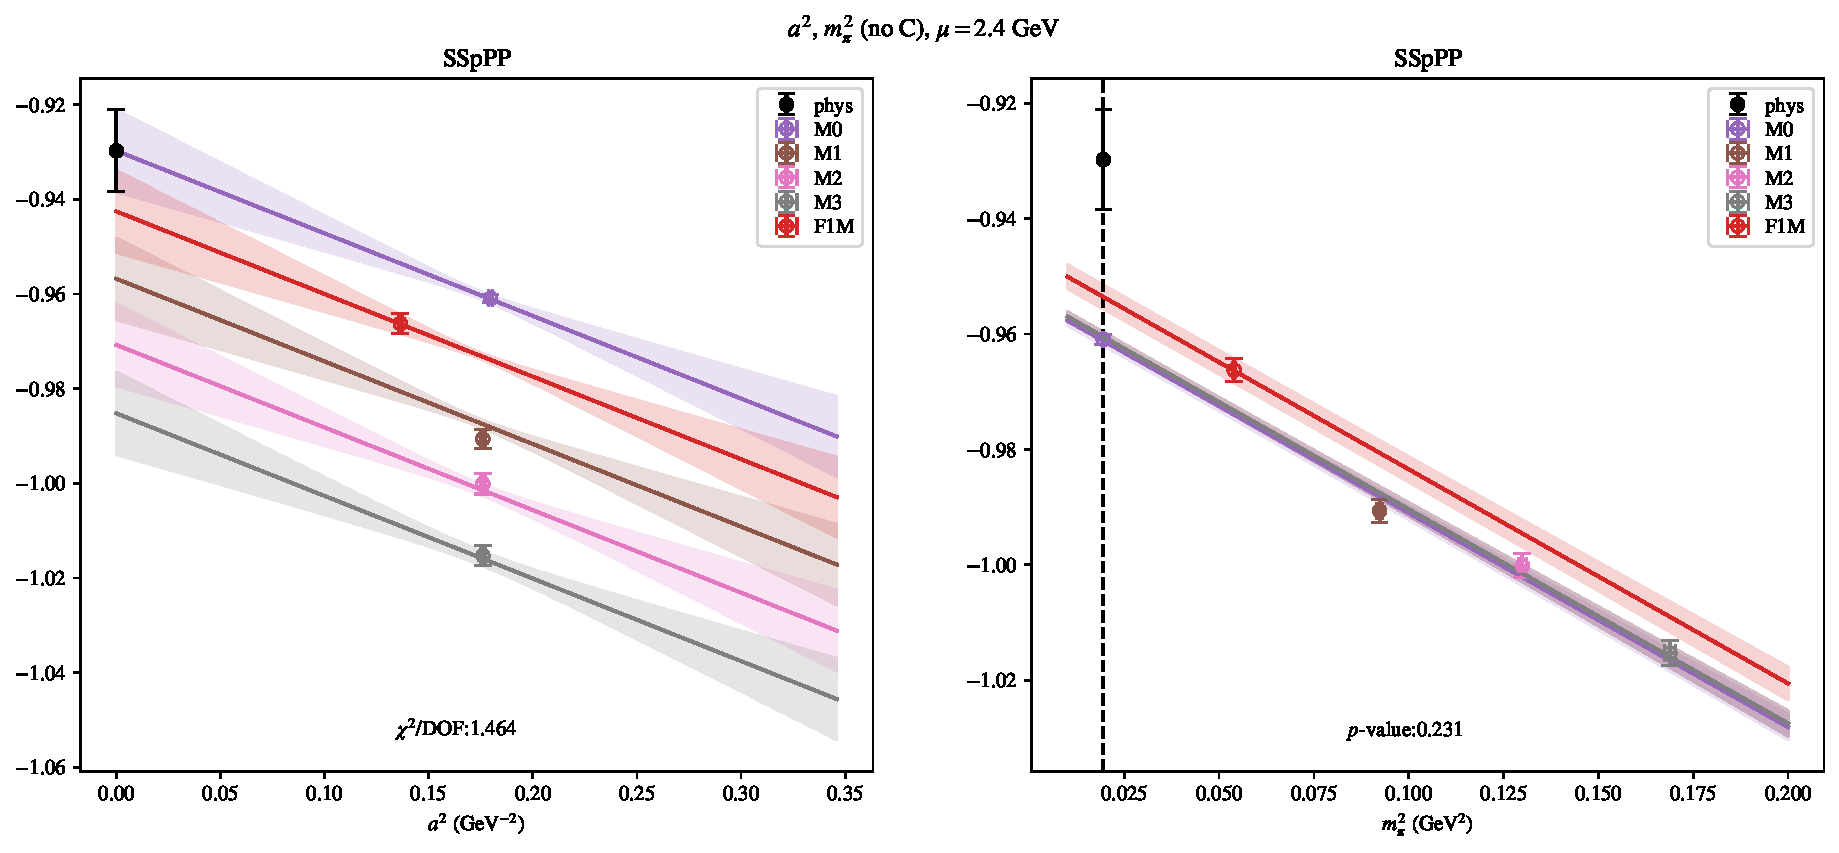
\includepdf[link, pages=-]{VVmAA/SUSY/a2m2noC_24.pdf}
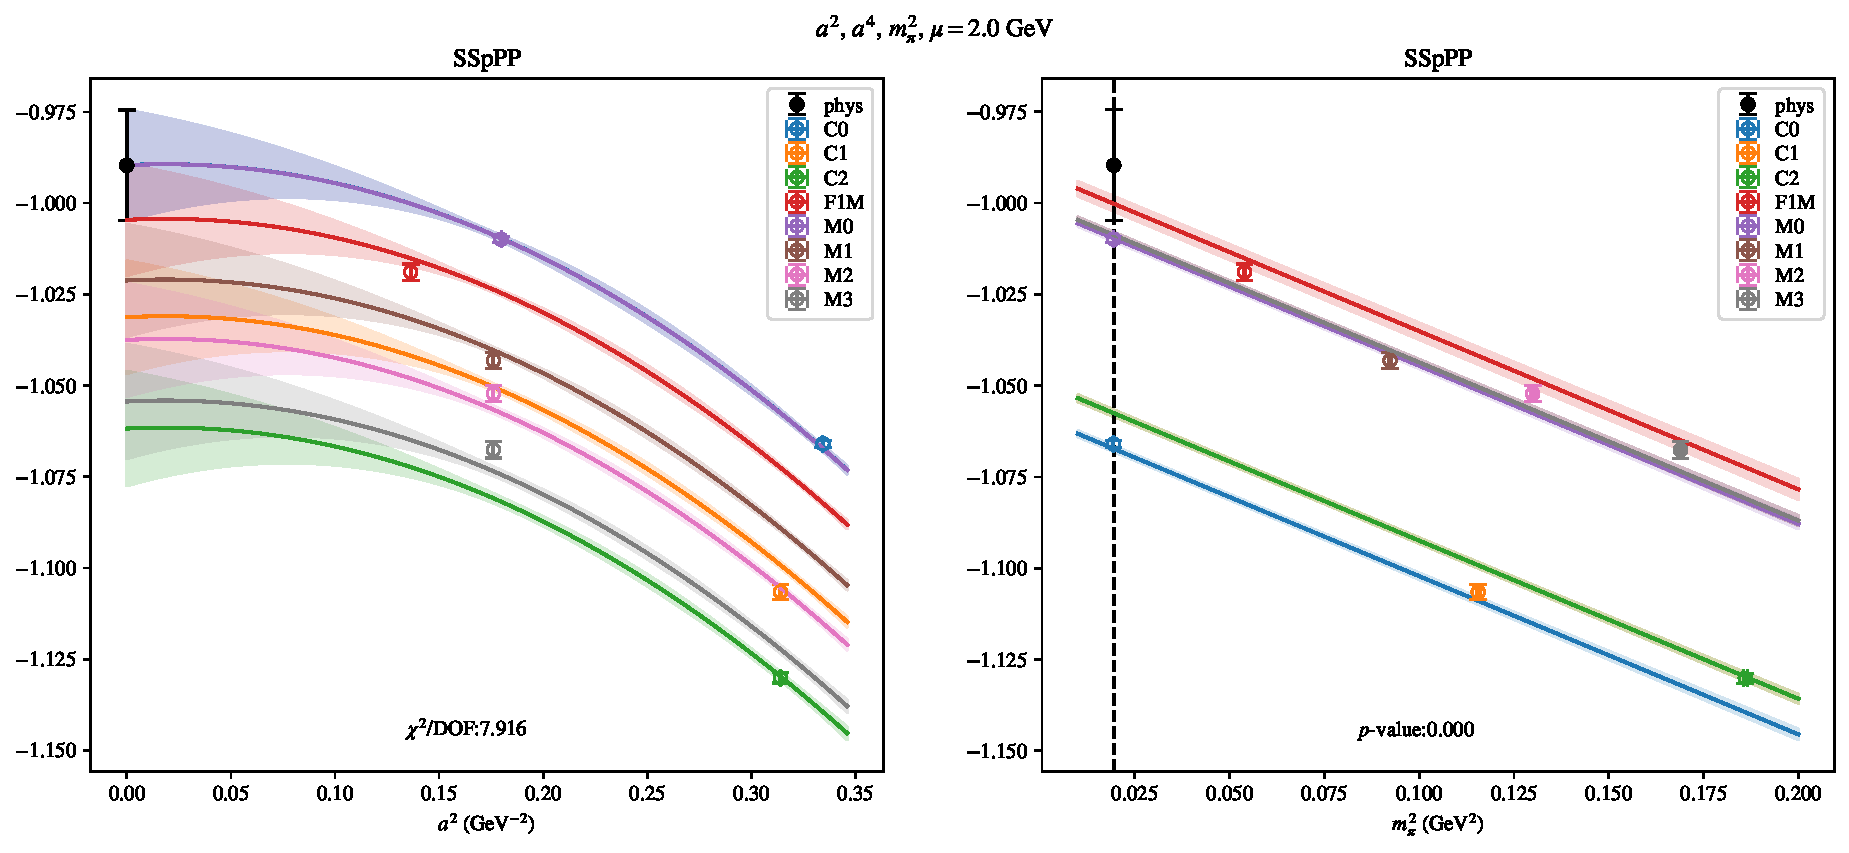
\includepdf[link, pages=-]{VVmAA/SUSY/a2a4m2_20.pdf}
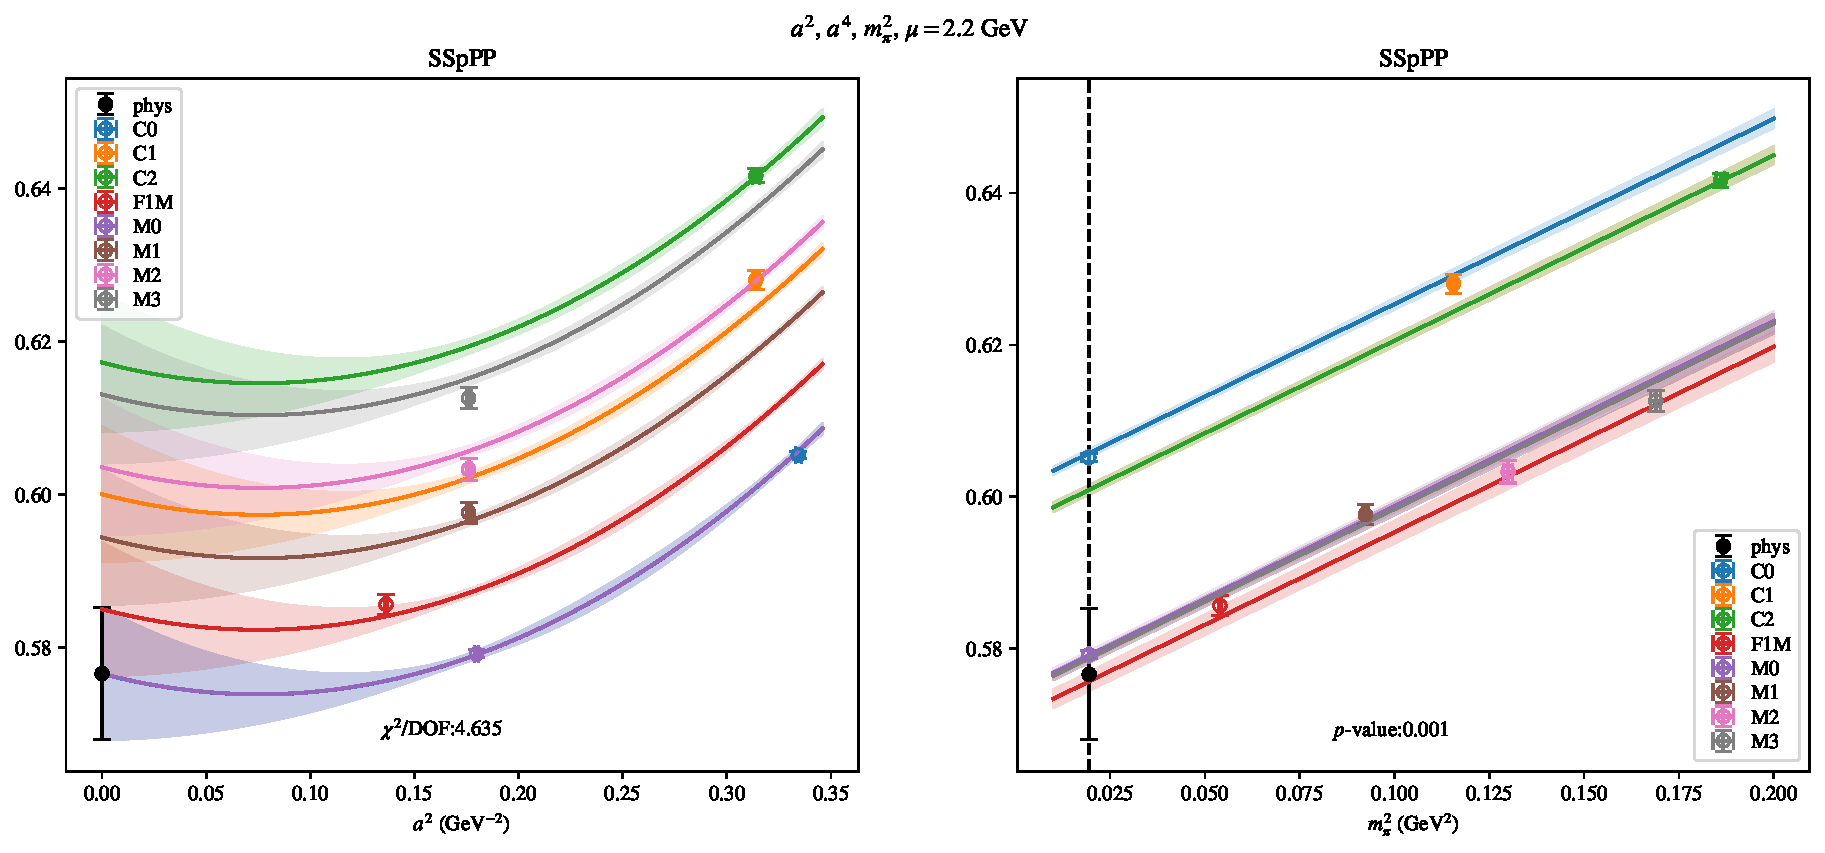
\includepdf[link, pages=-]{VVmAA/SUSY/a2a4m2_22.pdf}
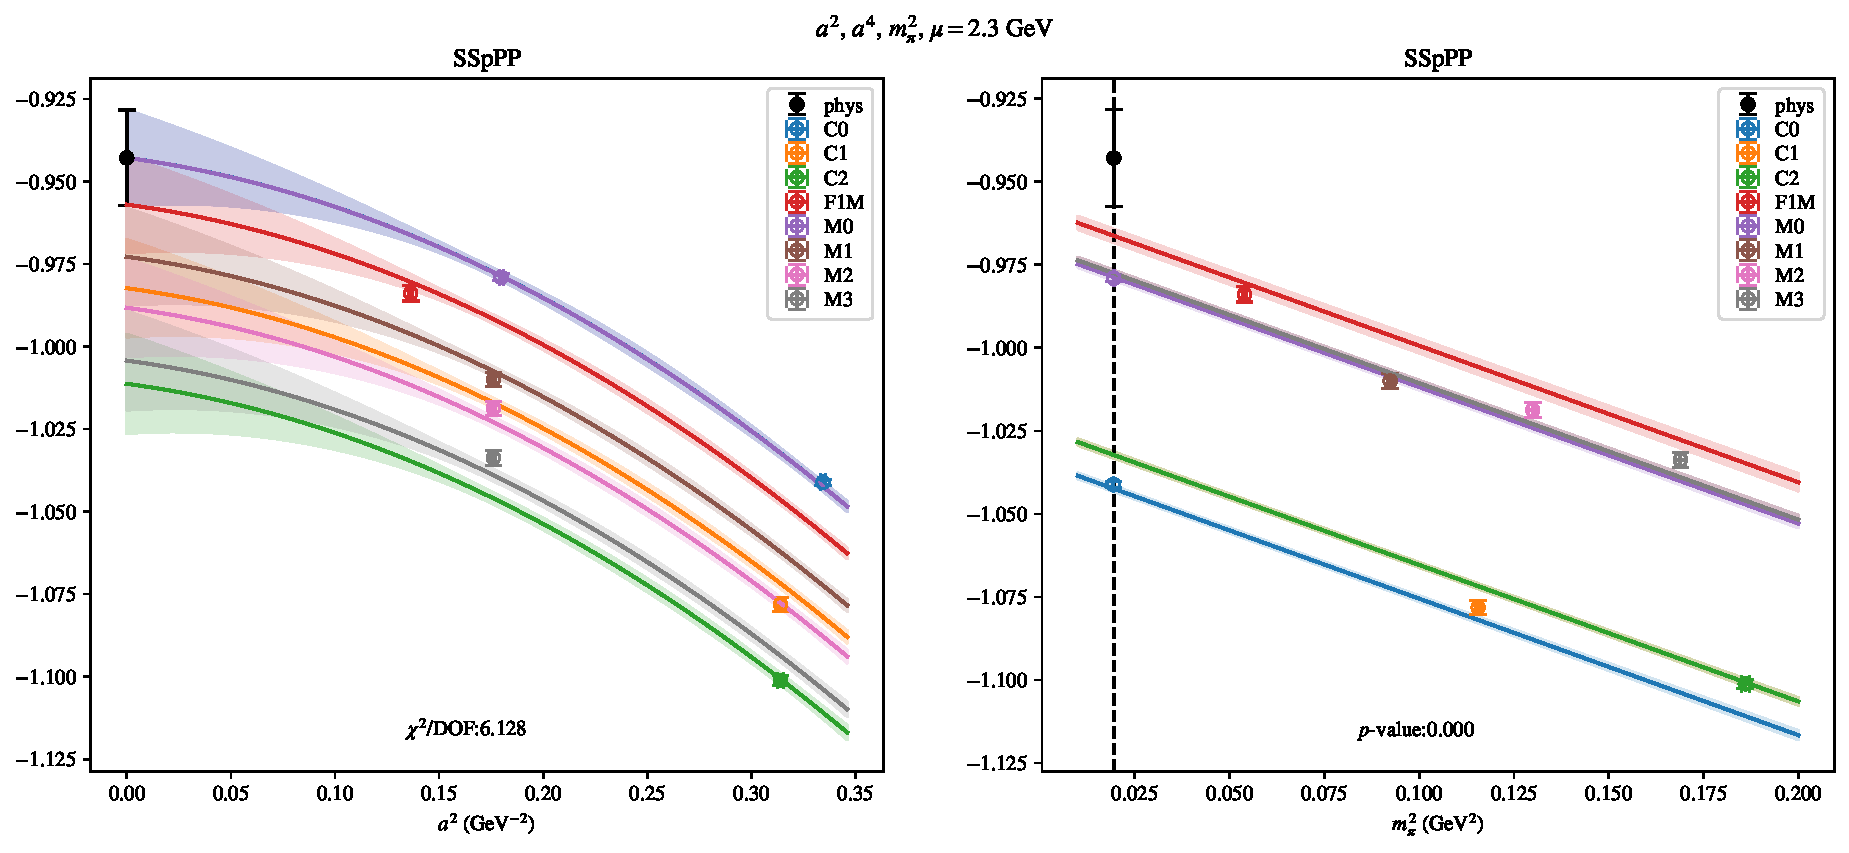
\includepdf[link, pages=-]{VVmAA/SUSY/a2a4m2_23.pdf}
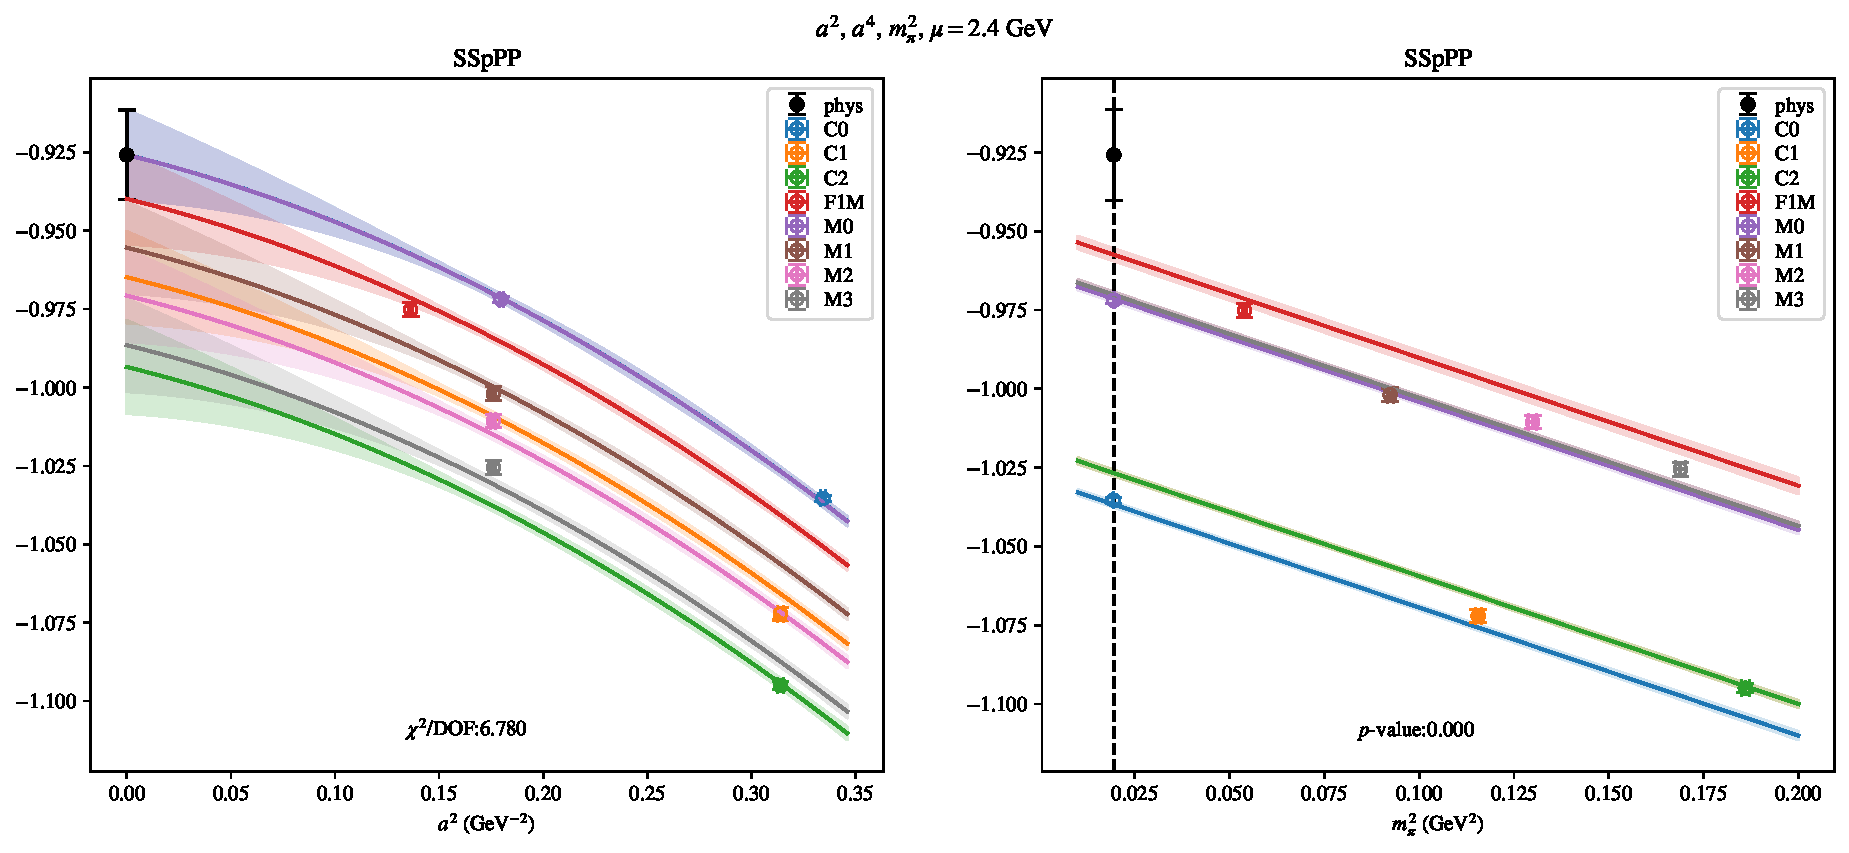
\includepdf[link, pages=-]{VVmAA/SUSY/a2a4m2_24.pdf}
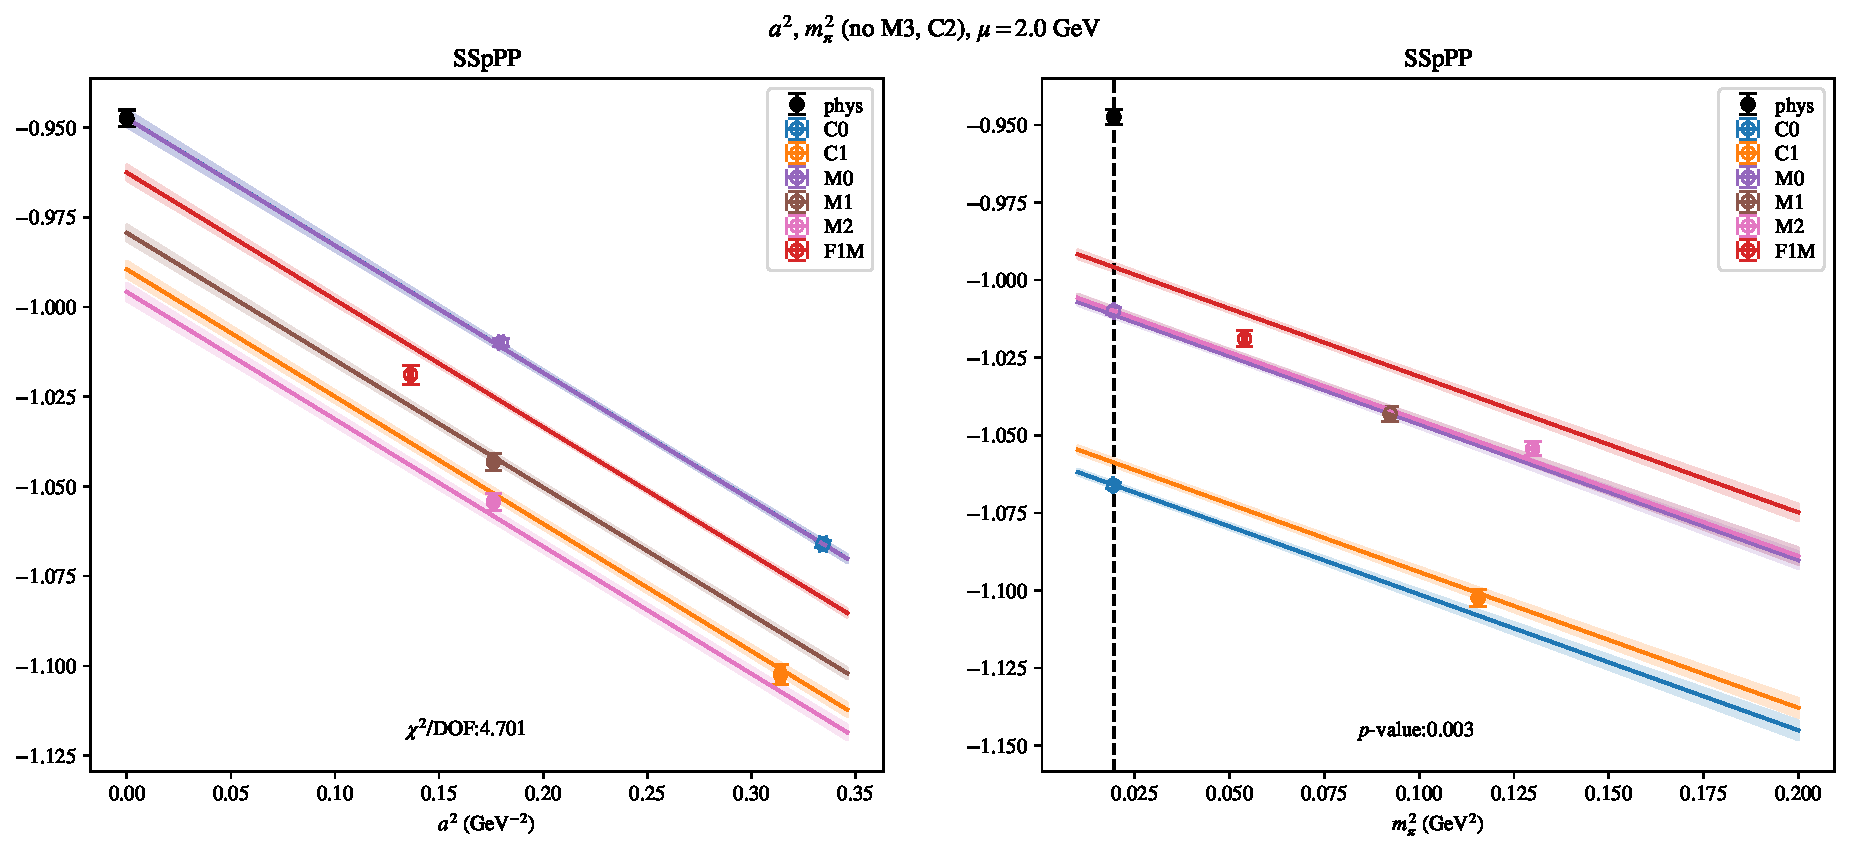
\includepdf[link, pages=-]{VVmAA/SUSY/a2m2mcut_20.pdf}
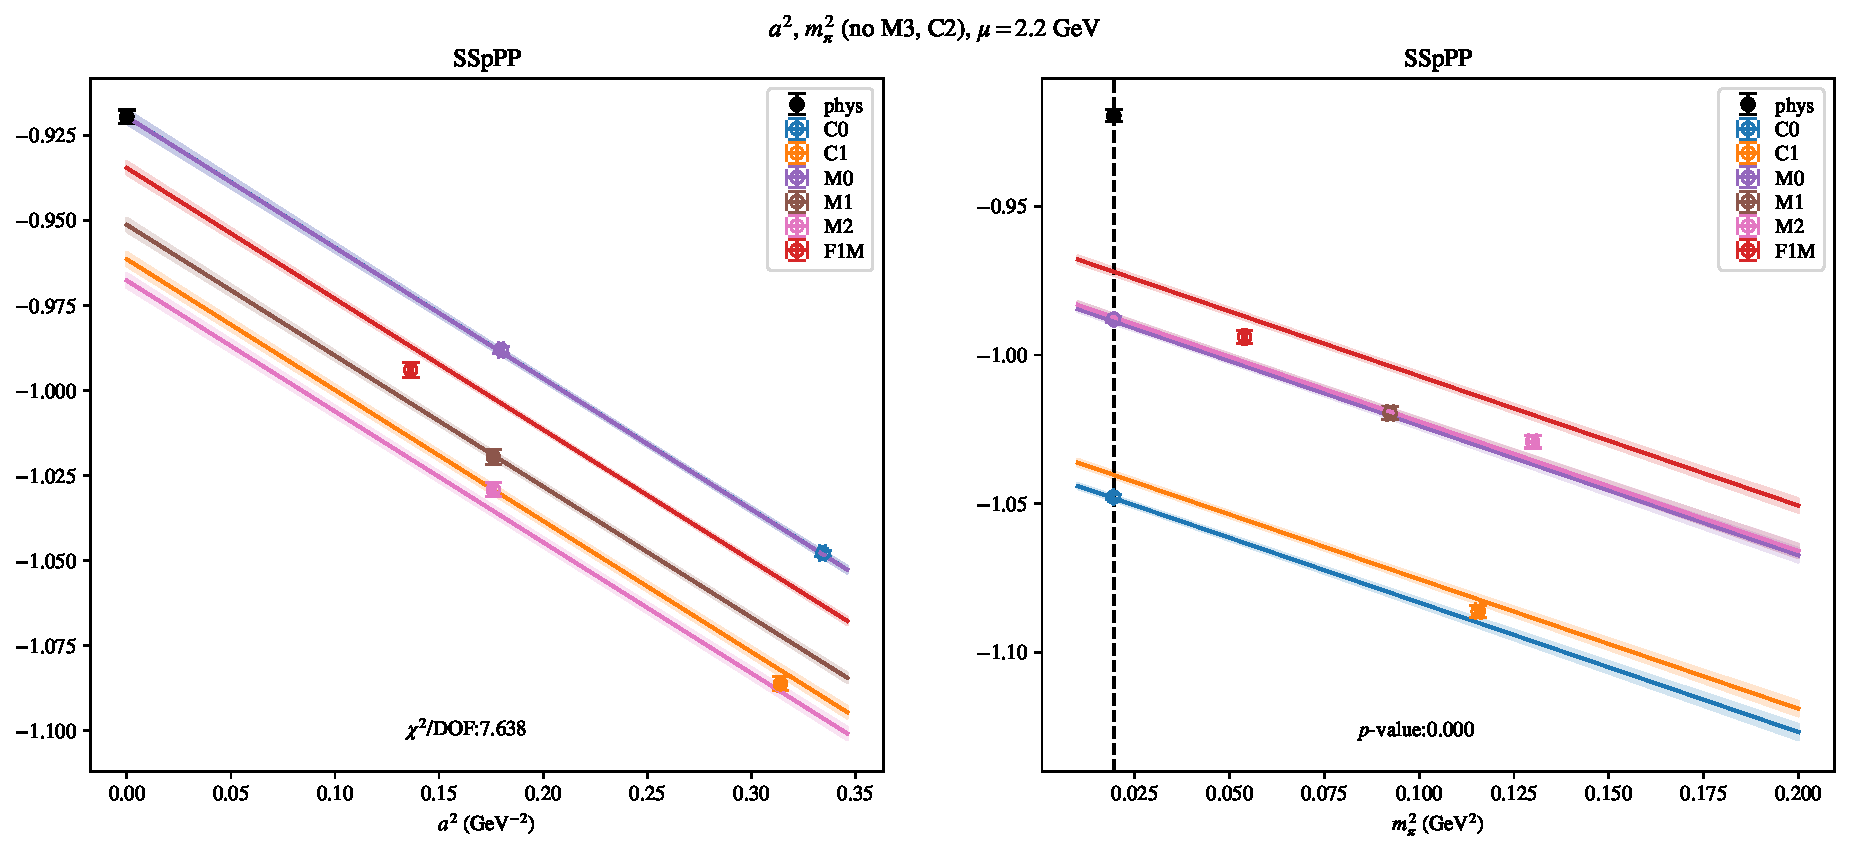
\includepdf[link, pages=-]{VVmAA/SUSY/a2m2mcut_22.pdf}
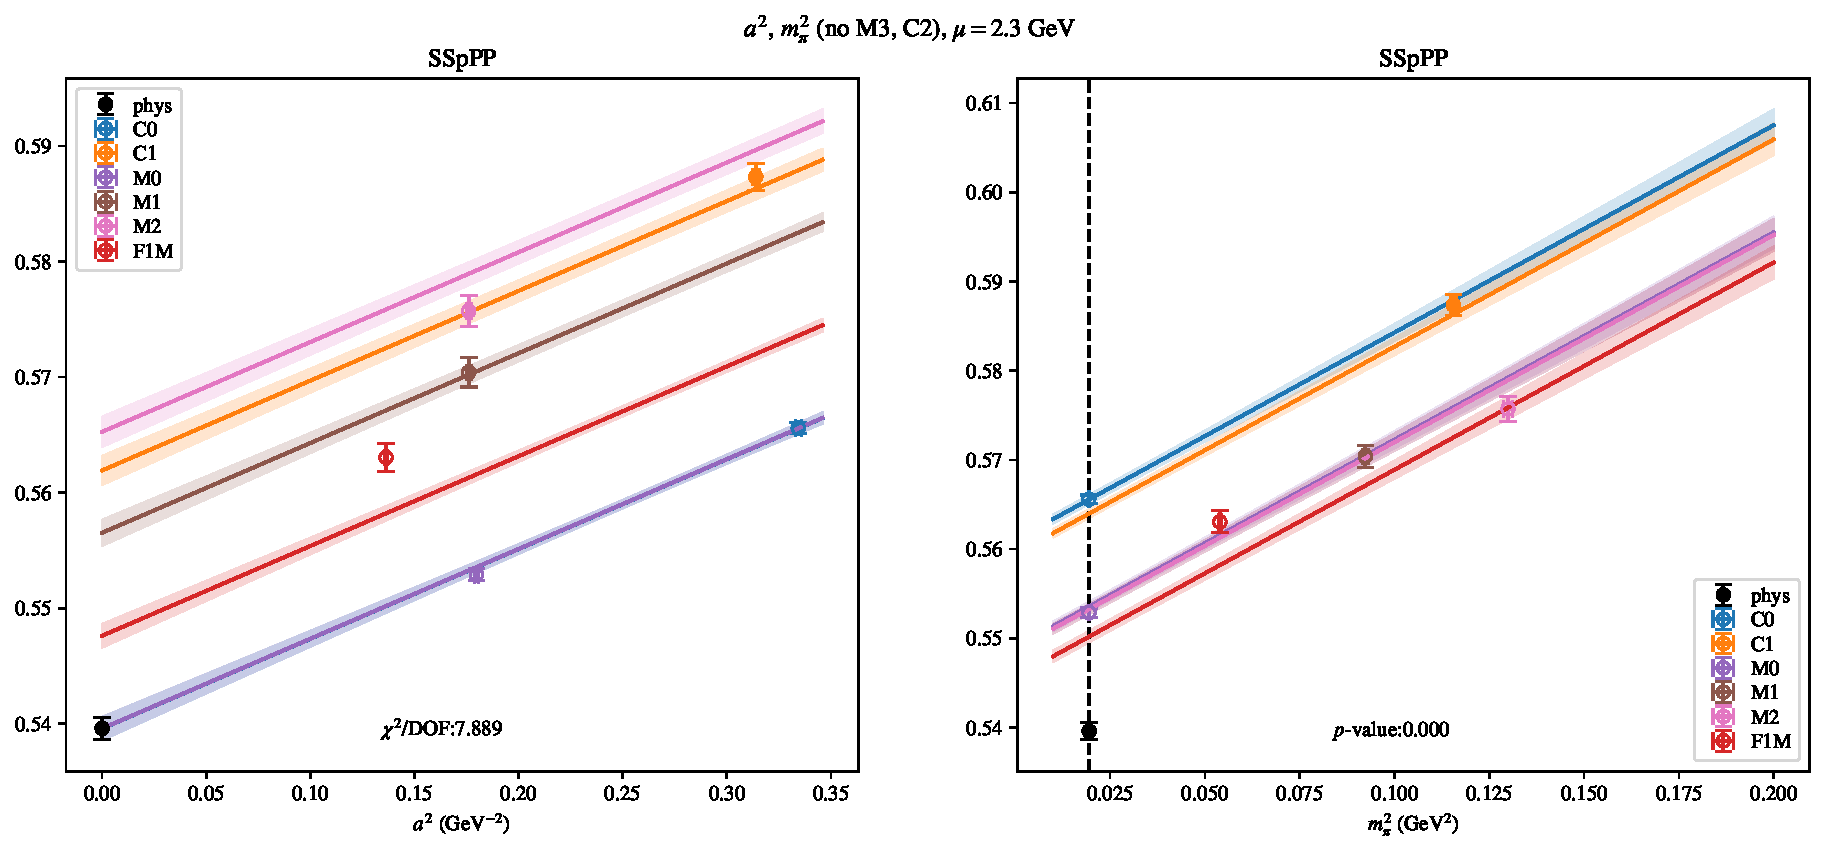
\includepdf[link, pages=-]{VVmAA/SUSY/a2m2mcut_23.pdf}
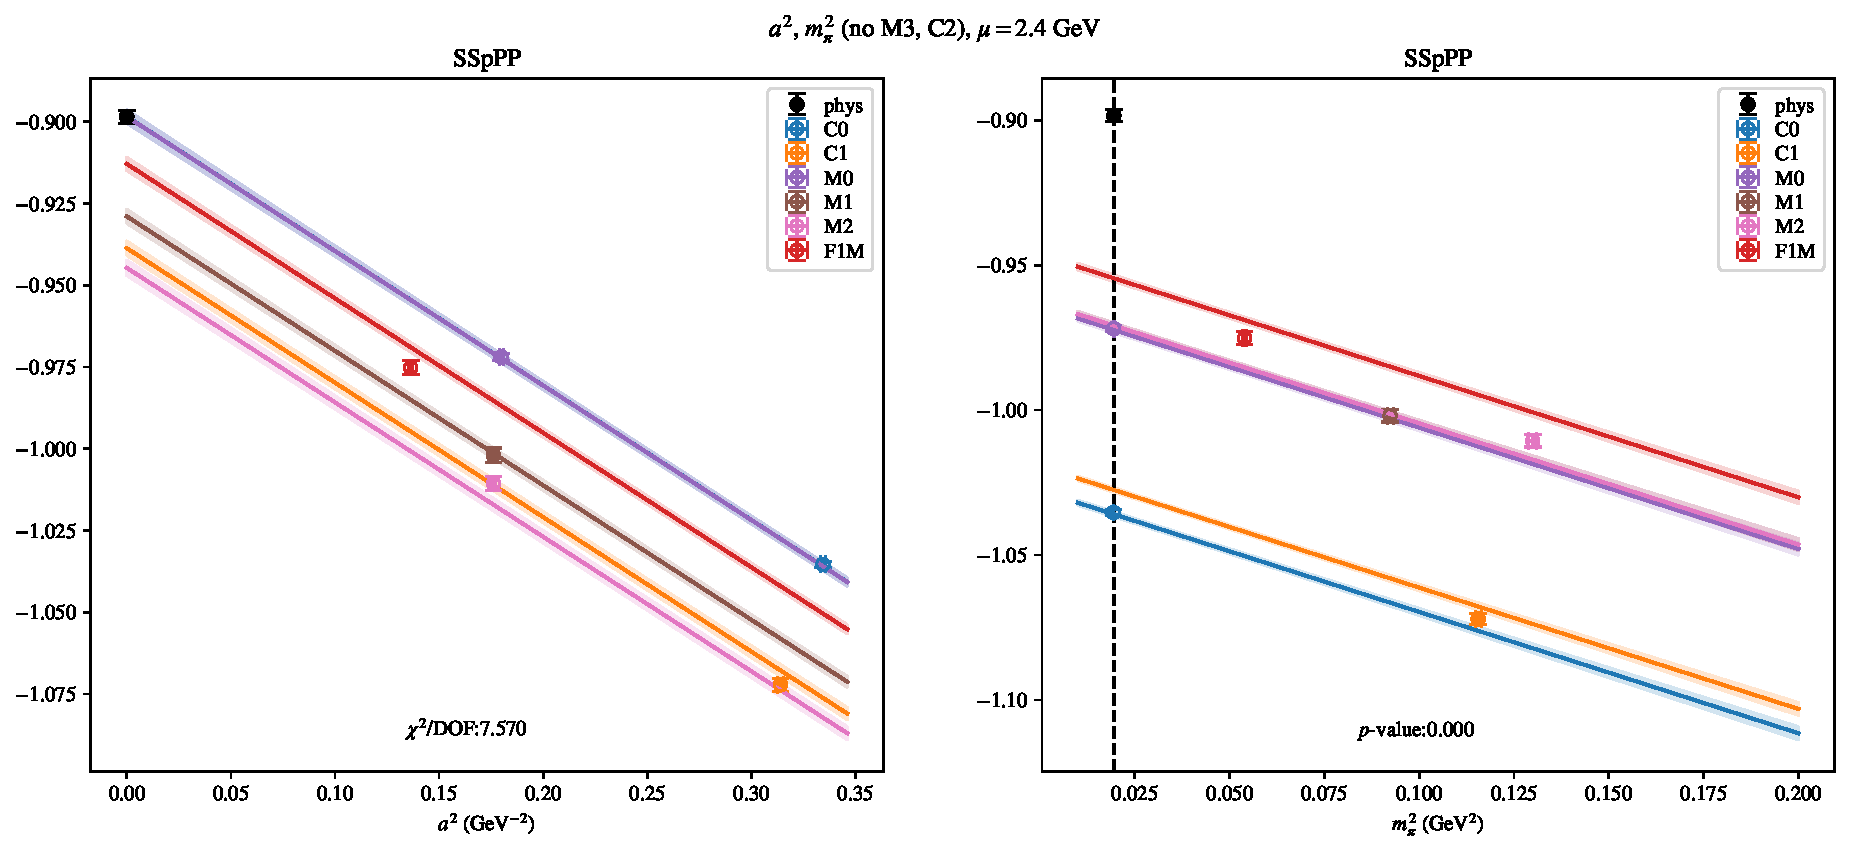
\includepdf[link, pages=-]{VVmAA/SUSY/a2m2mcut_24.pdf}
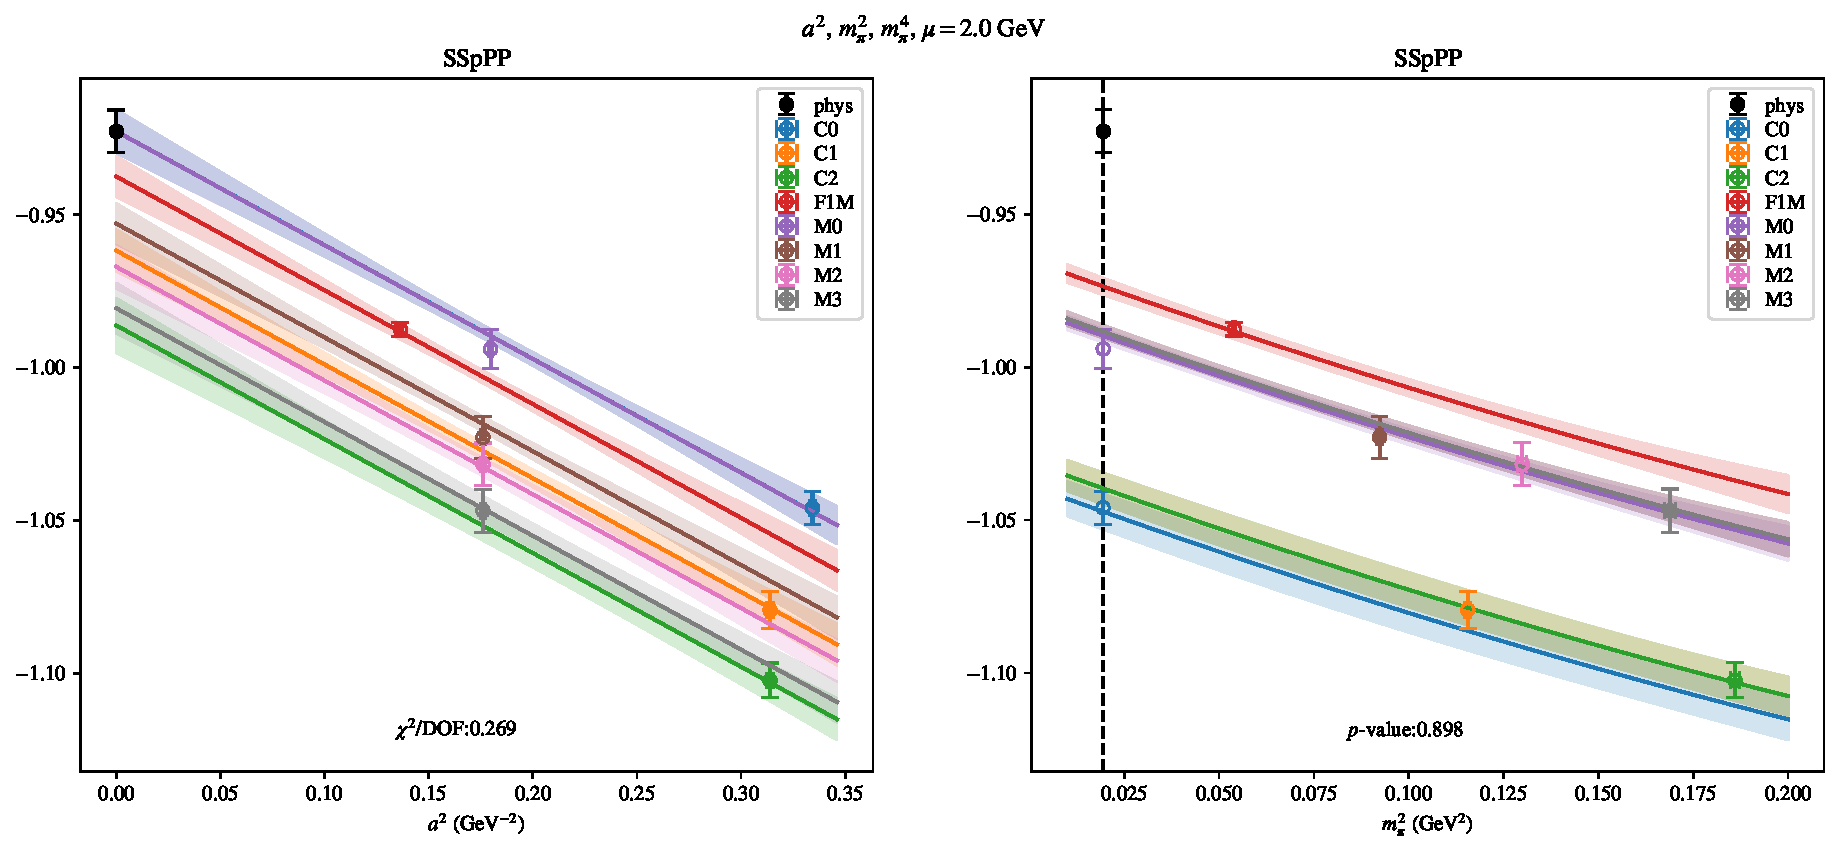
\includepdf[link, pages=-]{VVmAA/SUSY/a2m2m4_20.pdf}
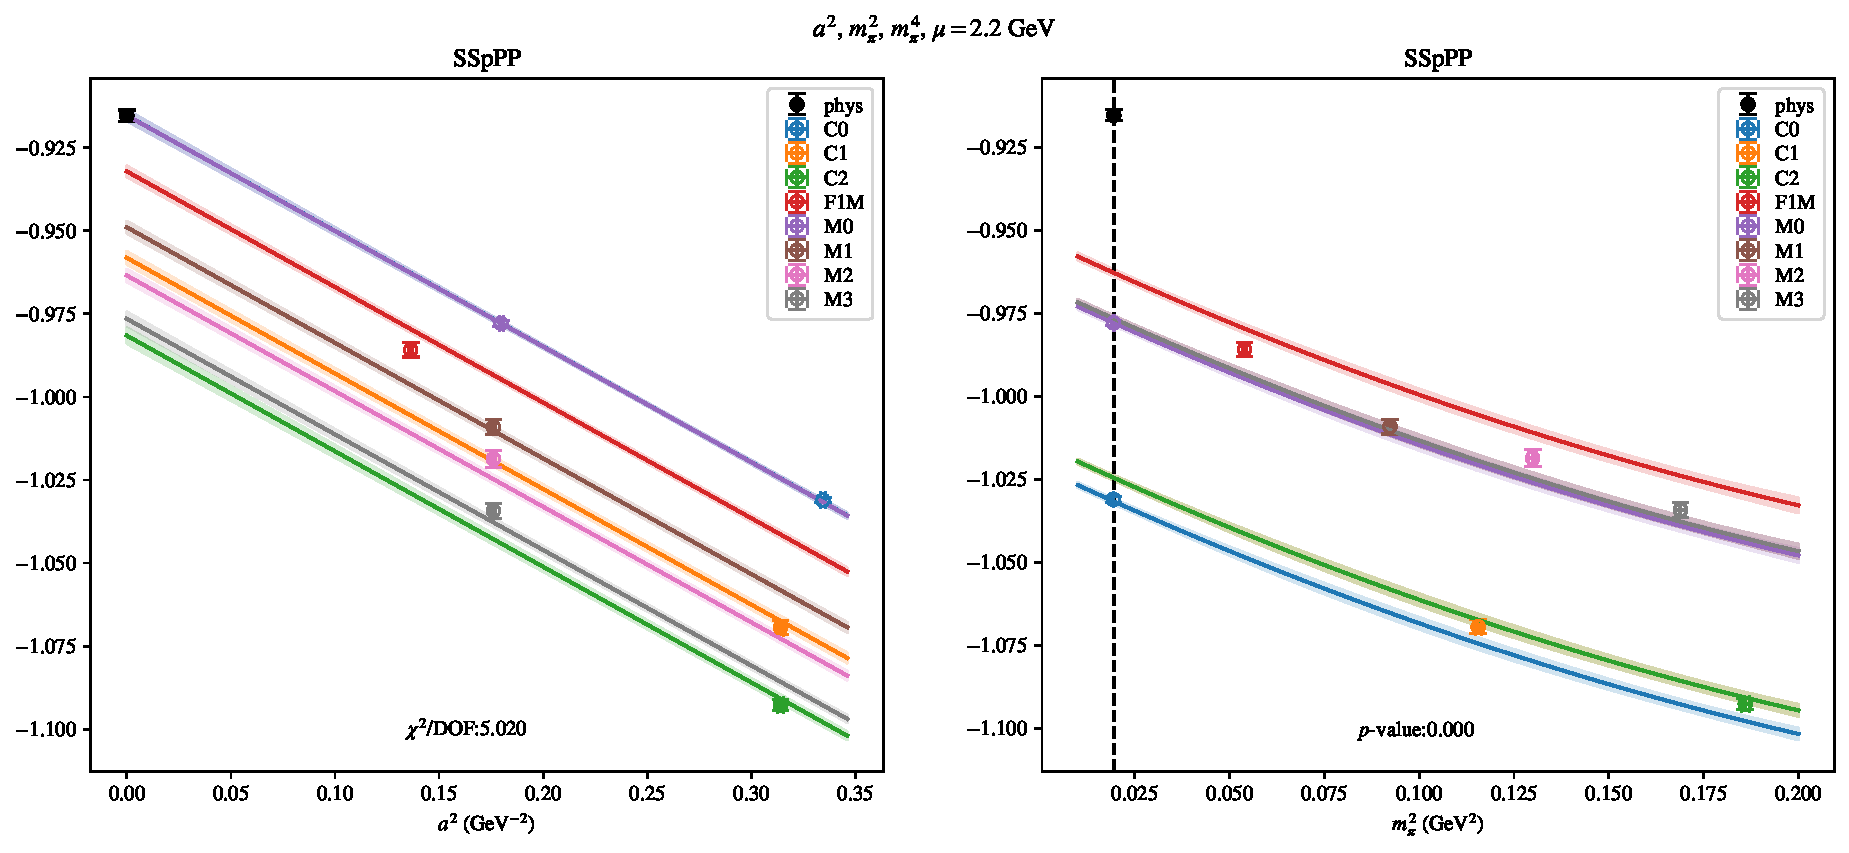
\includepdf[link, pages=-]{VVmAA/SUSY/a2m2m4_22.pdf}
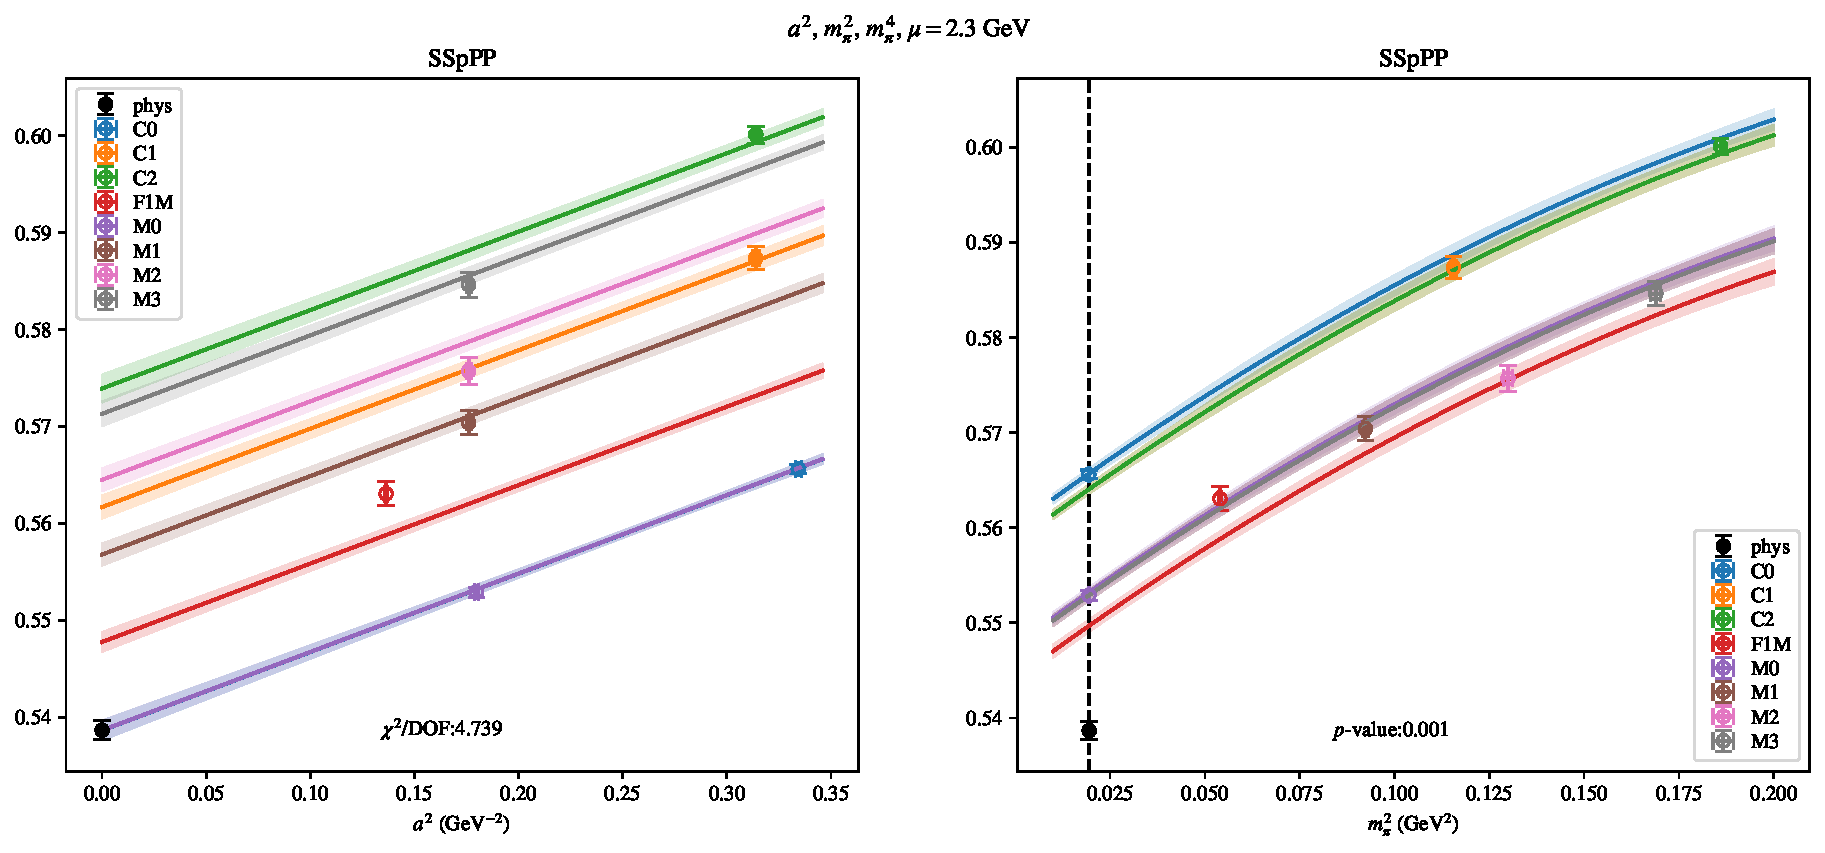
\includepdf[link, pages=-]{VVmAA/SUSY/a2m2m4_23.pdf}
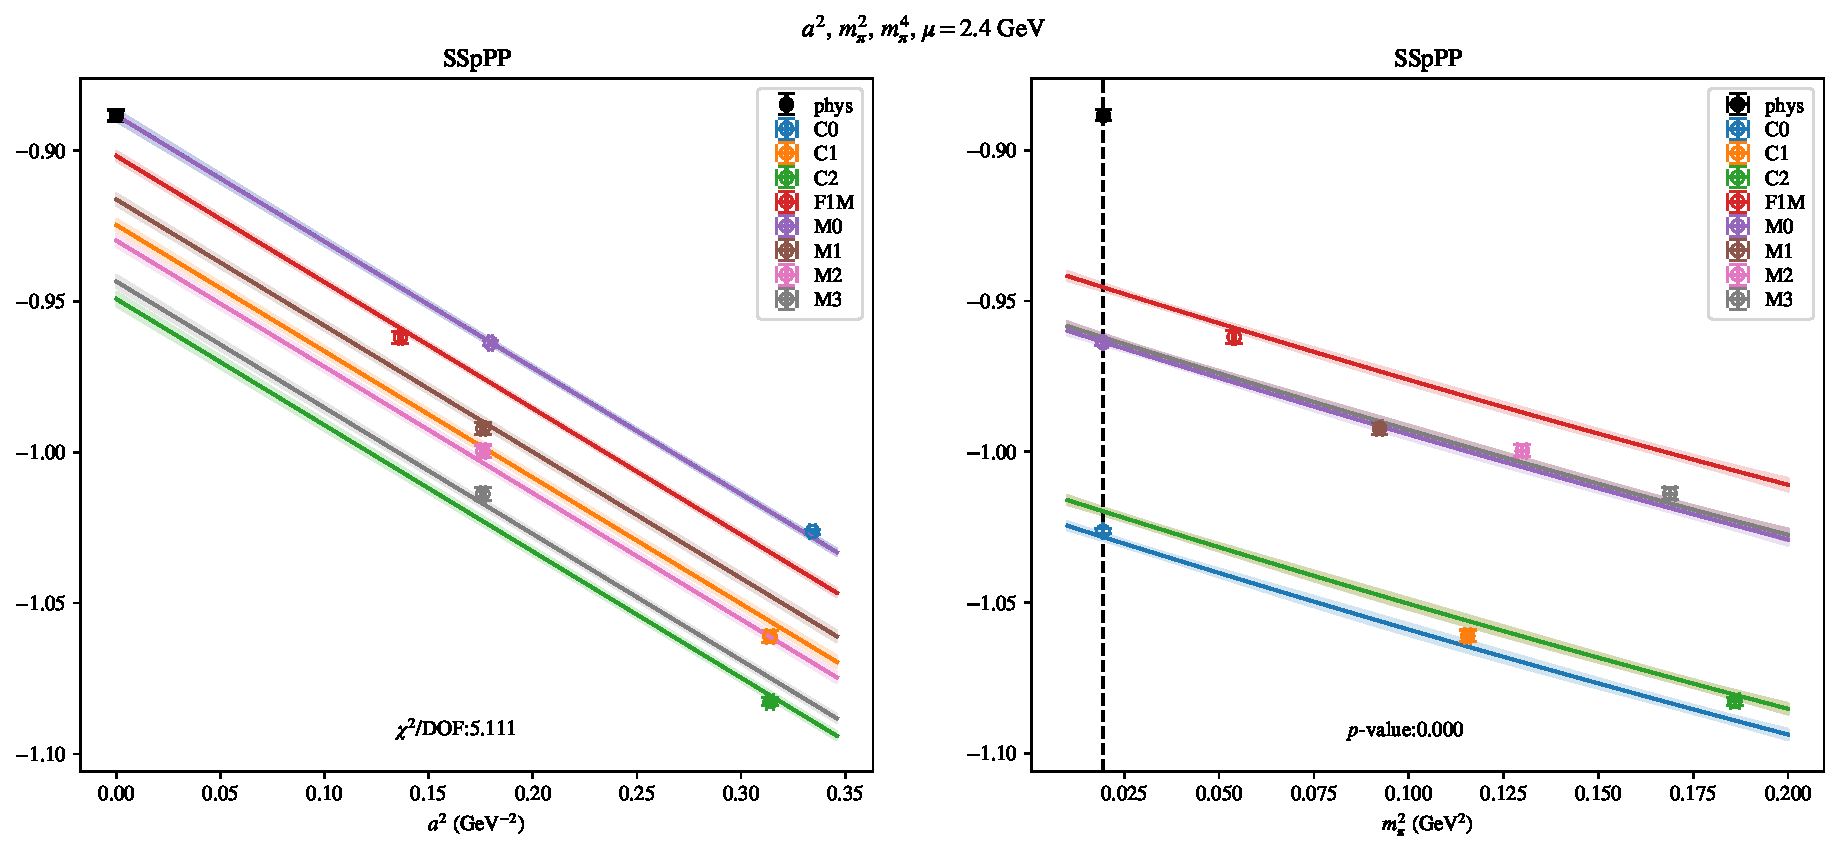
\includepdf[link, pages=-]{VVmAA/SUSY/a2m2m4_24.pdf}
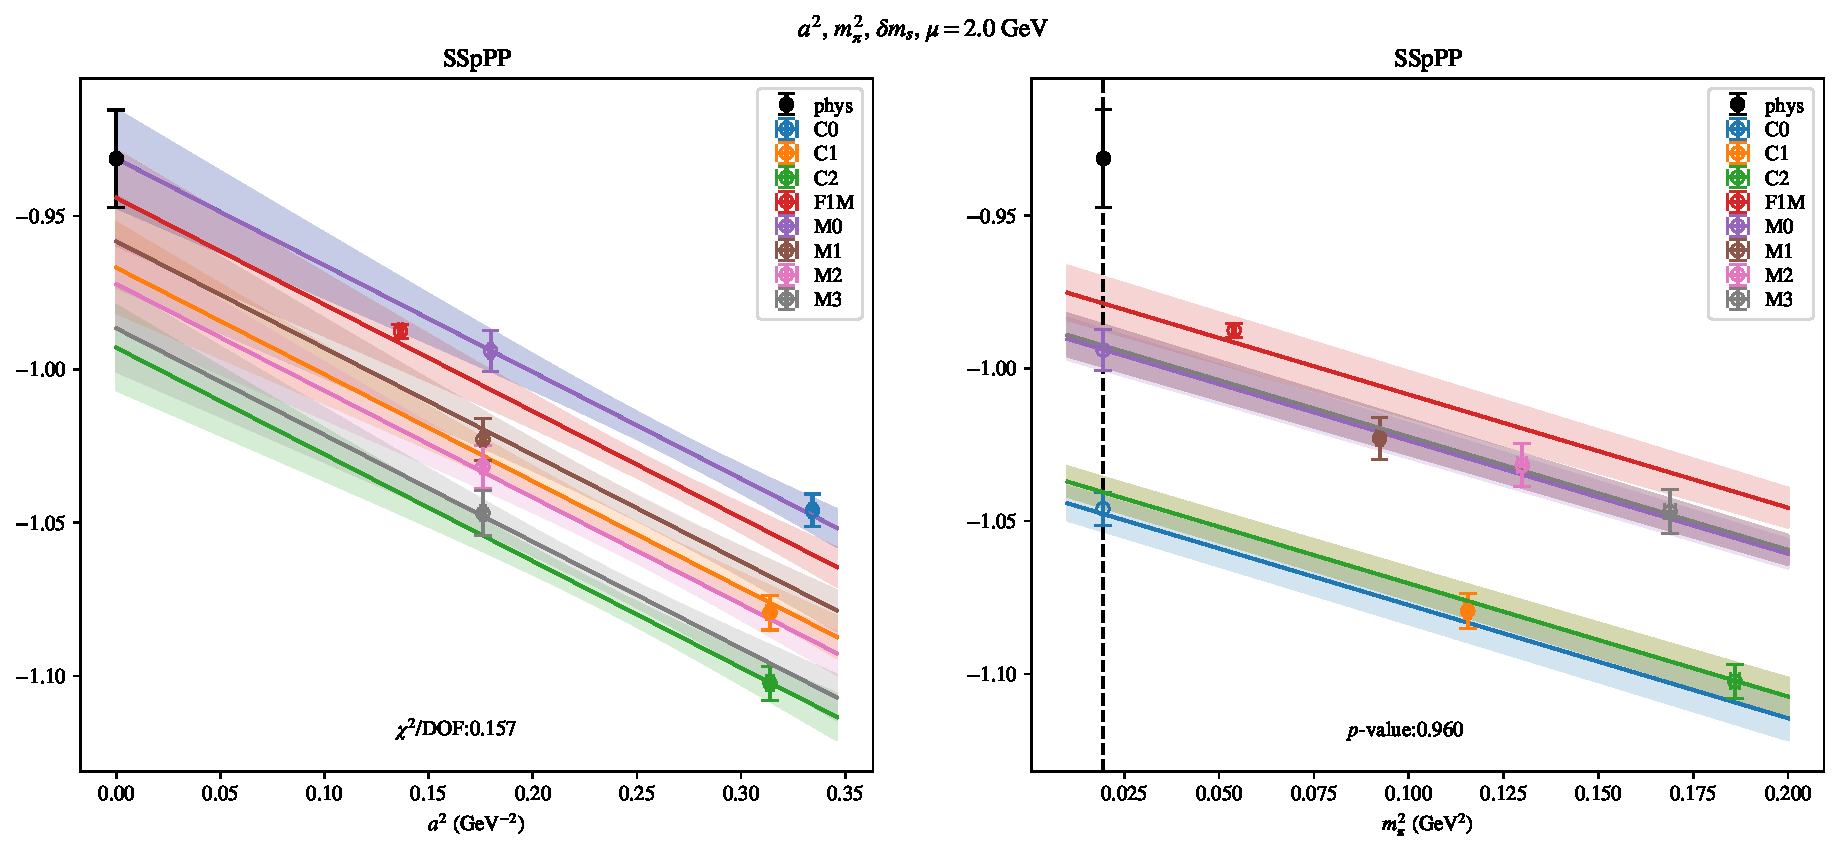
\includepdf[link, pages=-]{VVmAA/SUSY/a2m2delm_20.pdf}
\includepdf[link, pages=-]{VVmAA/SUSY/a2m2delm_22.pdf}
\includepdf[link, pages=-]{VVmAA/SUSY/a2m2delm_23.pdf}
\includepdf[link, pages=-]{VVmAA/SUSY/a2m2delm_24.pdf}
\clearpage
\section{$\mathcal{B}_3$}
\begin{table}[h!]
\begin{center}
\begin{tabular}{|c|c|c|c|c|c|c|}
\hline
$\mu$ (GeV) & $a^2$, $m_\pi^2$& $a^2$, $m_\pi^2$ (no C)& $a^2$, $a^4$, $m_\pi^2$& $a^2$, $m_\pi^2$ (no M3, C2)& $a^2$, $m_\pi^2$, $m_\pi^4$& $a^2$, $m_\pi^2$, $\delta m_s$\\
\hline
2.0& \hyperlink{SSmPP/SUSY/a2m2_20.pdf.1}{\textbf{0.2813(75)}: 0.033 (0.999)} & \hyperlink{SSmPP/SUSY/a2m2noC_20.pdf.1}{\textbf{0.2749(55)}: 0.372 (0.69)} & \hyperlink{SSmPP/SUSY/a2a4m2_20.pdf.1}{\textbf{0.266(78)}: 0.008 (1.0)} & \hyperlink{SSmPP/SUSY/a2m2mcut_20.pdf.1}{\textbf{0.2807(86)}: 0.035 (0.991)} & \hyperlink{SSmPP/SUSY/a2m2m4_20.pdf.1}{\textbf{0.2805(91)}: 0.035 (0.998)} & \hyperlink{SSmPP/SUSY/a2m2delm_20.pdf.1}{\textbf{0.285(30)}: 0.011 (1.0)}\\
2.2& \hyperlink{SSmPP/SUSY/a2m2_22.pdf.1}{\textbf{0.2742(78)}: 0.023 (1.0)} & \hyperlink{SSmPP/SUSY/a2m2noC_22.pdf.1}{\textbf{0.2725(44)}: 0.653 (0.52)} & \hyperlink{SSmPP/SUSY/a2a4m2_22.pdf.1}{\textbf{0.270(48)}: 0.029 (0.998)} & \hyperlink{SSmPP/SUSY/a2m2mcut_22.pdf.1}{\textbf{0.2740(68)}: 0.033 (0.992)} & \hyperlink{SSmPP/SUSY/a2m2m4_22.pdf.1}{\textbf{0.2732(77)}: 0.025 (0.999)} & \hyperlink{SSmPP/SUSY/a2m2delm_22.pdf.1}{\textbf{0.275(21)}: 0.025 (0.999)}\\
2.3& \hyperlink{SSmPP/SUSY/a2m2_23.pdf.1}{\textbf{0.2708(65)}: 0.029 (1.0)} & \hyperlink{SSmPP/SUSY/a2m2noC_23.pdf.1}{\textbf{0.2704(39)}: 0.848 (0.428)} & \hyperlink{SSmPP/SUSY/a2a4m2_23.pdf.1}{\textbf{0.269(47)}: 0.036 (0.997)} & \hyperlink{SSmPP/SUSY/a2m2mcut_23.pdf.1}{\textbf{0.2708(75)}: 0.036 (0.991)} & \hyperlink{SSmPP/SUSY/a2m2m4_23.pdf.1}{\textbf{0.2697(84)}: 0.023 (0.999)} & \hyperlink{SSmPP/SUSY/a2m2delm_23.pdf.1}{\textbf{0.270(17)}: 0.034 (0.998)}\\
2.4& \hyperlink{SSmPP/SUSY/a2m2_24.pdf.1}{\textbf{0.2677(66)}: 0.036 (0.999)} & \hyperlink{SSmPP/SUSY/a2m2noC_24.pdf.1}{\textbf{0.2680(36)}: 1.073 (0.342)} & \hyperlink{SSmPP/SUSY/a2a4m2_24.pdf.1}{\textbf{0.268(40)}: 0.042 (0.997)} & \hyperlink{SSmPP/SUSY/a2m2mcut_24.pdf.1}{\textbf{0.2677(66)}: 0.046 (0.987)} & \hyperlink{SSmPP/SUSY/a2m2m4_24.pdf.1}{\textbf{0.2665(76)}: 0.034 (0.998)} & \hyperlink{SSmPP/SUSY/a2m2delm_24.pdf.1}{\textbf{0.267(16)}: 0.046 (0.996)}\\
\hline
\end{tabular}
\caption{Physical point value from chiral and continuum extrapolation at renormalisation scale $\mu$. Entries are \textbf{value(error)}: $\chi^2/\text{DOF}$ ($p$-value).}
\end{center}
\end{table}
\begin{table}[h!]
\begin{center}
\begin{tabular}{|c c|c|c|c|c|c|c|}
\hline
$\mu$ (GeV) &  & $a^2$, $m_\pi^2$& $a^2$, $m_\pi^2$ (no C)& $a^2$, $a^4$, $m_\pi^2$& $a^2$, $m_\pi^2$ (no M3, C2)& $a^2$, $m_\pi^2$, $m_\pi^4$& $a^2$, $m_\pi^2$, $\delta m_s$\\
\hline
\multirow{2}{0.5in}{2.0} & $\alpha$ & 0.66(21)& 0.85(15)& 1.2(60)& 0.66(23)& 0.67(24)& 0.60(52)\\
 & $\beta$ & 0.0076(28)& 0.00683(34)& 0.0072(22)& 0.0082(38)& 0.0089(26)& 0.0068(23)\\
\hline
\multirow{2}{0.5in}{2.2} & $\alpha$ & 0.75(22)& 0.80(12)& 0.914& 0.74(19)& 0.76(22)& 0.73(39)\\
 & $\beta$ & 0.0072(24)& 0.00680(30)& 0.0071(12)& 0.0077(28)& 0.0090(26)& 0.0071(15)\\
\hline
\multirow{2}{0.5in}{2.3} & $\alpha$ & 0.79(19)& 0.82(10)& 0.838& 0.79(21)& 0.81(24)& 0.80(34)\\
 & $\beta$ & 0.0072(22)& 0.00685(29)& 0.0072(12)& 0.0075(26)& 0.0092(30)& 0.0071(11)\\
\hline
\multirow{2}{0.5in}{2.4} & $\alpha$ & 0.84(20)& 0.845(98)& 0.83& 0.84(19)& 0.86(22)& 0.85(32)\\
 & $\beta$ & 0.0072(21)& 0.00691(29)& 0.0071(11)& 0.0075(23)& 0.0093(26)& 0.0073(11)\\
\hline
\end{tabular}
\caption{Fit values of coefficients in $Q = Q_{phys} + \mathbf{\alpha} a^2 + \mathbf{\beta}\left(\frac{m_\pi^2}{f_\pi^2}-\frac{m_{\pi,PDG}^2}{f_\pi^2}\right) + \ldots$.}
\end{center}
\end{table}
\includepdf[link, pages=-]{SSmPP/SUSY/a2m2_20.pdf}
\includepdf[link, pages=-]{SSmPP/SUSY/a2m2_22.pdf}
\includepdf[link, pages=-]{SSmPP/SUSY/a2m2_23.pdf}
\includepdf[link, pages=-]{SSmPP/SUSY/a2m2_24.pdf}
\includepdf[link, pages=-]{SSmPP/SUSY/a2m2noC_20.pdf}
\includepdf[link, pages=-]{SSmPP/SUSY/a2m2noC_22.pdf}
\includepdf[link, pages=-]{SSmPP/SUSY/a2m2noC_23.pdf}
\includepdf[link, pages=-]{SSmPP/SUSY/a2m2noC_24.pdf}
\includepdf[link, pages=-]{SSmPP/SUSY/a2a4m2_20.pdf}
\includepdf[link, pages=-]{SSmPP/SUSY/a2a4m2_22.pdf}
\includepdf[link, pages=-]{SSmPP/SUSY/a2a4m2_23.pdf}
\includepdf[link, pages=-]{SSmPP/SUSY/a2a4m2_24.pdf}
\includepdf[link, pages=-]{SSmPP/SUSY/a2m2mcut_20.pdf}
\includepdf[link, pages=-]{SSmPP/SUSY/a2m2mcut_22.pdf}
\includepdf[link, pages=-]{SSmPP/SUSY/a2m2mcut_23.pdf}
\includepdf[link, pages=-]{SSmPP/SUSY/a2m2mcut_24.pdf}
\includepdf[link, pages=-]{SSmPP/SUSY/a2m2m4_20.pdf}
\includepdf[link, pages=-]{SSmPP/SUSY/a2m2m4_22.pdf}
\includepdf[link, pages=-]{SSmPP/SUSY/a2m2m4_23.pdf}
\includepdf[link, pages=-]{SSmPP/SUSY/a2m2m4_24.pdf}
\includepdf[link, pages=-]{SSmPP/SUSY/a2m2delm_20.pdf}
\includepdf[link, pages=-]{SSmPP/SUSY/a2m2delm_22.pdf}
\includepdf[link, pages=-]{SSmPP/SUSY/a2m2delm_23.pdf}
\includepdf[link, pages=-]{SSmPP/SUSY/a2m2delm_24.pdf}
\clearpage
\section{$\mathcal{B}_4$}
\begin{table}[h!]
\begin{center}
\begin{tabular}{|c|c|c|c|c|c|c|}
\hline
$\mu$ (GeV) & $a^2$, $m_\pi^2$& $a^2$, $m_\pi^2$ (no C)& $a^2$, $a^4$, $m_\pi^2$& $a^2$, $m_\pi^2$ (no M3, C2)& $a^2$, $m_\pi^2$, $m_\pi^4$& $a^2$, $m_\pi^2$, $\delta m_s$\\
\hline
2.0& \hyperlink{SSpPP/SUSY/a2m2_20.pdf.1}{\textbf{1.7618(79)}: 4.362 (0.001)} & \hyperlink{SSpPP/SUSY/a2m2noC_20.pdf.1}{\textbf{1.661(27)}: 0.374 (0.688)} & \hyperlink{SSpPP/SUSY/a2a4m2_20.pdf.1}{\textbf{1.543(75)}: 0.534 (0.71)} & \hyperlink{SSpPP/SUSY/a2m2mcut_20.pdf.1}{\textbf{1.7577(82)}: 6.871 (0.0)} & \hyperlink{SSpPP/SUSY/a2m2m4_20.pdf.1}{\textbf{1.7701(90)}: 6.084 (0.0)} & \hyperlink{SSpPP/SUSY/a2m2delm_20.pdf.1}{\textbf{1.817(23)}: 0.276 (0.893)}\\
2.2& \hyperlink{SSpPP/SUSY/a2m2_22.pdf.1}{\textbf{1.7855(58)}: 7.529 (0.0)} & \hyperlink{SSpPP/SUSY/a2m2noC_22.pdf.1}{\textbf{1.696(19)}: 0.723 (0.485)} & \hyperlink{SSpPP/SUSY/a2a4m2_22.pdf.1}{\textbf{1.613(40)}: 1.279 (0.276)} & \hyperlink{SSpPP/SUSY/a2m2mcut_22.pdf.1}{\textbf{1.7834(58)}: 11.965 (0.0)} & \hyperlink{SSpPP/SUSY/a2m2m4_22.pdf.1}{\textbf{1.7912(64)}: 8.952 (0.0)} & \hyperlink{SSpPP/SUSY/a2m2delm_22.pdf.1}{\textbf{1.815(10)}: 0.93 (0.445)}\\
2.3& \hyperlink{SSpPP/SUSY/a2m2_23.pdf.1}{\textbf{1.7885(57)}: 8.061 (0.0)} & \hyperlink{SSpPP/SUSY/a2m2noC_23.pdf.1}{\textbf{1.701(18)}: 0.935 (0.392)} & \hyperlink{SSpPP/SUSY/a2a4m2_23.pdf.1}{\textbf{1.621(35)}: 0.951 (0.433)} & \hyperlink{SSpPP/SUSY/a2m2mcut_23.pdf.1}{\textbf{1.7855(53)}: 11.346 (0.0)} & \hyperlink{SSpPP/SUSY/a2m2m4_23.pdf.1}{\textbf{1.7986(62)}: 9.744 (0.0)} & \hyperlink{SSpPP/SUSY/a2m2delm_23.pdf.1}{\textbf{1.815(10)}: 0.984 (0.415)}\\
2.4& \hyperlink{SSpPP/SUSY/a2m2_24.pdf.1}{\textbf{1.7899(59)}: 7.391 (0.0)} & \hyperlink{SSpPP/SUSY/a2m2noC_24.pdf.1}{\textbf{1.704(16)}: 1.185 (0.306)} & \hyperlink{SSpPP/SUSY/a2a4m2_24.pdf.1}{\textbf{1.626(33)}: 1.158 (0.327)} & \hyperlink{SSpPP/SUSY/a2m2mcut_24.pdf.1}{\textbf{1.7905(57)}: 12.773 (0.0)} & \hyperlink{SSpPP/SUSY/a2m2m4_24.pdf.1}{\textbf{1.8012(67)}: 9.634 (0.0)} & \hyperlink{SSpPP/SUSY/a2m2delm_24.pdf.1}{\textbf{1.8185(83)}: 1.192 (0.312)}\\
\hline
\end{tabular}
\caption{Physical point value from chiral and continuum extrapolation at renormalisation scale $\mu$. Entries are \textbf{value(error)}: $\chi^2/\text{DOF}$ ($p$-value).}
\end{center}
\end{table}
\begin{table}[h!]
\begin{center}
\begin{tabular}{|c c|c|c|c|c|c|c|}
\hline
$\mu$ (GeV) &  & $a^2$, $m_\pi^2$& $a^2$, $m_\pi^2$ (no C)& $a^2$, $a^4$, $m_\pi^2$& $a^2$, $m_\pi^2$ (no M3, C2)& $a^2$, $m_\pi^2$, $m_\pi^4$& $a^2$, $m_\pi^2$, $\delta m_s$\\
\hline
\multirow{2}{0.5in}{2.0} & $\alpha$ & 0.135(26)& 0.57(12)& 1.62(59)& 0.150(27)& 0.123(28)& 0.043(47)\\
 & $\beta$ & 0.00047(29)& -0.0002(26)& -0.0009(35)& 0.00058(39)& -0.0016(78)& -0.0007(21)\\
\hline
\multirow{2}{0.5in}{2.2} & $\alpha$ & 0.106(13)& 0.458(84)& 1.16(28)& 0.113(13)& 0.097(14)& 0.056(20)\\
 & $\beta$ & -0.0& -0.0003(23)& -0.0008(22)& -0.0& -0.0017(72)& -0.0006(14)\\
\hline
\multirow{2}{0.5in}{2.3} & $\alpha$ & 0.111(15)& 0.448(75)& 1.12(24)& 0.119(13)& 0.094(15)& 0.064(21)\\
 & $\beta$ & -0.0& -0.0003(23)& -0.0008(17)& -0.0001(23)& -0.0026(67)& -0.0006(13)\\
\hline
\multirow{2}{0.5in}{2.4} & $\alpha$ & 0.113(16)& 0.445(66)& 1.11(22)& 0.117(15)& 0.095(17)& 0.064(18)\\
 & $\beta$ & -0.0& -0.0004(22)& -0.0007(18)& -0.0003(22)& -0.0026(69)& -0.0006(13)\\
\hline
\end{tabular}
\caption{Fit values of coefficients in $Q = Q_{phys} + \mathbf{\alpha} a^2 + \mathbf{\beta}\left(\frac{m_\pi^2}{f_\pi^2}-\frac{m_{\pi,PDG}^2}{f_\pi^2}\right) + \ldots$.}
\end{center}
\end{table}
\includepdf[link, pages=-]{SSpPP/SUSY/a2m2_20.pdf}
\includepdf[link, pages=-]{SSpPP/SUSY/a2m2_22.pdf}
\includepdf[link, pages=-]{SSpPP/SUSY/a2m2_23.pdf}
\includepdf[link, pages=-]{SSpPP/SUSY/a2m2_24.pdf}
\includepdf[link, pages=-]{SSpPP/SUSY/a2m2noC_20.pdf}
\includepdf[link, pages=-]{SSpPP/SUSY/a2m2noC_22.pdf}
\includepdf[link, pages=-]{SSpPP/SUSY/a2m2noC_23.pdf}
\includepdf[link, pages=-]{SSpPP/SUSY/a2m2noC_24.pdf}
\includepdf[link, pages=-]{SSpPP/SUSY/a2a4m2_20.pdf}
\includepdf[link, pages=-]{SSpPP/SUSY/a2a4m2_22.pdf}
\includepdf[link, pages=-]{SSpPP/SUSY/a2a4m2_23.pdf}
\includepdf[link, pages=-]{SSpPP/SUSY/a2a4m2_24.pdf}
\includepdf[link, pages=-]{SSpPP/SUSY/a2m2mcut_20.pdf}
\includepdf[link, pages=-]{SSpPP/SUSY/a2m2mcut_22.pdf}
\includepdf[link, pages=-]{SSpPP/SUSY/a2m2mcut_23.pdf}
\includepdf[link, pages=-]{SSpPP/SUSY/a2m2mcut_24.pdf}
\includepdf[link, pages=-]{SSpPP/SUSY/a2m2m4_20.pdf}
\includepdf[link, pages=-]{SSpPP/SUSY/a2m2m4_22.pdf}
\includepdf[link, pages=-]{SSpPP/SUSY/a2m2m4_23.pdf}
\includepdf[link, pages=-]{SSpPP/SUSY/a2m2m4_24.pdf}
\includepdf[link, pages=-]{SSpPP/SUSY/a2m2delm_20.pdf}
\includepdf[link, pages=-]{SSpPP/SUSY/a2m2delm_22.pdf}
\includepdf[link, pages=-]{SSpPP/SUSY/a2m2delm_23.pdf}
\includepdf[link, pages=-]{SSpPP/SUSY/a2m2delm_24.pdf}
\clearpage
\section{$\mathcal{B}_5$}
\begin{table}[h!]
\begin{center}
\begin{tabular}{|c|c|c|c|c|c|c|}
\hline
$\mu$ (GeV) & $a^2$, $m_\pi^2$& $a^2$, $m_\pi^2$ (no C)& $a^2$, $a^4$, $m_\pi^2$& $a^2$, $m_\pi^2$ (no M3, C2)& $a^2$, $m_\pi^2$, $m_\pi^4$& $a^2$, $m_\pi^2$, $\delta m_s$\\
\hline
2.0& \hyperlink{TT/SUSY/a2m2_20.pdf.1}{\textbf{0.481(15)}: 0.052 (0.998)} & \hyperlink{TT/SUSY/a2m2noC_20.pdf.1}{\textbf{0.4602(80)}: 0.472 (0.624)} & \hyperlink{TT/SUSY/a2a4m2_20.pdf.1}{\textbf{0.43(18)}: 0.011 (1.0)} & \hyperlink{TT/SUSY/a2m2mcut_20.pdf.1}{\textbf{0.481(14)}: 0.059 (0.981)} & \hyperlink{TT/SUSY/a2m2m4_20.pdf.1}{\textbf{0.484(15)}: 0.059 (0.994)} & \hyperlink{TT/SUSY/a2m2delm_20.pdf.1}{\textbf{0.497(58)}: 0.005 (1.0)}\\
2.2& \hyperlink{TT/SUSY/a2m2_22.pdf.1}{\textbf{0.490(11)}: 0.052 (0.998)} & \hyperlink{TT/SUSY/a2m2noC_22.pdf.1}{\textbf{0.4763(64)}: 0.825 (0.438)} & \hyperlink{TT/SUSY/a2a4m2_22.pdf.1}{\textbf{0.45(12)}: 0.014 (1.0)} & \hyperlink{TT/SUSY/a2m2mcut_22.pdf.1}{\textbf{0.490(12)}: 0.052 (0.984)} & \hyperlink{TT/SUSY/a2m2m4_22.pdf.1}{\textbf{0.493(12)}: 0.057 (0.994)} & \hyperlink{TT/SUSY/a2m2delm_22.pdf.1}{\textbf{0.501(40)}: 0.01 (1.0)}\\
2.3& \hyperlink{TT/SUSY/a2m2_23.pdf.1}{\textbf{0.493(12)}: 0.056 (0.998)} & \hyperlink{TT/SUSY/a2m2noC_23.pdf.1}{\textbf{0.4791(57)}: 1.177 (0.308)} & \hyperlink{TT/SUSY/a2a4m2_23.pdf.1}{\textbf{0.46(11)}: 0.016 (1.0)} & \hyperlink{TT/SUSY/a2m2mcut_23.pdf.1}{\textbf{0.493(11)}: 0.061 (0.98)} & \hyperlink{TT/SUSY/a2m2m4_23.pdf.1}{\textbf{0.496(11)}: 0.076 (0.989)} & \hyperlink{TT/SUSY/a2m2delm_23.pdf.1}{\textbf{0.503(38)}: 0.011 (1.0)}\\
2.4& \hyperlink{TT/SUSY/a2m2_24.pdf.1}{\textbf{0.496(12)}: 0.072 (0.996)} & \hyperlink{TT/SUSY/a2m2noC_24.pdf.1}{\textbf{0.4819(53)}: 1.526 (0.217)} & \hyperlink{TT/SUSY/a2a4m2_24.pdf.1}{\textbf{0.46(10)}: 0.019 (0.999)} & \hyperlink{TT/SUSY/a2m2mcut_24.pdf.1}{\textbf{0.495(11)}: 0.082 (0.97)} & \hyperlink{TT/SUSY/a2m2m4_24.pdf.1}{\textbf{0.499(12)}: 0.075 (0.99)} & \hyperlink{TT/SUSY/a2m2delm_24.pdf.1}{\textbf{0.506(34)}: 0.017 (0.999)}\\
\hline
\end{tabular}
\caption{Physical point value from chiral and continuum extrapolation at renormalisation scale $\mu$. Entries are \textbf{value(error)}: $\chi^2/\text{DOF}$ ($p$-value).}
\end{center}
\end{table}
\begin{table}[h!]
\begin{center}
\begin{tabular}{|c c|c|c|c|c|c|c|}
\hline
$\mu$ (GeV) &  & $a^2$, $m_\pi^2$& $a^2$, $m_\pi^2$ (no C)& $a^2$, $a^4$, $m_\pi^2$& $a^2$, $m_\pi^2$ (no M3, C2)& $a^2$, $m_\pi^2$, $m_\pi^4$& $a^2$, $m_\pi^2$, $\delta m_s$\\
\hline
\multirow{2}{0.5in}{2.0} & $\alpha$ & -0.099& 0.24(12)& 1.146& -0.088& -0.1(22)& -0.1(41)\\
 & $\beta$ & 0.0027(31)& 0.00228(25)& 0.0015(88)& 0.0025(39)& 0.0& 0.0013(18)\\
\hline
\multirow{2}{0.5in}{2.2} & $\alpha$ & -0.1(16)& 0.069(90)& 0.614& -0.1(17)& -0.1(18)& -0.2(29)\\
 & $\beta$ & 0.0022(25)& 0.00191(22)& 0.0015(11)& 0.0020(32)& -0.0& 0.0013(11)\\
\hline
\multirow{2}{0.5in}{2.3} & $\alpha$ & -0.1(17)& 0.051(77)& 0.578& -0.1(16)& -0.1(15)& -0.2(29)\\
 & $\beta$ & 0.0022(25)& 0.00180(21)& 0.00144(81)& 0.0019(30)& -0.0& 0.0013(11)\\
\hline
\multirow{2}{0.5in}{2.4} & $\alpha$ & -0.1(17)& 0.028(69)& 0.542& -0.1(16)& -0.2(17)& -0.2(26)\\
 & $\beta$ & 0.0023(24)& 0.00170(21)& 0.00140(81)& 0.0019(28)& -0.001& 0.00125(92)\\
\hline
\end{tabular}
\caption{Fit values of coefficients in $Q = Q_{phys} + \mathbf{\alpha} a^2 + \mathbf{\beta}\left(\frac{m_\pi^2}{f_\pi^2}-\frac{m_{\pi,PDG}^2}{f_\pi^2}\right) + \ldots$.}
\end{center}
\end{table}
\includepdf[link, pages=-]{TT/SUSY/a2m2_20.pdf}
\includepdf[link, pages=-]{TT/SUSY/a2m2_22.pdf}
\includepdf[link, pages=-]{TT/SUSY/a2m2_23.pdf}
\includepdf[link, pages=-]{TT/SUSY/a2m2_24.pdf}
\includepdf[link, pages=-]{TT/SUSY/a2m2noC_20.pdf}
\includepdf[link, pages=-]{TT/SUSY/a2m2noC_22.pdf}
\includepdf[link, pages=-]{TT/SUSY/a2m2noC_23.pdf}
\includepdf[link, pages=-]{TT/SUSY/a2m2noC_24.pdf}
\includepdf[link, pages=-]{TT/SUSY/a2a4m2_20.pdf}
\includepdf[link, pages=-]{TT/SUSY/a2a4m2_22.pdf}
\includepdf[link, pages=-]{TT/SUSY/a2a4m2_23.pdf}
\includepdf[link, pages=-]{TT/SUSY/a2a4m2_24.pdf}
\includepdf[link, pages=-]{TT/SUSY/a2m2mcut_20.pdf}
\includepdf[link, pages=-]{TT/SUSY/a2m2mcut_22.pdf}
\includepdf[link, pages=-]{TT/SUSY/a2m2mcut_23.pdf}
\includepdf[link, pages=-]{TT/SUSY/a2m2mcut_24.pdf}
\includepdf[link, pages=-]{TT/SUSY/a2m2m4_20.pdf}
\includepdf[link, pages=-]{TT/SUSY/a2m2m4_22.pdf}
\includepdf[link, pages=-]{TT/SUSY/a2m2m4_23.pdf}
\includepdf[link, pages=-]{TT/SUSY/a2m2m4_24.pdf}
\includepdf[link, pages=-]{TT/SUSY/a2m2delm_20.pdf}
\includepdf[link, pages=-]{TT/SUSY/a2m2delm_22.pdf}
\includepdf[link, pages=-]{TT/SUSY/a2m2delm_23.pdf}
\includepdf[link, pages=-]{TT/SUSY/a2m2delm_24.pdf}
\clearpage
\end{document}